\documentclass{article}

%\usepackage[nonatbib]{neurips_2020}
\usepackage{fullpage}
\usepackage{subfloat}
\usepackage[T1]{fontenc}    % use 8-bit T1 fonts
\usepackage{nicefrac}       % compact symbols for 1/2, etc.
\usepackage{microtype}      % microtypography
\usepackage{graphicx}
\usepackage[hidelinks]{hyperref}
\usepackage{macro_math}
\usepackage{macro_fan}
\usepackage{stmaryrd}
\usepackage{multirow}
\usepackage[us,12hr]{datetime}
\usepackage[utf8]{inputenc} % allow utf-8 input
\usepackage{caption,subcaption}
%\usepackage{breqn}

% Squished list environment to save space
\newcommand{\squishlist}{
\begin{list}{$\bullet$}
{ \setlength{\itemsep}{0pt}
\setlength{\parsep}{2pt}
\setlength{\topsep}{2pt}
\setlength{\partopsep}{0pt}
\setlength{\itemindent}{2pt}
\setlength{\leftmargin}{0.5cm}
% \setlength{\labelwidth}{1em}
}
}
\newcommand{\squishend}{\end{list}}

%\setlength{\parskip}{0.3em}

\begin{document}

\title{Information Transfer in Multi-Task Learning via a Bias-Variance Decomposition in High Dimensions}
\maketitle
%\date{{\ddmmyyyydate\today} at \currenttime}

\begin{abstract}
	Hard parameter sharing is a widely used approach to learn from multiple tasks in many applications, such as text classification. The idea is that all tasks share the same feature layer, while each task uses a specific output layer for prediction. Intuitively, the performance of hard parameter sharing depends on dataset properties such as their sample sizes. Yet, rigorously formulating such intuition can be technically challenging. This paper analyzes the generalization performance of hard parameter sharing in high-dimensional linear regression, where the sample size and feature dimension become increasingly large in a fixed ratio. We present tight generalization bounds for two canonical cases: (i) multiple tasks with the same feature covariates; (ii) two tasks with arbitrarily different sample sizes and covariance matrices. We also demonstrate that these estimates for the empirical loss of hard parameter sharing are incredibly accurate in modest dimensions. Finally, we explain several intriguing empirical phenomena. For example, increasing one task's sample size helps another task initially by reducing variance, but hurts eventually due to increasing bias. This suggests progressively adding data for optimizing hard parameter sharing, and we validate its efficiency in a text classification task.
%	Multi-task learning is a powerful approach in many applications such as image and text classification. Yet, there is little rigorous understanding of when multi-task learning outperforms single-task learning. In this work, we provide a rigorous study to answer the question in the high-dimensional linear regression setting. We show that a bias-variance tradeoff of multi-task learning determines the effect of information transfer, and develop new concentration bounds to analyze the tradeoff. Our key observation is that three properties of task data, namely \textit{task similarity}, \textit{sample ratio}, and \textit{covariate shift} can affect transfer in the high-dimensional linear regression setting. We relate each property to the bias and variance of multi-task learning and explain three negative effects with decreased task similarity,	increased sample ratio, and covariate shift under increased sample ratio. We validate the three effects on text classification tasks. Inspired by our theory, we show two practical connections of interest.
%	First, single-task results can help to understand when multi-task learning gives gains. Second, incrementally adding training data can mitigate negative transfer and improve multi-task training efficiency.
\end{abstract}

\section{Introduction}\label{sec introduction}

\iffalse
%Multi-task learning is an inductive learning mechanism to improve generalization performance using related task data.
%Many state-of-the-art results in computer vision and natural language processing are obtained using multi-task learning.
Multi-task learning is a powerful approach to improve performance for many tasks in computer vision, natural language processing, and other areas \cite{C97,ZY17,R17}.
%In multi-task learning, having related task data is fundamental to its performance.
%Multi-task learning is particularly powerful when there is limited labeled data for a task to be solved, meanwhile more labeled data from different but related tasks is available.
%By combining multiple information sources, it is possible to share all the information in the same model.
In many settings, multiple source tasks are available to help with predicting a particular target task.
\todo{clarify setting is different from traditional MTL}
%For example, many applications in , and many other areas have been achieved by learning from multiple tasks together.
The performance of multi-task learning depends on the relationship between the source and target tasks \cite{C97}.
%	We define that multi-task learning provides \textit{positive transfer} if it outperforms single-task learning, or \textit{negative transfer} otherwise.
When the sources are relatively different from the target, multi-task learning (MTL) has often been observed to perform worse than single-task learning (STL) \cite{AP16,BS17}, which is referred to as \textit{negative transfer} \cite{PY09}.
While many empirical approaches have been proposed to mitigate negative transfer \cite{ZY17}, a precise understanding of when negative transfer occurs remains elusive in the literature \cite{R17}.
%This phenomenon, known as \textit{negative transfer}, is fundamental to the understanding of multi-task learning.

%Inspired by the theory, we propose an incremental training schedule to improve multi-task training.
%We consider a setting where the target task has limited labeled data and show
%On the other hand, unless the structures across task data are well-understood, applying multi-task learning on several different datasets often result in suboptimal models (or negative transfer in more technical terms).

Understanding negative transfer requires developing generalization bounds that scale tightly with properties of each task data, such as its sample size.
This presents a technical challenge in the multi-task setting because of the difference among task features, even for two tasks.
For Rademacher complexity or VC-based techniques, the generalization error scales down as the sample sizes of all tasks increase, when applied to the multi-task setting \cite{B00,AZ05,M06,MPR16,WZR20}.
Without a tight lower bound for multi-task learning, comparing its performance to single-task learning results in vacuous bounds.
\todo{add more technical motivation (or maybe later)}
From a practical standpoint, developing a better understanding of multi-task learning in terms of properties of task data can provide guidance for downstream applications \cite{RH19}.
%For example, the sample sizes of all tasks are often assumed to be equal \cite{B00,LPTV09,LPVT11}.
%On the other hand, uneven sample sizes (or dominating tasks) have been empirically observed to cause negative transfer \cite{YKGLHF20}.
%The benefit of learning multi-task representations has also been studied for certain half-spaces \cite{} and sparse regression \cite{}.
%When all tasks are sufficiently similar, adding more labeled data improves the generalization performance for predicting a particular task \cite{WZR20}.

%\textbf{Setup and Main Results.}
In this work, we study the bias and variance of multi-task learning in the high-dimensional linear regression setting \cite{HMRT19,BLLT20}.
Our key observation is that three properties of task data, including \textit{task similarity}, \textit{sample ratio}, and \textit{covariate shift}, can affect whether multi-task learning outperforms single-task learning (which we refer to as \textit{positive transfer}).
As an example, we vary each property in Figure \ref{fig_model_shift_phasetrans} for two linear regression tasks and measure the improvement of multi-task learning over single-task learning for a particular task.
We observe that the effect of transfer can be either positive or negative as we vary each property.
These phenomena cannot be explained using previous techniques \cite{WZR20}.
The high-dimensional linear regression setting allows us to measure the three properties precisely.
Here we define each property for the case of two tasks, while our definition applies to general settings.
We refer to the first task as the source task and the second as the target task.
\squishlist
	\item \textbf{Task similarity:} Assume that both tasks follow a linear model with parameters $\beta_1, \beta_2\in\real^p$, respectively.
	We measure the distance between them by $\norm{\beta_1 - \beta_2}$.
	\item \textbf{Sample ratio:} Let $n_1 = \rho_1 \cdot p, n_2 = \rho_2 \cdot p$ be the sample size of each task, where $\rho_1, \rho_2>1$ are both fixed values that do not grow with $p$.
	We measure the source/target sample ratio by $\rho_1 / \rho_2$.
%	Importantly, $\rho_2$ can be a small constant (say $2$) to capture the need for more labeled data.
	\item \textbf{Covariate shift:} Assume that the task features are random vectors with positive semidefinite covariance matrices $\Sigma_1\in\real^{p\times p}$ and $\Sigma_2\in\real^{p\times p}$, respectively.
	%$x = \Sigma_i^{1/2}z$, where $z\in\real^p$ consists of i.i.d. entries with mean zero and unit variance, and is a positive semidefinite matrix.
	We measure covariate shift with matrix $\Sigma_1^{1/2}\Sigma_2^{-1/2}$.
\squishend

%The observations highlight the need to develop generalization bounds that scale tightly with properties of multiple tasks data.
% that only contains limited amount of labeled data.
%Following Hastie et al.  and Bartlett et al. \cite{},

%Let $n_i = \rho_i \cdot p$ denote the data size and $X_i\in\real^{n_i\times p}$ denote the features of task $i$.
%The labels of task $i$ are given by $Y_i = X_i\beta_i + \varepsilon_i$, where $\beta_i\in\real^p$ denotes task $i$'s ground truth parameters and $\varepsilon_i$ denotes i.i.d. random noise with mean zero and variance $\sigma^2$.
We consider a multi-task estimator obtained using a shared linear layer for all tasks and a separate output layer for each task \cite{WZR20}.
This two-layer model is inspired by a commonly used idea of hard parameter sharing in multi-task learning \cite{R17,MTDNN19}.
We consider the bias and variance of the multi-task estimator for predicting a target task and compare its performance to single-task learning.
%This corresponds to minimizing $ \sum_{i=1}^t \norm{X_i B W_i - Y_i}^2$.
%Let $\hat{\beta}_t^{\MTL}$ denote the optimal multi-task estimator for the target task, which is defined precisely in Section \ref{sec_prelim}.
%We revisit the bias-variance tradeoff of $\hat{\beta}_t^{\MTL}$.


\HZ{go to intro}
For a multivariate Gaussian random matrix, this result follows from the classical result for the mean of inverse Wishart distribution \cite{anderson1958introduction}.
For a non-Gaussian random matrix, this result can be obtained using the well-known Stieltjes transform method (cf. Lemma 3.11 of \citet{bai2009spectral}).
\fi


\section{Preliminaries}\label{sec_setup}

We describe the bias-variance tradeoff of our setting more formally.
Recall that we have $t$ labeled tasks available, denoted by $(X_1, Y_1), (X_2, Y_2), \dots, (X_t, Y_t)$, where $X_i\in\real^{n_i\times p}$ and $Y_i\in\real^{n_i}$ for $1\le i\le t$.
%Following \cite{HMRT19,BLLT20}, we assume that for each task $i = 1,2,\dots,t$,  every feature vector is generated as $x = \Sigma_i^{1/2} z$, where $z\in\real^p$ is a random vector with i.i.d. entries of mean zero and unit variance and $\Sigma_i\in\real^{p\times p}$ is a positive semidefinite matrix.
Without loss of generality, let the $t$-th task denote the target task.
For an estimator $\hat{\beta}\in\real^p$, we define the out-of-sample (prediction) loss as
	\begin{align*}
		\te_t(\hat{\beta}) \define \exarg{z}{\exarg{\varepsilon_t}{({(\Sigma_t^{1/2} z)}^{\top}\hat{\beta} - {(\Sigma_t^{1/2})}^{\top}\beta_t)^2}}
		= \exarg{\varepsilon_t}{(\hat{\beta} - \beta_t)^{\top}\Sigma_t(\hat{\beta} - \beta_t)}.
	\end{align*}
The single-task estimator $\hat{\beta}_t^{\STL}$ is given by $(X_t^{\top}X_t)^{-1}X_t^{\top}Y_t$.
The bias-variance trade-off \cite{HTF09} says
	\[ \te_t(\hat{\beta}) =
		\bignorm{\exarg{\varepsilon_t}{\hat{\beta}} - \beta_t}^2 + \exarg{\varepsilon_t}{\bignorm{\hat{\beta} - \exarg{\varepsilon_t}{\hat{\beta}}}^2}. \]
In order to study the trade-off between model-shift bias and variance reduction, we need tight concentration bounds to quantify both effects.
For this purpose, we consider the high-dimensional regime where $n_i$ is a fixed constant $\rho_i > 1$ times $p$ for every $1\le i\le t$, and $p$ is large.
%Recall that $n_i = \rho_i \cdot p$ and we assume $\rho_i > 1$ is a fixed constant for every $1\le i\le t$.

We focus on a setting where $\rho_t$ is a small constant.
This setting captures the need for adding more labeled data to reduce the test error of the target task.
A well-known result for this setting states that $\te_t(\hat{\beta}_t^{\STL}) = \sigma^2 \cdot \tr[(X_t^{\top}X_t)^{-1}\Sigma_t]$ is concentrated around $\frac {\sigma^2} {\rho_t - 1}$ (e.g. Chapter 6 of \cite{S07}), which scales with the data size and noise level of the target task.
However, this result only applies to the single-task setting.
Therefore, our goal is to extend this result to the multi-task setting.

To illustrate our intuition, we begin by considering the setting of two tasks with general covariance matrices.
Recall that $\hat{\beta}_t^{\MTL}$ is defined as $BW_t$ after solving equation \eqref{eq_mtl}.
We decompose the test error of $\hat{\beta}_{t}^{\MTL}$ on the target task into two parts (to be derived in Appendix \ref{app_proof_sec3}) as follows
\begin{align}
	\te_t(\hat{\beta}_t^{\MTL}) =& ~ \hat{v}^2 \bignorm{\Sigma_2^{1/2} (\hat{v}^2 X_1^{\top}X_1 + X_2^{\top}X_2)^{-1}X_1^{\top}X_1 (\beta_1 - \hat{v}\beta_2)}^2 \label{eq_te_model_shift} \\
	&+ \sigma^2\cdot \bigtr{(\hat{v}^2 X_1^{\top}X_1 + X_2^{\top}X_2)^{-1}\Sigma_2}, \label{eq_te_var}
\end{align}
where $\hat{v} = W_2 / W_1$ denotes the ratio of the output layer weights.
%Hence the bias of $\te_t(\hat{\beta}_t^{\STL})$ is zero and its test error is equal to variance, given by $$.

\textbf{Notations.}
When there is no ambiguity, we drop the subscript $t$ from $\te_t(\hat{\beta}_t^{\MTL})$ to $\te(\hat{\beta}_t^{\MTL})$ for simplicity.
We refer to the first task as the source task when there are only two tasks.
We call $M = \Sigma_1^{1/2}\Sigma_2^{-1/2}$ the covariate shift matrix.
%Same for $\hat{\beta}_t^{\STL}$.


\section{A Technical Tool to Quantify the Bias-Variance Trade-off}
\label{sec_main}

We develop a technical tool to derive $\te(\hat{\beta}_t^{\MTL})$ that only depends on the qualities of task data such as data sizes and covariance matrices, for two tasks with general covariances.
Then, we extend the result to more than two tasks that share the same features but have different labels.
Finally, we show a sharp bias-variance tradeoff for transfer learning settings.


\subsection{A Key Lemma using Random Matrix Theory}\label{label_rmt}


\begin{lemma}[Informal statement of Lemma \ref{lem_cov_shift}]\label{lem_cov_shift_informal}
	Suppose $X_1=Z_1\Sigma_1^{1/2}\in \R^{n_1\times p}$ and $X_2=Z_2\Sigma_2^{1/2}\in \R^{n_2\times p}$ with $\rho_1=n_1/p>1$ and $\rho_2=n_2/p>1$.
	Let $M = \Sigma_1^{1/2}\Sigma_2^{-1/2}$ and $\lambda_1, \lambda_2, \dots, \lambda_p$ be the singular values of $M^{\top}M$ in descending order.
	For any constant $\e>0$, w.h.p. over the randomness of $X_1, X_2$, we have that
	\begin{align*}
		\bigtr{(X_1^{\top}X_1 + X_2^{\top}X_2)^{-1}\Sigma_2} = \frac{1}{\rho_1+\rho_2}\cdot \frac1p\bigtr{ (a_1 \Sigma_1 + a_2\Sigma_2)^{-1} \Sigma_2} +\bigo{\|\Sigma_2\| p^{-1/2+\epsilon}},
	\end{align*}
where $(a_1, a_2)$ is the solution to the following deterministic equations:
	\begin{align*}
		a_1 + a_2 = 1- \frac{1}{\rho_1 + \rho_2},\quad a_1 + \frac1{\rho_1 + \rho_2}\cdot \frac{1}{p}\sum_{i=1}^p \frac{\lambda_i^2 a_1}{\lambda_i^2 a_1 + a_2} = \frac{\rho_1}{\rho_1 + \rho_2}.
	\end{align*}
\end{lemma}

\subsection{Applications to Multi-Task and Transfer Learning}

\textbf{Multi-task learning.} applies to the setting of two tasks where their covariance matrices may be arbitrarily different.
The above result also applies to the setting of more than two tasks with the same covariates.
%We extend the above result to any number of tasks that have the same covariates.
%In this section we consider the setting with $k$ many that have the same covariates.
Since the tasks all have the same number of datapoints and covariance matrix, the trade-off between model shift bias and variance will be captured by their task models $\set{\beta_i}_{i=1}^k$.
%For this setting, we derive solutions for the multi-task training and the transfer learning setting that match our insights qualitatively from Section \ref{sec_denoise}.
%Let $B^{\star} = [\beta_1, \beta_2, \dots, \beta_k] \in\real^{p\times k}$ denote the underlying task model parameters.
The formal statement is stated in Theorem \ref{thm_many_tasks} and its proof can be found in Appendix \ref{app_proof_many_tasks}.
%The technical crux of our approach is to derive the asymptotic limit of $\te(\hat{\beta}_t^{\MTL})$ in the high-dimensional setting, when $p$ approaches infinity.
We derive a precise limit of $\bigtr{(X_1^{\top}X_1 + X_2^{\top}X_2)^{-1}\Sigma_2}$, which is a deterministic function that only depends on $\Sigma_1, \Sigma_2$ and $n_1/p, n_2/p$ (see Lemma \ref{lem_cov_shift} in Appendix \ref{app_proof_main} for the result).
Based on the result, we show how to determine positive versus negative transfer as follows.

\begin{theorem}[Informal statement of Theorem \ref{thm_model_shift}]\label{thm_main_informal}
	Let $X_i \in\real^{n_i \times p}$ and $Y_i = X_i\beta_i + \varepsilon_i$, for $i = 1, 2$.
	Suppose that $n_1 = \rho_1 p$ and $n_2 = \rho_2 p$, where $\rho_1>1$ and $\rho_2 >1$ are fixed constants.
	There exists two deterministic functions $\Delta_{\beta}$ and $\Delta_{\vari}$ and a small deterministic error $\delta$ that only depend on $\set{\hat{v}, \Sigma_1^{}, n_1, n_2, \beta_1, \beta_2}$ such that
	\begin{itemize}
		\item If $\Delta_{\vari} - \Delta_{\beta} \ge \delta$, then whp $\te(\hat{\beta}_t^{\MTL}) < \te(\hat{\beta}_t^{\STL})$.
		\item If $\Delta_{\vari} - \Delta_{\beta} \le \delta$, then whp $\te(\hat{\beta}_t^{\MTL}) > \te(\hat{\beta}_t^{\STL})$.
	\end{itemize}
\end{theorem}

Theorem \ref{thm_main_informal} shows nearly tight bounds on the trade-off between model-shift bias and variance reduction.
%determined by the covariate shift matrix and the model shift.
The bounds get tighter and tighter as $\rho_1$ increases.
While the general form of $\Delta_{\vari}$ and $\Delta_{\beta}$ can be quite complex, we will show that they provide nice interpretation for simplified settings later on in Section \ref{sec_insight}.
A formal version of Theorem \ref{thm_main_informal} is presented in Theorem \ref{thm_model_shift} and its proof is presented in Appendix \ref{app_proof_main}.

\textbf{Transfer learning.}
We extend the intuition behind Theorem \ref{thm_main_informal} to transfer learning settings.
We provide an analysis of the transfer function of Taskonomy \cite{ZSSGM18} using our setup.
Specifically, the source task encoder consists of the representations learnt from one or more source tasks.
The transfer function then tries to fit the target task data to the source task encoder.
For more details, we refer the reader to Figure 4 in Taskonomy.

We map the procedure to our setup as follows.
First, we obtain the single-task estimator $\hat{\beta}_i$ from the source tasks, for $1\le i \le t-1$.
This forms the shared representation $B = [\hat{\beta}_1,\hat{\beta}_2,\dots,\hat{\beta}_{t-1}]$.
Then, we learn the output layer $W_t$ on the target task by minimizing the following objective
\begin{align}
	g(W_t) = \bignorm{X_t B W_t - Y_t}^2.
\end{align}
After solving $W_t$, we use $\hat{\beta}_t^{\TL} = B W_t$ as the estimator for the target task.
By comparing $\te(\hat{\beta}_t^{\TL})$ to $\te(\hat{\beta}_t^{\STL})$, we observe a similar trade-off between model-shift bias and variance reduction for this setting.
%We use our tools to compare $\te(B W_t)$ to $\te(\beta_t^{\STL})$.
The formal statement is presented in Theorem \ref{prop_taskonomy} and its proof in Appendix \ref{app_proof_sec4}.



\section{Supplementary Materials for Section \ref{sec_insight}}\label{app_proof_main}

From \cite{WZR20}, we know that we need to explicitly restrict the capacity $r$ of $B$ so that there is transfer between the two tasks.
for the rest of the section, we shall consider the case when $r=1$ we are considering the case of two tasks.
Here, equation \eqref{eq_mtl} simplifies to the following
\begin{align}\label{eq_mtl_2task}
	f(B; w_1, w_2) = \bignorm{X_1 B w_1 - Y_1}^2 + \bignorm{X_2 B w_2 - Y_2}^2,
\end{align}
where $B\in\real^p$ and $w_1, w_2$ are both real numbers.
To solve the above, suppose that $w_1, w_2$ are fixed, by local optimality, we solve $B$ as
\begin{align*}
	& \hat{B}(w_1, w_2) \\
	=& (w_1^2 X_1^{\top}X_1 + w_2^2 X_2^{\top}X_2)^{-1} (w_1 X_1^{\top}Y_1 + w_2 X_2^{\top}Y_2) \\
	=& \frac{1}{w_2} ((\frac{w_1}{w_2})^2 X_1^{\top}X_1 + X_2^{\top}X_2)^{-1} (\frac{w_1}{w_2} X_1^{\top}Y_1 + X_2^{\top}Y_2) \\
	=& \frac{1}{w_2}\bigbrace{\beta_t + ((\frac{w_1}{w_2})^2 X_1^{\top}X_1 + X_2^{\top}X_2)^{-1}\bigbrace{X_1^{\top}X_1(\frac{w_1}{w_2}\beta_s - w^2\beta_t) + (\frac{w_1}{w_2} X_1^{\top}\varepsilon_1 + X_2^{\top}\varepsilon_2)}}.
\end{align*}
As a remark, when $w_1 = w_2 = 1$, we recover the linear regression estimator.
The advantage of using $f(B; w_1, w_2)$ is that if $\theta_1$ is a scaling of $\theta_2$, then this case can be solved optimally using equation \eqref{eq_mtl_2task} \cite{KD12}.

\textbf{Defining the multi-task learning estimator.}
Using a validation set that is sub-sampled from the original training dataset, we get a validation loss as follows
\begin{align}
		\val(\hat{B}; w_1, w_2)
	= & n_1 \cdot \bignorm{\Sigma_1^{1/2}((\frac{w_1}{w_2})^2 X_1^{\top}X_1 + X_2^{\top}X_2)^{-1}X_2^{\top}X_2(\beta_s - \frac{w_1}{w_2}\beta_t)}^2 \nonumber \\
		&+ n_1 \sigma^2 \cdot \bigtr{((\frac{w_1}{w_2})^2 X_1^{\top}X_1 + X_2^{\top}X_2)^{-1}\Sigma_1} \nonumber \\
		&+ n_2 \cdot w^2\bignorm{\Sigma_2^{1/2}((\frac{w_1}{w_2})^2 X_1^{\top}X_1 + X_2^{\top}X_2)^{-1}X_1^{\top}X_1(\beta_s - \frac{w_1}{w_2}\beta_t)}^2 \nonumber \\
		&+ n_2 \cdot \sigma^2 \cdot \bigtr{((\frac{w_1}{w_2})^2 X_1^{\top}X_1 + X_2^{\top}X_2)^{-1}\Sigma_2}. \label{eq_val_mtl}
\end{align}
Let $\hat{w_1}/\hat{w_2}$ be the global minimizer of $\val(\hat{B}; w_1, w_2)$.
We will define the multi-task learning estimator for the target task as
	\[ \hat{\beta}_t^{\MTL} = \hat{w}_{2}\hat{B}(\hat{w}_1, \hat{w}_2). \]

The intuition for deriving $\hat{\beta}_t^{\MTL}$ is akin to performing multi-task training in practice.
Let $\hat{v} = \hat{w_1} / \hat{w_2}$ for the simplicity of notation.
The test loss of using $\hat{\beta}_t^{\MTL}$ for the target task is
\begin{align}
	\te(\hat{\beta}_t^{\MTL}) =&~ \hat{v}^2 \bignorm{\Sigma_2^{1/2}(\hat{v}^2 X_1^{\top}X_1 + X_2^{\top}X_2)^{-1} X_1^{\top}X_1 (\beta_s - \hat{v} \beta_t)}^2 \nonumber \\
			&~ + \sigma^2 \cdot \bigtr{(\hat{v}^2 X_1^{\top}X_1 + X_2^{\top}X_2)^{-1} \Sigma_2}. \label{eq_te_mtl_2task}
\end{align}

Our goal is to study under model and covariate shifts, whether multi-task learning helps learn the target task better than single-task learning.
The baseline where we solve the target task with its own data is
\begin{align*}
	te(\hat{\beta}_t^{\STL}) = \sigma^2 \cdot \bigtr{(X_1^{\top}X_1 + X_2^{\top}X_2)^{-1}}, \text{ where } \hat{\beta}_t^{\STL} = (X_2^{\top}X_2)^{-1} X_2^{\top}Y_2.
\end{align*}
%Clearly, whether $\hat{\beta}_t^{\MTL}$ outperforms $\hat{\beta}_t^{\STL}$ depends on the covariate matrices, the difference of the task models, and the number of per-task data points.

We state several helper lemmas to get a bound on the variance of $\hat{\beta}_t^{\STL}$ and $\hat{\beta}_t^{\MTL}$.
The first lemma, which is a folklore result in random matrix theory, helps determine the asymptotic limit of $\te(\hat{\beta}_t^{\STL})$, as $p$ goes to infinity.

\begin{lemma}\label{lem_minv}[\todo{ref?}]
	Let $X\in\real^{n\times p}$ be a random matrix that contains i.i.d. row vectors with mean $0$ and covariance $\Sigma\in\real^{p\times p}$. Let $A$ be a $p\times p$ matrix that is independent of $X$ and satisfies $\|A\|=\OO(1)$.
	In the setting when $n = c p$ we have that
	\[  \bigtr{(X^{\top}X)^{-1}A} = \frac{1}{c - 1} \frac1p\tr(A\Sigma^{-1}) +\bigo{ p^{-1/2+\epsilon}} \]
for any constant $\e>0$.
\end{lemma}

The second lemma, which deals the inverse of the sum of two random matrices, can be viewed as a special case of Theorem \ref{thm_model_shift}.

\begin{lemma}\label{lem_cov_shift}
	Let $X_i\in\real^{n_i\times p}$ be a random matrix that contains i.i.d. row vectors with mean $0$ and variance $\Sigma_i\in\real^{p\times p}$, for $i = 1, 2$.
	Denote by $M = \Sigma_1^{1/2}\Sigma_2^{-1/2}$ and let $\lambda_1, \lambda_2, \dots, \lambda_p$ be the singular values of $M^{\top}M$ in decreasing order.
	When $n_1 = c_1 p$ and $n_2 = c_2 p$, we have that with high probability over the randomness of $X_1$ and $X_2$, the following equation holds
	\begin{align}%\label{lem_cov_shift_eq}
		\bigtr{(X_1^{\top}X_1 + X_2^{\top}X_2)^{-1}\Sigma_2} = \frac{1}{c_1+c_2}\cdot \bigtr{ \frac{1}{p}\cdot(a_1 M^\top M + a_2)^{-1}} +\bigo{ n^{-1/2+\epsilon}},
	\end{align}
	for any constant $\epsilon>0$, where $a_1, a_2$ are solutions to the following deterministic equations:
	\begin{align}
		a_1 + a_2 = 1- \frac{1}{c_1 + c_2},~ a_1 + \frac{1}{p}\cdot\sum_{i=1}^p \frac{a_1}{(c_1 + c_2)(a_1 + a_2/ \lambda_i^2)} = \frac{c_1}{c_1 + c_2}. \label{eq_a12}
	\end{align}
\end{lemma}
We will give the proof of Lemma \ref{lem_cov_shift} in Section \ref{sec_maintools}.

Finally, we can get a bound tighter than Theorem \ref{thm_model_shift} as follows.
\todo{restate this}
\begin{lemma}\label{prop_model_shift_tight}
		In the setting of Theorem \ref{thm_model_shift}, assume that $\Sigma_1 =\id$,
		$\beta_t$ is i.i.d. with mean $0$ and variance $\kappa^2$ and $\beta_s - \beta_t$ is i.i.d. with mean $0$ and variance $d^2$.
		We set $\Delta_{\beta} = \bigbrace{(1 - \hat{w})^2 \kappa^2 + d^2)} \bigtr{Z}$
		and we have
		\begin{align*}
			\te(\hat{\beta}_t^{\MTL}) \le \te(\hat{\beta}_t^{\STL}) \text{ when: } & \Delta_{\vari} \ge \bigbrace{1 + \sqrt{\frac{p}{n_1}}}^4 \Delta_{\beta}, \\
			\te(\hat{\beta}_t^{\MTL}) \ge \te(\hat{\beta}_t^{\STL}) \text{ when: } & \Delta_{\vari} \le \bigbrace{1 - \sqrt{\frac{p}{n_1}}}^4 \Delta_{\beta}.
		\end{align*}
\end{lemma}



\section{Variance Reduction from Information Transfer}\label{sec_denoise}

In this part, we consider the case of two tasks to show  establish the intuition that adding more data helps in multi-task learning by reducing the variance of the estimator.
We achieve this through tight generalization bounds obtained from random matrix theory.
For the case of two tasks, we identify three factors that determine the type of transfer between tasks: model distance, covariate shift matrix, and data ratio.

Recall that the test error of $\hat{\beta}_{t}^{\MTL}$ consists of two parts
\begin{align}
	\te(\hat{\beta}_t^{\MTL}) = \hat{w}^2 \bignorm{\Sigma_2^{1/2} (\hat{w}^2 X_1^{\top}X_1 + X_2^{\top}X_2)^{-1}X_1^{\top}X_1 (\beta_s - \hat{w}\beta_t)}^2 + \sigma^2\cdot \bigtr{(\hat{w}^2 X_1^{\top}X_1 + X_2^{\top}X_2)^{-1}\Sigma_2}. \label{eq_te_model_shift}
\end{align}
It is not hard to show that the variance of $\hat{\beta}_t^{\MTL}$ is reduced compared to $\hat{\beta}_t^{\STL}$ (following the argument of Proposition \ref{prop_monotone}), i.e.
\[ \sigma^2\cdot \bigtr{(\hat{w}^2 X_1^{\top}X_1 + X_2^{\top}X_2)^{-1}\Sigma_2} \le \sigma^2\cdot \bigtr{(X_2^{\top}X_2)^{-1}\Sigma_2}. \]
Because of model shift however, i.e. $\beta_s \neq \beta_t$.
We can no longer guarantee that $\te(\hat{\beta}_{t}^{\MTL}) \le \te(\hat{\beta}_t^{\STL})$.
The main result of this part show deterministic conditions under which we get positive or negative transfer.
And the conditions depend only on the covariate shift matrix $M$, the difference of the task models, and the number of per-task data points.
In order to characterize $\te(\hat{\beta}_t^{\MTL})$ and $\te(\hat{\beta}_t^{\STL})$, the technical crux of our approach relies on deriving the limit of the trace of matrix inverse in the high-dimensional setting.
To illustrate the idea, we observe that by using Lemma \ref{lem_minv}, we have that
\[ \te(\hat{\beta}_t^{\STL}) = \frac{\sigma^2}{n_2 - p}\bigtr{\Sigma_2^{-1}}. \]
We shall also derive the limit of $\te(\hat{\beta}_t^{\MTL})$.
\todo{write a brief technical overview}

%In this case, $\beta_s$ and $\beta_t$ are different.
%, or implicitly add a regularization on $B$.
%\todo{We focus on the former case in this section.}
%, we consider the case when $r=1$ since there are only two tasks.
%We begin by considering the simplified equation \eqref{eq_mtl_basic} to solve for the target task.
%This is equivalent to setting $W_i = 1$ for the two tasks in equation \eqref{eq_mtl}.
%The result of this simplified setting will set up the ground for solving equation \eqref{eq_mtl} when we also optimize $W_1$ and $W_2$.
%By putting the two tasks together, we get
%\begin{align*}
%	\hat{\beta}_{s,t} &= (X_1^{\top}X_1 + X_2^{\top}X_2)^{-1} (X_1^{\top}Y_1 + X_2^{\top}Y_2) \\
%	&= (X_1^{\top}X_1 + X_2^{\top}X_2)^{-1} \bigbrace{(X_1^{\top}X_1\beta_s + X_2^{\top}X_2\beta_t) + (X_1^{\top}\varepsilon_1 + X_2^{\top}\varepsilon_2)} \\
%	&= \beta_t + (X_1^{\top}X_1 + X_2^{\top}X_2)^{-1}\bigbrace{X_1^{\top}X_1(\beta_s - \beta_t) + (X_1^{\top}\varepsilon_1 + X_2^{\top}\varepsilon_2)}
%\end{align*}
%Hence
%\begin{align}
%	\err(\hat{\beta}_{s,t})
%	&= \bignorm{(X_1^{\top}X_1 + X_2^{\top}X_2)^{-1} X_1^{\top}X_1 (\beta_s - \beta_t)}^2
%	+ \sigma^2 \bigtr{(X_1^{\top}X_1 + X_2^{\top}X_2)^{-1}}, \text{ and} \\
%	\te(\hat{\beta}_{s,t})
%	&= \bignorm{\Sigma_2^{1/2} (X_1^{\top}X_1 + X_2^{\top}X_2)^{-1} X_1^{\top}X_1 (\beta_s - \beta_t)}^2 + \sigma^2\cdot \bigtr{(X_1^{\top}X_1 + X_2^{\top}X_2)^{-1}\Sigma_2} \label{eq_te_model_shift}
%\end{align}

\begin{algorithm}[!t]
	\caption{Comparing the test error of MTL, TL and STL estimators}
	\begin{algorithmic}[1]
		\Input Two regression tasks $(X_1, Y_2)$, $(X_2, Y_2)$.
		\Param Shared body $B$, task-specific prediction heads $W_1, W_2$.
		\State Training the shared body $B$.
		\State Optimizing the task heads on the validation set

		\begin{itemize}
			\item Jointly optimizing both tasks: $\hat{\beta}_t^{\MTL}$
			\item Optimizing the target task: $\hat{\beta}_t^{\TL}$
			\item Single-task training baseline: $\hat{\beta}_t^{\STL}$
		\end{itemize}
		\State Problem statement: Provide conditions to compare the test error of the three estimators on the target task, $\te(\hat{\beta}_t^{\MTL})$, $\te(\hat{\beta}_t^{\STL})$ and $\te(\hat{\beta}_t^{\TL})$.
	\end{algorithmic}
\end{algorithm}

Let ${M} = \hat{w} \Sigma_1^{1/2}\Sigma_2^{-1/2}$ denote the weighted covariate shift matrix. Denote by ${\lambda}_1\ge {\lambda}_2 \ge \dots \ge {\lambda}_p$ the singular values of ${M}^{\top}{M}$. Let $(a_1, a_2)$ be the solutions to the following system of equations
	\be
		 a_1 + a_2 = 1- \frac{p}{n_1 + n_2},~ a_1 + \sum_{i=1}^p \frac{a_1}{(n_1 + n_2)(a_1 + a_2/ \lambda_i^2)} = \frac{n_1}{n_1 + n_2}.\label{eq_a2} \\
		 \ee
		 After obtaining $(a_1,a_2)$, we can solve the following linear equations to get $(a_3,a_4)$:
\begin{gather}
		\left(\frac{n_2}{a_2^2}- \sum_{i=1}^p \frac{1}{ (a_2 + \lambda_i^2a_1)^2  }\right) a_3 -  \left(\sum_{i=1}^p \frac{  \lambda_i^2 }{ (  a_2 + \lambda_i^2a_1)^2  }\right)a_4
		= \sum_{i=1}^p \frac{1 }{ (  a_2 + \lambda_i^2a_1)^2  }, \label{eq_a3} \\
		\left(\frac{n_1}{a_1^2} -  \sum_{i=1}^p \frac{\lambda_i^4   }{  (a_2 + \lambda_i^2a_1)^2  }\right)a_4 -\left(\sum_{i=1}^p \frac{\lambda_i^2  }{  (a_2 + \lambda_i^2a_1)^2  }\right)a_3
		= \sum_{i=1}^p \frac{\lambda_i^2 }{  (a_2 + \lambda_i^2a_1)^2  }. \label{eq_a4}
	\end{gather}
Then we introduce the following matrix
$$Z = \frac{n_1^2}{(n_1 + n_2)^2}\cdot{M} \frac{(1 + a_3)\id + a_4 {M}^{\top}{M}}{(a_2 + a_1 {M}^{\top}{M})^2} {M}^{\top},$$
which can be regarded as the asymptotic limit of $\hat w \Sigma_2^{1/2} (\hat{w}^2 X_1^{\top}X_1 + X_2^{\top}X_2)^{-1}\Sigma_1^{1/2}$. Finally we introduce 
$$\delta:=\left[\frac{n_1 \lambda_1}{(\sqrt{n_1}-\sqrt{p})^2\lambda_p  +  (\sqrt{n_2}-\sqrt{p})^2}\right]^2\cdot \norm{\Sigma_1^{1/2}(\beta_s - \hat{w}\beta_t)}^2.$$
{\cor may be able to get a better bound, but the statement will be long}

We now state our main result for two tasks with both covariate and model shift in the following theorem.

\begin{theorem}\label{thm_model_shift}
	Let $n_1, n_2$ be the number of data points for the source, target task, respectively.
	Let $\hat{w}$ denote the optimal solution for the ratio $w_1/w_2$ in equation \eqref{eq_val_mtl}.
	%Let ${M} = \hat{w} \Sigma_1^{1/2}\Sigma_2^{-1/2}$ denote the weighted covariate shift matrix.
	%Denote by ${\lambda}_1, {\lambda}_2, \dots, {\lambda}_p$ the singular values of ${M}^{\top}{M}$.
	The information transfer is solely determined by two deterministic quantities $\Delta_{\beta}$ and $\Delta_{\vari}$, which show the change of model shift bias and variace, respectively.
	With high probability we have
	\begin{align}
	 	\te(\hat{\beta}_{t}^{\MTL}) \le \te(\hat{\beta}_t^{\STL}) \text{ when: } &\Delta_{\vari} - \Delta_{\beta} \ge \left(\bigbrace{1 + \sqrt{\frac{p} {n_1}}}^4 - 1 \right) \delta \label{upper}\\
		\te(\hat{\beta}_t^{\MTL}) \ge \te(\hat{\beta}_t^{\STL}) \text{ when: } &\Delta_{\vari} - \Delta_{\beta} \le -2\bigbrace{2\sqrt{\frac {p}{n_1}} + \frac{p}{n_1}} \delta, \label{lower}
	\end{align}
	where 
	\begin{align*} %\bigtr{{\Sigma_2^{-1}}}
		\Delta_{\vari} &\define {\sigma^2}\bigbrace{\frac{p}{n_2 - p} -  \frac{1}{n_1 + n_2} \bigtr{(a_1 M^{\top}M + a_2\id)^{-1}} } \\
		\Delta_{\beta} &\define (\beta_s - \hat{w}\beta_t)^{\top} \Sigma_1^{1/2} Z \Sigma_1^{1/2} (\beta_s - \hat{w}\beta_t).
	\end{align*}
%	{\color{blue}To write the bounds in the form \eqref{upper} and \eqref{lower}, we have to define $\wh w$ as the minimizer of
%	$$\frac{\sigma^2}{n_1 + n_2} \bigtr{\frac1{a_1(w) M(w)^{\top}M(w) + a_2(w)\id}}+ \Delta_\beta(w).$$
%	Otherwise, the two bounds has to be written into the form
%	\begin{align*}
%	{\sigma^2}\frac{p}{n_2 - p}\ge \min_w \left\{\frac{\sigma^2}{n_1 + n_2} \bigtr{\frac1{a_1(w) M(w)^{\top}M(w) + a_2(w)\id}} + \Delta_\beta(w)+ \left(\bigbrace{1 + \sqrt{\frac{p} {n_1}}}^4 - 1 \right) \delta(w)\right\},
%	\end{align*}
%	and
%	\begin{align*}
%	{\sigma^2}\frac{p}{n_2 - p}\le \min_w \left\{\frac{\sigma^2}{n_1 + n_2} \bigtr{\frac1{a_1(w) M(w)^{\top}M(w) + a_2(w)\id}}+ \Delta_\beta(w) - 2\bigbrace{2\sqrt{\frac {p}{n_1}} + \frac{p}{n_1}} \delta(w)\right\}.
%	\end{align*}
%	} 
\end{theorem}


%	We have the following conditions that guarantee the type of transfer we can get under model shift.
%	\begin{itemize}

%		\item {\bf Negative transfer:} we have $\te(\hat{\beta}_{s,t}) \ge \te(\hat{\beta}_t)$ when
%			\begin{align}
%				\Delta_{\vari} \le \bigbrace{1 - 4\sqrt{\frac{p}{n_1}} - \frac{2p}{n_1}} {\Delta_{\beta}}
%			\end{align}
%	\end{itemize}
%	\begin{align}
%		{\Delta_{\vari}} \ge \bigbrace{1 + \sqrt{\frac{p}{n_1}}}^2 {\Delta_{\beta}},
%\label{eq_model_shift_pos}
%	\end{align}
%	where
%{\cob
%We have that
%	\begin{align*}
%		&~ {\bignorm{\Sigma_2^{1/2} (X_1^{\top}X_1 + X_2^{\top}X_2)^{-1} X_1^{\top}X_1 (\beta_s - \beta_t)}} \\
%		&\le ~ \Delta_\beta^{1/2}+ \left\|M\frac{(1 + a_3)\id + a_4 M^{\top}M}{(a_1 + a_2 M^{\top}M)} M^{\top}\right\|_{op}^{1/2} \|\Sigma_1^{1/2} (\beta_s - \beta_t)\|_2 \left( 2\sqrt{\frac{p} {n_1}} + \frac{p}{n_1}\right),\\
%		\end{align*}
%		and
%	\begin{align*}
%		&~ {\bignorm{\Sigma_2^{1/2} (X_1^{\top}X_1 + X_2^{\top}X_2)^{-1} X_1^{\top}X_1 (\beta_s - \beta_t)}} \\
%		&\ge ~ \Delta_\beta^{1/2}- \left\|M\frac{(1 + a_3)\id + a_4 M^{\top}M}{(a_1 + a_2 M^{\top}M)} M^{\top}\right\|_{op}^{1/2} \|\Sigma_1^{1/2} (\beta_s - \beta_t)\|_2 \left( 2\sqrt{\frac{p} {n_1}} + \frac{p}{n_1}\right),
%	\end{align*}
%	In the case where the entries of $\beta_s-\beta_t$ are i.i.d. random variables and $\Sigma_1=\id$, we have
%\begin{align*}
%		& \Delta_\beta\left( 1-\sqrt{\frac{p}{n_1}}\right)^4 \le ~ {\bignorm{\Sigma_2^{1/2} (X_1^{\top}X_1 + X_2^{\top}X_2)^{-1} X_1^{\top}X_1 (\beta_s - \beta_t)}}^2 \le ~
%\Delta_\beta\left( 1+\sqrt{\frac{p}{n_1}}\right)^4.
%		\end{align*}
%	}

Theorem \ref{thm_model_shift} shows upper and lower bounds that guarantee positive transfer, which is determined by the change of variance $\Delta_{\vari}$ and a certain model shift bias parameter $\Delta_{\beta}$ determined by the covariate shift matrix and the model shift.
The bounds get tighter and tighter as $n_1 / p$ increases.
%\paragraph{Negative transfer: the Limit caused by model shifts.}
%Next we describe lower bounds that guarantee negative transfer to complement Theorem \ref{thm_model_shift}.
%\begin{theorem}[Negative transfer under model shift]\label{thm_model_shift_neg}
%	In the setting of Theorem \ref{thm_model_shift}, we have $\te(\hat{\beta}_{s,t}) \ge
%\te(\hat{\beta}_t)$ when
%	\begin{align*}
%		\Delta_{\vari} \le \bigbrace{1 - 4\sqrt{\frac{p}{n_1}} - \frac{2p}{n_1}} {\Delta_{\beta}}
%	\end{align*}
%	In the special case that $\beta_s - \beta_t$ is i.i.d. with mean $0$ and variance $d^2$ and $\Sigma_1 = \id$, we can get a tighter lower bound that guarantees negative transfer when
%\begin{align}
%	\Delta_{\vari} \le \bigbrace{1 - \sqrt{\frac{p}{n_1}}}^4 \Delta_{\beta}.\label{eq_model_shift_neg}
%\end{align}
%
%\end{theorem}


%From Lemma \ref{lem_cov_shift}, we know that
%\[ \bigtr{(X_1^{\top}X_1 + X_2^{\top}X_2)^{-1} \Sigma_2} = \frac{1}{n_1 + n_2}\cdot \bigtr{ \bigbrace{a_1\Sigma_2^{-1/2}\Sigma_1\Sigma_2^{-1/2} + a_2\id}^{-1}}, \]
%where $a_1, a_2$ are specified in Theorem \ref{thm_cov_shift}.
%Hence the variance part is reduced by the following amount
%\begin{align}
%	\Delta_{\vari} \define \sigma^2 \cdot \bigbrace{\frac{p}{n_2 - p} - \frac{1}{n_1 + n_2} \bigtr{\bigbrace{a_1 M^{\top}M + a_2\id}^{-1}}}
%\end{align}
%It remains to consider the increment from the first term in $\te(\hat{\beta}_{s,t})$, which is bounded using the following lemma.
%We are now interested in the following quantity


%\todo{For technical reasons, we will consider the test error.}
%\section{Effects of Model Distance, Covariate Shift, and Data Ratio on Information Transfer}\label{sec_insight}
\subsection{Effect of Model Distance on Positive versus Negative Transfer}

As a warm up, we show that when $\beta_s = \beta_t$, then the transfer is always positive.
%Since all tasks share the same underlying model $\beta$, we use a simplified objective as follows.
%\begin{align}
%	\label{eq_mtl_basic}
%	f(w) = \sum_{i=1}^k \norm{X_i w - Y_i}^2.
%\end{align}
%{\bf The distributed learning problem.}
%    \begin{align}
%     f(w) = \sum_{i=1}^k \normFro{X_i w - Y_i}^2. \label{eq_dist}
%   \end{align}
%Equation \eqref{eq_mtl_basic} is simplified from equation \eqref{eq_mtl} by setting $A_i$ to be 1 for all tasks. %can select a model from the subspace of $B$ to fit $(X_i, Y_i)$.

\begin{proposition}\label{prop_monotone}
	Suppose that $n > p$.
  When there is no model shift, i.e. $\beta_s = \beta_t$, adding the source task data always reduces the estimation error and the test error for the target task, i.e.
	\begin{align}
%		\err(\hat{\beta}_{t}^{\MTL})  &\le \err(\hat{\beta}_t^{\STL}), \text{ and} \label{eq_mono_e}\\
		\te(\hat{\beta}_{t}^{\MTL}) &\le \te(\hat{\beta}_t^{\STL}). \label{eq_mono_te}
	\end{align}
\end{proposition}

\begin{proof}
%	Equation \eqref{eq_mono_e} is simply because
%		\[ \err(\hat{\beta}_{s,t}) = \bigtr{(X_1^{\top}X_1 + X_2^{\top}X_2)^{-1}} \le \bigtr{(X_1^{\top}X_1)^{-1}} = \err(\hat{\beta}_t). \]
%	Equation \eqref{eq_mono_te} follows because
	Recall that $\hat{\beta}_t^{\MTL} = \hat{w} \cdot \hat{B}$.
	By the optimality of $\hat{w}$, we have by setting $w = 1$ in equation \eqref{eq_te_mtl}
	\begin{align*}
		\te(\hat{\beta}_t^{\MTL}) &\le \sigma^2 \cdot \bigtr{(X_1^{\top}X_1 + X_2^{\top}X_2)^{-1}\Sigma_2} \\
		&= \sigma^2 \cdot \bigtr{\bigbrace{\Sigma_2^{-1/2}X_1^{\top}X_1\Sigma_2^{-1/2} + \Sigma_2^{-1/2}X_2^{\top}X_2\Sigma^{-1/2}}^{-1}} \\
		&\le \bigtr{\bigbrace{\Sigma_2^{-1/2}X_2^{\top}X_2\Sigma_2^{-1/2}}^{-1}}
			= \bigtr{(X_2^{\top}X_2)^{-1} \Sigma_2} = \te(\hat{\beta}_t^{\STL}),
	\end{align*}
	which concludes the proof.
\end{proof}

As a remark, we can derive a similar result for the estimation error as well. The details are omitted.


We describe examples based on Theorem \ref{thm_model_shift} to show several conceptual insights.

\begin{example}[\textbf{Varying the distance of task models}]
	We consider a simple setting where $\Sigma_1 = \id$.
	Suppose that $\beta_s - \beta_t$ is i.i.d. with mean $0$ and variance $d^2$. Hence the task models have distance $d^2\cdot p$ in expectation.


	We first consider $\Sigma_2 = \id$. In this case, we can simplify $\Delta_{\beta}$ as follows
	\begin{align} \label{eq_delta_simple}
		\Delta_{\beta} \define d^2 \cdot \sum_{i=1}^p \frac{(1 + a_3)\lambda_i^2 + a_4 \lambda_i^4}{(a_1 \lambda_i^2 + a_2)^2}.
	\end{align}
	Now we solve the equations \eqref{eq_a2}, \eqref{eq_a3}, \eqref{eq_a4} to get
	\begin{align}
		a_1 = \frac{c_1(c_1 + c_2 - 1)}{(c_1 + c_2)^2},
		a_2 = \frac{c_2(c_1 + c_2 - 1)}{(c_1 + c_2)^2},
		a_3 = \frac{c_2}{(c_1 + c_2)(c_1 + c_2 - 1)},
		a_4 = \frac{c_1}{(c_1 + c_2)(c_1 + c_2 - 1)}.
	\end{align}
%{\color{blue}if $\Sigma_1=\Sigma_2=\id$, then
%	\begin{align}
%		a_1 = c_1 \left( 1- \gamma_n\right) , \quad
%		a_2 = c_2 \left( 1- \gamma_n\right), \quad
%		a_3 = \frac{\gamma_n c_2}{1-\gamma_n}, \quad
%		a_4 =  \frac{\gamma_n c_1}{1-\gamma_n}.
%	\end{align}
%	where $\gamma_n=p/n$, $c_1=n_1/n$, and $c_2=n_2/n$.
%}

	Then we obtain
	\begin{align}
		\Delta_{\beta} = p \cdot d^2 \cdot \frac{c_1^2 (c_1 + c_2)}{(c_1 + c_2 - 1)^3},
		\Delta_{\vari} = \sigma^2 \cdot \frac{c_1}{(c_2 - 1)(c_1 + c_2 - 1)}.
	\end{align}

	We demonstrate our result with a simulation. (\todo {uses the tighter bound Proposition \ref{prop_model_shift_tight}?})
	We consider a setting where $p = 200$, $n_1 = 90p$, $n_2 = 30p$.
	\todo{Fill in other params.}
	We fix the target task and vary the source task, by varying the task model distance parameter $d$.
	We show that Theorem \ref{thm_model_shift} predicts whether we can get positive or negative transfer.
	Figure \ref{fig_model_shift_phasetrans} shows the result.
	We obtain the following insight from the simulation.
	\begin{itemize}
		\item Adding the source task has the effect of reducing the variance of the estimator, independent of the model shift.
		\item Model shift introduces an additional bias term, which scales with $d^2$, the distance of the two task models.
		Hence, the type of transfer is determined by the tradeoff between the bias caused by model shift and the reduction of variance.
	\end{itemize}
\end{example}



\begin{figure}
	\centering
	\includegraphics[width=0.5\textwidth]{figures/model_shift_phase_transition.eps}
	\caption{Positive vs negative transfer as a parameter of the task model distances.}
	\label{fig_model_shift_phasetrans}
\end{figure}



\subsection{Extension to Many Tasks of the Same Covariates}

In this section we consider the setting with $k$ many that have the same covariates.
Since every task has the same number of data points as well as the same covariance, the only differences between different tasks are their models $\set{\beta_i}_{i=1}^k$.
For this setting, we derive solutions for the multi-task training and the transfer learning setting that match our insights qualitatively from Section \ref{sec_denoise}.

Concretely we will consider the following problem.
\begin{align}
	f(B; W_1, \dots, W_k) = \sum_{i=1}^k \bignorm{X B W_i - Y_i}^2. \label{eq_mtl_same_cov}
\end{align}
By fixing $W_1, W_2, \dots, W_k$, we can derive a closed form solution for $B$ as
\begin{align*}
	\hat{B}(W_1, \dots, W_k) &= (X^{\top}X)^{-1} X^{\top} \bigbrace{\sum_{i=1}^k Y_i W_i^{\top}} (Z Z^{\top})^{-1} \\
	&= \sum_{i=1}^k \bigbrace{\beta_i W_i^{\top}} (ZZ^{\top})^{-1} + (X^{\top}X)^{-1}X^{\top} \bigbrace{\sum_{i=1}^k \varepsilon_i W_i^{\top}} (ZZ^{\top})^{-1}
\end{align*}
where we denote $Z\in\real^{r\times k}$ as the $k$ vectors $W_1, W_2, \dots, W_k$ stacked together.
%Now we switch $\hat{B}$ back into equation \eqref{eq_mtl_same_cov} to
Similar to Section \ref{sec_setup}, we consider minimizing the validation loss over $W_1, W_2, \dots, W_k$ provided with $\hat{B}$.

\paragraph{Jointly minimizing over all tasks.}
Denote by $\varepsilon(W) = \sum_{i=1}^k \varepsilon_i W_i^{\top}$.
We shall decompose the validation loss $\val(\hat{B}; W_1, \dots, W_k)$ into two parts.
The first part is the model shift bias, which is equal to
\begin{align*}
	\sum_{j=1}^k \bigbrace{\bignorm{\Sigma^{1/2}\bigbrace{\sum_{i=1}^k(\beta_i W_i^{\top}) (ZZ^{\top})^{-1} W_j - \beta_j}}^2}
\end{align*}
The second part is the variance, which is equal to
\begin{align*}
	& \sum_{j=1}^k \exarg{\varepsilon_i, \forall i}{\bigbrace{\bigbrace{\sum_{i=1}^k \varepsilon_i W_i^{\top}} (ZZ^{\top})^{-1} W_j}^2} \cdot {\bigtr{\Sigma(X^{\top}X)^{-1}}} \\
	=& \sigma^2 \cdot \bigtr{\Sigma (X^{\top}X)^{-1}}.
\end{align*}
Therefore we shall focus on the minimizer for the model shift bias since the variance part does not depend the weights.
Let us denote $Q\in\real^{k\times k}$ where the $(i,j)$-th entry is equal to $W_i^{\top} (ZZ^{\top})^{-1} W_j$, for any $1\le i, j\le k$.
Let $B^{\star} = [\beta_1, \beta_2, \dots, \beta_k] \in\real^{p \times k}$ denote the true model parameters.
We can now write the validation loss succinctly as follows.
\begin{align*}
	\val(\hat{B}; W_1, \dots, W_k) = \sum_{j=1}^k \bignorm{\Sigma^{1/2} \bigbrace{B^{\star} Q - \beta_j}}^2 + \sigma^2 \cdot \bigtr{\Sigma (X^{\top}X)^{-1}}
\end{align*}
From the above we can solve for $Q$ optimally as \todo{this}.

\paragraph{Minimizing over the target task alone.}
If we only minimize over the the validation loss for the target task, we shall get the following.
\begin{align*}
	\val_j(\hat{B} W_j) = \bignorm{\Sigma^{1/2}\bigbrace{\sum_{i=1}^k W_i^{\top} (ZZ^{\top})^{-1}W_j \beta_i - \beta_j}}^2
	+ \sigma^2 \cdot W_j^{\top} (ZZ^{\top})^{-1} W_j \cdot \bigtr{\Sigma (X^{\top}X)^{-1}}.
\end{align*}

From the above we can obtain three conceptual insights that are consistent with Section \ref{sec_denoise} and \ref{sec_insight}.
\begin{itemize}
	\item The de-noising effect of multi-task learning.
	\item Multi-task training vs single-task training can be either positive or negative.
	\item Transfer learning is better than the other two. And the improvement over multi-task training increases as the model distances become larger.
\end{itemize}





\section{Effect of Covariate Shift and Data Ratio on Transfer Rate}

%\subsubsection{Gains over Single-Task Training}

\paragraph{A precise bound when there is no model shift.}
As Proposition \ref{prop_monotone} shows, if $\beta_s$ and $\beta_t$ are equal, then adding the source task dataset always helps learn the target task.
The goal of this section is to understand how covariate shift affects the rate of transfer. \todo{add conceptual msg}

%The key quantity is to look at:
%The estimator using the source and target together from minimizing \eqref{eq_mtl_basic} is
%\[ \hat{\beta}_{s,t} = (X_1^{\top} X_1 + X_2^{\top} X_2)^{-1} (X_1^{\top}Y_1 + X_2^{\top}Y_2)\]
%The estimation error of $\hat{\beta}_{s,t}$ is
%\begin{align}\label{eq_two_task}
%  \err(\hat{\beta}_{s,t}) = \sigma^2 \cdot \tr[(X_1^{\top}X_1 + X_2^{\top} X_2)^{-1}].
%\end{align}
%The estimation error using the target alone is
%\begin{align}\label{eq_target_task}
%	\err(\hat{\beta}_t) = \sigma^2 \cdot \tr[(X_2^{\top} X_2)^{-1}].
%\end{align}
%The improvement of estimation error from adding the source task is then given by
%$\err(\hat{\beta}_t) - \err(\hat{\beta}_{s,t})$.
%For the test error on the target task, the improvement from adding the source task is
%\[ \te(\hat{\beta}_t) - \te(\hat{\beta}_{s,t}) = \sigma^2\cdot\bigtr{\bigbrace{(X_2^{\top}X_2)^{-1} - (X_1^{\top}X_1 + X_2^{\top}X_2)^{-1}}\cdot\Sigma_2}. \]

%We calculate the amount of improvement by comparing equation \eqref{eq_two_task} to equation \eqref{eq_target_task}.
A simple observation here is that when $\beta_s = \beta_t$, the optimal $\hat{w}$ for minimizing equation \eqref{eq_te_mtl} is equal to $1$.
Based on this observation, we can get a more precise result than Theorem \ref{thm_model_shift} on the improvement of adding the source task data that only depends on the covariance matrices $\Sigma_1, \Sigma_2$ and the number of data points $n_1, n_2$.

\begin{proposition}[Transfer rate without model shift]\label{thm_cov_shift}
	When $\beta_s = \beta_t$, we have that the optimal ratio for $W_1/W_2$ in equation \eqref{eq_te_mtl} satisfies 
	$$1\le \hat{w} \le w_0:=1 +\frac{\sigma^2  \bigtr{(M^\top Z_1^{\top}Z_1 M)^{-1}} }{\left\|( M^\top Z_1^{\top}Z_1 M + Z_2^{\top}Z_2)^{-1} M^\top Z_1^{\top} Z_1 \Sigma_1^{1/2}\beta_t \right\|^2},$$%is $\hat{w} = 1 \pm \bigo{\frac 1 {n_1+n_2}}$ \todo{(figure out the constants)}
	where $M:=\Sigma_1^{1/2}\Sigma_2^{-1/2}$. 
	And
	\begin{align*}
		%\err(\hat{\beta}^{\TL}_{s,t}) &= \sigma^2 \cdot \bigtr{\frac 1 {(n_1 + n_2)a_1\Sigma_1 + (n_1 + n_2)a_2\Sigma_2}} \\
		\te(\hat{\beta}^{\TL}_{t}) &= \sigma^2 \cdot \bigtr{\bigbrace{(n_1 + n_2)a_1\Sigma_2^{-1/2}\Sigma_1\Sigma_2^{-1/2} + (n_1 + n_2)a_2\id}^{-1}} + \bigo{|w_0-1|},
	\end{align*}
where $a_1, a_2$ are the solutions of equations \eqref{eq_a2}. \cor $w_0$ is close to 1 if the signal strength $\beta_t$ is much larger than the noise strength \nc
\end{proposition}

% \begin{proposition}[Transfer rate without model shift] 
%	Suppose $\beta_s = \beta_t$ with i.i.d. entries of mean zero and variance $d^2$. Then we have that the optimal ratio for $W_1/W_2$ in equation \eqref{eq_te_mtl} satisfies 
%	$$1\le \hat{w} \le w_0:=1 + \frac{\sigma^2  \bigtr{(M^\top Z_1^{\top}Z_1 M)^{-1}} }{\left\|( M^\top Z_1^{\top}Z_1 M + Z_2^{\top}Z_2)^{-1} M^\top Z_1^{\top} Z_1 \Sigma_1^{1/2}\beta_t \right\|^2},$$ 
%	where $\|\Sigma_1\|_{\min}$ is the smallest singular value of $\Sigma_1$. Note that $w_0$ is very close to $1$ up to a small error of order $n_1^{-1}$.
%\end{proposition}
\begin{proof}
We abbreviate $\val(w_2\hat{B}(w)):=\val(w)$. We first notice that $\val (w) < \val (1)$ for all $0\le w < 1$. Thus we have $\hat w\ge 1$. It suffices to consider the case with $w> 1$. Under the assumption on $\beta_s$ and $\beta_t$, we can write
\begin{align}
	\val(w) =&~  \left( 1-\frac1w\right)^2 \left\|( M^\top Z_1^{\top}Z_1 M + w^{-2}Z_2^{\top}Z_2)^{-1} M^\top Z_1^{\top} Z_1 \Sigma_1^{1/2}\beta_t \right\|^2 \nonumber \\
			&~ + \frac{\sigma^2}{w^2} \cdot \bigtr{( M^\top Z_1^{\top}Z_1 M + w^{-2}Z_2^{\top}Z_2)^{-1} }. \nonumber
\end{align}
Since 
$$\left\|( M^\top Z_1^{\top}Z_1 M + w^{-2}Z_2^{\top}Z_2)^{-1} M^\top Z_1^{\top} Z_1 \Sigma_1^{1/2}\beta_t \right\|^2 = \tr \left[ ( M^\top Z_1^{\top}Z_1 M + w^{-2}Z_2^{\top}Z_2)^{-2}M^\top Z_1^{\top} Z_1 \Sigma_1^{1/2}\beta_t\beta_t^\top \Sigma_1^{1/2}Z_1^{\top} Z_1  M\right]$$
is increasing with respect to $w$, then the derivative of $\val(w)$ can be bounded from below as
\begin{align*}
\val'(w) \ge &~ 2\frac{w-1}{w^3} \left\|( M^\top Z_1^{\top}Z_1 M + w^{-2}Z_2^{\top}Z_2)^{-1} M^\top Z_1^{\top} Z_1 \Sigma_1^{1/2}\beta_t \right\|^2   \\
			&~ - 2 \frac{\sigma^2}{w^3} \cdot \bigtr{(M^\top Z_1^{\top}Z_1 M +w^{-2}  Z_2^{\top}Z_2)^{-1} M^\top Z_1^{\top}Z_1 M (M^\top Z_1^{\top}Z_1 M + w^{-2} Z_2^{\top}Z_2)^{-1}} \\
\ge &~ 2\frac{w-1}{w^3} \left\|( M^\top Z_1^{\top}Z_1 M +  Z_2^{\top}Z_2)^{-1} M^\top Z_1^{\top} Z_1 \Sigma_1^{1/2}\beta_t \right\|^2   - 2 \frac{\sigma^2}{w^3} \cdot \bigtr{(M^\top Z_1^{\top}Z_1 M)^{-1}}. 
			%\\ =& ~ 2\frac{d^2}{w^3} \tr\left[( M^\top Z_1^{\top}Z_1 M + w^{-2}Z_2^{\top}Z_2)^{-1} M^\top Z_1^{\top} \left[\left( w-1\right)\left(Z_1 \Sigma_1 Z_1^{\top}\right) - \frac{\sigma^2}{d^2}\id \right] Z_1 M ( M^\top Z_1^{\top}Z_1 M + w^{-2}Z_2^{\top}Z_2)^{-1}\right]  .
\end{align*}
%We can write $\id = P+ P_{\perp}$, where $P$ denotes the projection onto the subspace spanned by the columns of $Z_1$ and $P_{\perp}$ denotes the projection onto its orthogonal complement. Together with $P\preceq (\sqrt{n_1}-\sqrt{p})^{-2} Z_1 Z_1^\top$, we get
%\begin{align*}
%M^\top Z_1^{\top} \left[\left( w-1\right)\left(Z_1 \Sigma_1 Z_1^{\top}\right) - \frac{\sigma^2}{d^2}\id \right] Z_1 M  &\succeq M^\top Z_1^{\top} \left[\left( w-1\right)\left(Z_1 \Sigma_1 Z_1^{\top}\right) - \frac{\sigma^2}{d^2(\sqrt{n_1}-\sqrt{p})^{2}} Z_1 Z_1^\top \right] Z_1 M  \\
%&= M^\top Z_1^{\top}Z_1  \left[\left( w-1\right) \Sigma_1  - \frac{\sigma^2}{d^2(\sqrt{n_1}-\sqrt{p})^{2}} \right] Z_1^\top Z_1 M .
%\end{align*}
Hence $\val'(w)\ge 0$ if $w\ge w_0$, i.e. $\val(w)$ is an increasing function on $[1+w_0,\infty]$. Thus we get $\hat w$ is between $[1,w_0]$. 
\end{proof}



As a remark, we see that Proposition \ref{prop_monotone} follows from Theorem \ref{thm_cov_shift}.
The amount of reduction on test error for the target task is given as
	\begin{align*}
%		\err(\hat{\beta}_t) - \err(\hat{\beta}_{s,t})
%		&= \sigma^2 p \cdot \bigtr{\frac 1 {(n_2 - p) \Sigma_2} - \frac 1 {(n_1 + n_2)a_1 \Sigma_1 + (n_1 + n_2)a_2 \Sigma_2}}, \\
		\te(\hat{\beta}_t) - \te(\hat{\beta}_{s,t})
		&= \sigma^2 \cdot \bigbrace{\frac p {n_2 - p} -  \bigtr{\bigbrace{(n_1 + n_2)a_1\Sigma_2^{-1/2}\Sigma_1\Sigma_2^{-1/2} + (n_1 + n_2)a_2\id}^{-1}}}.
	\end{align*}
Because
\begin{align*}
	\te(\hat{\beta}_{s,t}) \le \te(\hat{\beta}_t)
	\Leftarrow~ & (n_2 - p)\Sigma_2 \preceq (n_1 + n_2) a_1 \Sigma_1 + (n_1 + n_2)a_2 \Sigma_2 \\
	\Leftrightarrow~ & \zeroMatrix \preceq (n_1 + n_2) a_1 \Sigma_1 + (n_1 - (n_1 + n_2)\cdot a_1) \Sigma_2,
\end{align*}
which is true since $a_1 \le n_1 / (n_1 + n_2)$ by equation \eqref{eq_a2}.
The proof for $\te(\hat{\beta}_{s,t}) \le \te(\hat{\beta}_t)$ follows by multiplying $\Sigma_2^{-1/2}$ on both sides of the inequalities above.

\medskip
Now we apply Theorem \ref{thm_cov_shift} to show how covariate shift affects the rate of transfer.

%\begin{example}[\textbf{When $\Sigma_1 = \Sigma_2$}]
%In this case, we have $\lambda_i = 1$ for all $1\le i\le p$.
%And $a_1 + a_2 = 1 - p / (n_1 + n_2)$.
%Hence
%\[ \te(\hat{\beta}_{s,t}) = \frac{\sigma^2 p^2}{n_1 + n_2 - p} \text{ and } \err(\hat{\beta}_{s,t}) = \frac {\sigma^2 p} {n_1 + n_2 - p} \bigtr{\Sigma_2^{-1}}. \]
%\end{example}

\smallskip
\begin{example}[\textbf{When $\Sigma_1 = \Sigma_2 / \lambda$}]
In this case, equations \eqref{eq_a2} become
\[ a_1 + a_2 = 1 - p/(n_1 + n_2), a_1 + \frac{p}{n_1 + n_2} \cdot \frac {a_1} {a_1 + \lambda^2 a_2} = \frac{n_1} {n_1 + n_2}. \]
By solving these, we can get the test errors (the estimation error behaves similarly).
Figure \ref{fig_te_scaling} shows how they grow as we increase the number of source task data points.
Here $n_2 = 4p$ and $n_1$ ranges from $p$ to $20p$.
We can see that the smaller $\lambda$ is, the lower the test errors will be.
\end{example}

\smallskip
\begin{example}[\textbf{When $\Sigma_1$ and $\Sigma_2$ are complementary}]
	We consider two cases when $\Sigma_1$ and $\Sigma_2$ are \textit{different}
\begin{itemize}
	\item {\bf Different singular values:} Here we have that for $\Sigma_1^{-1/2}\Sigma_2^{1/2}$, the first $p/2$ singular values of $\Sigma_1$ is $\lambda$ and the rest is $1/\lambda$.
For this case, equations \eqref{eq_a2} become
\be\label{compleeq} a_1 + a_2 = 1 - \frac{p}{n_1 + n_2}, a_1 + \frac{p}{2(n_1 + n_2)}\cdot \bigbrace{\frac{a_1}{a_1 + \lambda^2 a_2} + \frac{a_1}{a_1 + \frac{a_2}{\lambda^2}}} = \frac{n_1}{n_1 + n_2}. \ee
It's not hard to verify that there is only one valid solution from the above.
After solving these, we get the test error for the target task as follows.
\be\label{testcomple} 
te(\lambda)=\frac{p}{2(n_1 + n_2)} \cdot \bigbrace{\frac{1}{\frac{a_1}{\lambda^2} + a_2} + \frac{1}{a_1\lambda^2 + a_2}}.\ee
	\item {\bf Different singular spaces {\color{blue}(actually they have the same singular spaces)}:}
	Suppose $\Sigma_1$ and $\Sigma_2$ have the eigendecomposition
$$\Sigma_1^{1/2} = 1+ U\Lambda U^\top, \quad \Sigma_2^{1/2} = 1+ V\Lambda V,$$
where
$$\Lambda = \diag(\wt\lambda_1,\cdots, \wt\lambda_{p/2}), \quad U= (u_1,\cdots, u_{p/2}), \quad V= (v_1,\cdots, v_{p/2}).$$
We consider two case: if $V=U$, then $M=\id;$ if $V=U_\perp$ (i.e. the space spanned by $V$ is perpendicular to that spanned by $U$), then
$$M=\Sigma_1^{1/2} \Sigma_2^{-1/2}=(1+\Lambda)UU^\top + (1+\Lambda)^{-1}V V^\top .$$
This is an extension of the above example of complementary case.
\end{itemize}
\end{example}

{\color{blue} Note that the curves in Figure 3 all cross at the point $n_1=n_2$. This can be understood in the following way. 
First, if $n_1=n_2$, then it is easy to observe that $a_1=a_2=(1-\gamma)/2$ is the solution to equation \eqref{compleeq}, where we denote $ \gamma=p/(n_1+n_2)$. Then for any $\lambda$, the test error in \eqref{testcomple} takes the value
$$te(\lambda)= \frac{\gamma}{2}\frac{1}{(1-\gamma)/2}=\frac{p}{n_1+n_2-p}.$$
On the other hand, we write
$$te(\lambda)=\frac{\gamma}{2} \cdot \bigbrace{\frac{1}{\frac{a_1}{\lambda^2} + (1-\gamma - a_1)} + \frac{1}{a_1\lambda^2 + (1-\gamma - a_1)}}.$$
We can compute that
\begin{align*}
te(\lambda) - te(1)&= \frac{\gamma}{2(1-\gamma)} (\lambda^2-1)a_1\cdot \bigbrace{  \frac{1}{ -a_1(\lambda^2-1)+(1-\gamma)\lambda^2 } - \frac{1}{a_1(\lambda^2-1) + (1-\gamma)}} \\
&= \frac{\gamma}{2(1-\gamma)} (\lambda^2-1)^2 a_1\cdot  \frac{2a_1 - (1-\gamma) }{[-a_1(\lambda^2-1)+(1-\gamma)\lambda^2 ][a_1(\lambda^2-1) + (1-\gamma)]} .
\end{align*}
If $n_1>n_2$, we have $a_1>(1-\gamma)/2$ (because $a_1>a_2$ as observed from the equation \eqref{compleeq}), and hence $te(\lambda)>te(1)$. Otherwise if $n_1< n_2$, we have $a_1< (1-\gamma)/2$, and hence $te(\lambda)< te(1)$. 
}

{\color{blue}
Suppose we fix a scale of the covariate shift. That is given an $a>0$, we consider all possible covariate shift matrices $M^\top M$ such that 
\be\label{GMcons}\det(M^\top M)= a\Leftrightarrow \prod_{i=1}^p \lambda_i = a.\ee
We claim as long as we have sufficiently many datas (i.e. as long as $n_1$ is sufficiently large), then the choice $M^\top M = a^{1/p}\id $ achieves the smallest test error. In fact, for sufficiently large $n_1$, we have $a_1\approx 1-\gamma$ and $a_2\approx 0$. Then we have 
$$te\approx \frac{\sigma^2}{n_1+n_2-p} \sum_{i=1}^p \frac{1}{\lambda_i}.$$
By AM-GM inequality, under the constraint \eqref{GMcons} the sum is smallest when $\lambda_1=\lambda_2=\cdots=\lambda_p = a^{1/p}$. 
}


In Figure \ref{fig_te_complement}, we plot the test error of the target task for $n_2 = 4p$ and $n_1$ ranging from $p$ to $20p$.
We observe the following two phases as we increase $n_1 / p$.
\begin{itemize}
	\item When $n_1 \le n_2$, having complementary covariance matrices leads to lower test error compared to the case when $\Sigma_1 = \Sigma_2$.
	\item When $n_1 > n_2$, having complementary covariance matrices leads to higher test error compared to the case when $\Sigma_1 = \Sigma_2$.
\end{itemize}

\begin{figure}
	\centering
	\begin{minipage}{0.48\textwidth}
		\centering
		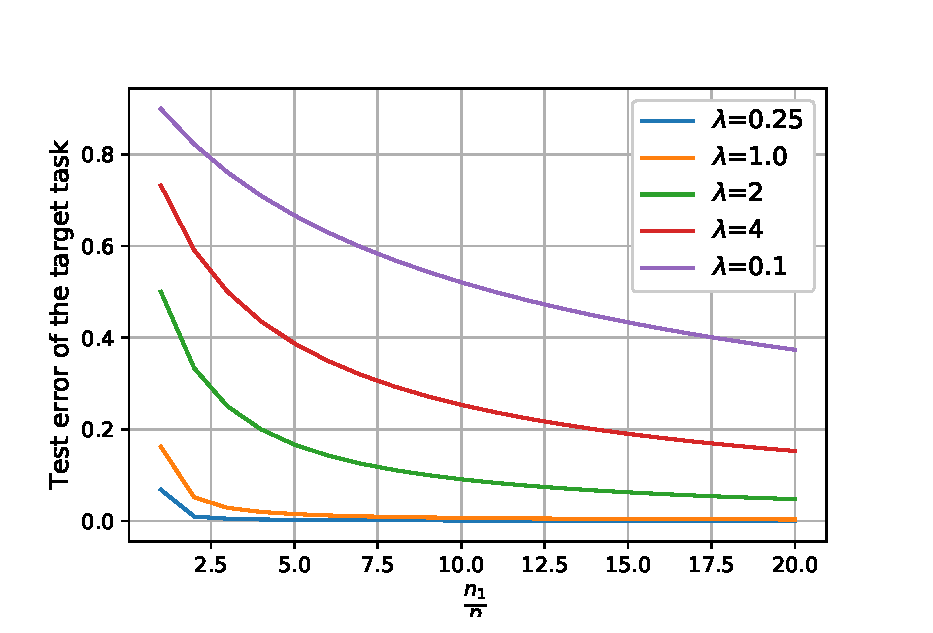
\includegraphics[width=0.9\textwidth]{figures/scaling.eps}
		\caption{When $\Sigma_1 = \Sigma_2 / \lambda$.}
		\label{fig_te_scaling}
	\end{minipage}\hfill
	\begin{minipage}{0.48\textwidth}
		\centering
		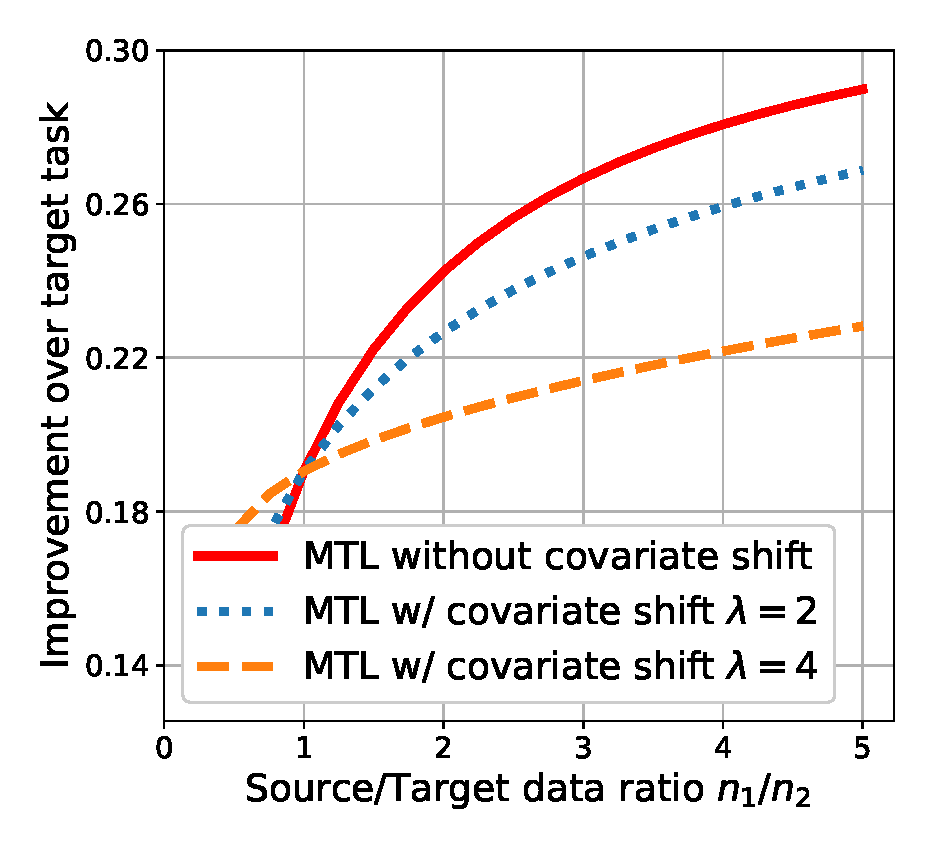
\includegraphics[width=0.9\textwidth]{figures/complementary.eps}
		\caption{When $\Sigma_1$ and $\Sigma_2$ are complementary. The number of target task data points is $n_2 = 4p$.}
		\label{fig_te_complement}
	\end{minipage}
\end{figure}


\paragraph{Extending the intuition to the general case.}
When there is model shift, i.e. $\beta_s = \beta_t$, we can still use Theorem \ref{thm_model_shift} (and Proposition \ref{prop_model_shift_tight}) to get the result.
\begin{itemize}
	\item \textbf{The effect of covariate shift:}
	\item \textbf{The effect of data ratio:}
\end{itemize}



%\section{Extensions to Multiple Tasks and Transfer Learning Settings}

Next, we describe our result for more than two tasks with same features, i.e. $X_i = X$ for any $i$.
This setting is prevalent in applications of multi-task learning to image classification, where there are multiple prediction labels/tasks for every image \cite{chexnet17,EA20}.
\begin{theorem}\label{thm_many_tasks}
%Suppose $X=Z\Sigma^{1/2}\in \R^{n\times p}$ satisfy Assumption \ref{assm_secA1} with $\rho:=n/p>1$ being some fixed constant. Consider data models  $Y_i = X\beta_i + \varepsilon_i$, $i=1,2,\cdots, t$, where $\e_i\in \R^{n}$ are random vectors with i.i.d. entries with mean zero, variance $\sigma^2$ and all moments as in \eqref{assmAhigh}. Moreover, assume that $X$, $\beta_i$ and $\e_i$ are all independent of each other.
	%Let $n = c \cdot p$.
	%Let $X\in\real^{n\times p}$ and $Y_i = X\beta_i + \varepsilon_i$, for $i = 1,\dots,k$.
	Consider $t$ data models $Y_i = X\beta_i + \varepsilon_i$, $i=1,2,\cdots, t$, where $X$ has covariance matrix $\Sigma$, and the entries of $\e_i$ are i.i.d. with mean zero and variance $\sigma^2$.
	%that satisfy Assumption \ref{assm_secA2} in the appendix.
	Let $U_r U_r^{\top}$ denote the best rank-$r$ subspace approximation of $(B^{\star})^\top\Sigma B^{\star}$, where $B^\star := [{\beta}_1,{\beta}_2,\dots,{\beta}_{t}]$ and $U_r\in\real^{t\times r}$. Suppose $(B^{\star})^\top\Sigma B^{\star}$ is of full rank in the sense that $\lambda_{\min}((B^{\star})^\top\Sigma B^{\star})\gtrsim \sigma^2$. Let $U_r(i)$ denote the $i$-th row vector of $U_r$.
	We have the following
	\squishlist
		\item $\te(\hat{\beta}_t^{\MTL}) < \te(\hat{\beta}_t^{\STL})$ with high probability if
		$$\left(1 - \norm{U_r(t)}^2 \right)\frac{\sigma^2}{\rho - 1} > \norm{\Sigma (B^{\star} U_r U_r(t) - \beta_t)}^2 +  \oo \left( \|B^\star\|^2 + \sigma^2\right).$$
		\item $\te(\hat{\beta}_t^{\MTL}) > \te(\hat{\beta}_t^{\STL})$ with high probability if
		$$\left(1 - \norm{U_r(t)}^2\right)\frac{\sigma^2}{\rho - 1} < \norm{\Sigma(B^{\star} U_r U_r(t) - \beta_t)}^2 -  \oo \left( \|B^\star\|^2 + \sigma^2\right).$$
	\squishend
\end{theorem}
%A similar result for the second setting can be found in Appendix \ref{app_proof_many_tasks}.


\section{Experiments}

\paragraph{A metric to determine when MTL performs better STL.}

\paragraph{When should we align task covariances in MTL.}
\begin{figure}
	\centering
	\includegraphics[width=0.5\textwidth]{figures/ratio_alignment_mr_sst_lstm.pdf}
	\caption{Covariate shift experiment.}
\end{figure}
\section{Related Work}


We refer the interested readers to several excellent surveys on multi-task and transfer learning for a comprehensive survey \cite{PY09,R17,ZY17,V20}.

\textit{Multi-task learning theory.}
Some of the earliest work on multi-task learning are Baxter \cite{B00}, Ben-David and Schuller \cite{BS03}.
Mauer \cite{M06} Generalization bounds for linear separation settings of MTL
Ben-David et al. \cite{BBCK10} provides uniform convergence bounds that combines empirical and target errors in an optimal way.
The benefit of learning multi-task representations is studied for learning certain half-spaces \cite{MPR16} and sparse regression \cite{LPTV09,LPVT11}.
Our work is closely related to Wu et al. \cite{WZR20}.
While Wu et al. provide generalization bounds to show that adding more labeled helps learn the target task more accurately, their results do not apply to explain the phenomena of negative transfer.

% Adding a regularization over $B$, e.g. .
\textit{Multi-task learning methodology.}
Ando and Zhang \cite{AZ05} introduces an alternating minimization framework for learning multiple tasks.
Argyriou et al. \cite{AEP08} presents a convex algorithm which learns common sparse representations across a pool of related tasks.
Evgeniou et al. \cite{EMP05} develops a framework for multi-task learning in the context of kernel methods.
\cite{KD12} observed that controlling the capacity can outperform the implicit capacity control of adding regularization over $B$.
The multi-task learning model that we have focused on is based on the idea of hard parameter sharing \cite{C93,R17}.
We believe that the technical tools we have developed can also be applied to many other multi-task learning models.

\textit{Random matrix theory.} The random matrix theory tool and related proof of this paper fall into a paradigm of the so-called local law of random matrices \cite{erdos2017dynamical}. For a sample covariance matrix $X^\top X$ with $\Sigma=\id$, such a local law was proved in \cite{isotropic}. It was later extended to sample covariance matrices with non-identity $\Sigma$ \cite{Anisotropic}, and separable covariance matrices \cite{yang2019spiked}. On the other hand, one may derive the asymptotic result in Theorem \ref{lem_cov_shift_informal} with error $\oo(1)$ using free addition of two independent random matrices in free probability theory \cite{nica2006lectures}. To the best of my knowledge, we do not find an {\it explicit result} for the sum of two sample covariance matrices with general covariates in the literature.



\section{Conclusions and Discussions}



\bibliographystyle{unsrt}
\bibliography{rf,ref_mtl}

\appendix
\textbf{Organizations.}
The appendix is organized as follows.
In Section \ref{app_proof_sec3}, we describe an extended background and a further reivew of related work.
In Section \ref{app_proof_main_thm}, we present the analysis of the bias-variance tradeoff for the case of two tasks.
In Section \ref{app_iso_cov}, we illustrate the above analysis in simplified settings including the isotropic model and covariate shifted settings without model distance.
In Section \ref{app_proof_many_tasks}, we extend our analysis to many tasks with the same features.
In Section \ref{sec_maintools}, we prove the bias and variance bounds used in the analysis.
Finally in Section \ref{app_experiments}, we fill in the missing details of our experiments.


\subsection{Limit of the Resolvent}\label{sec pf RMTlemma}

We now state the main random matrix result---Theorem \ref{main_cor}---which gives an almost optimal estimate on the resolvent $G(z)$ of $H$. It is conventionally called the {\it anisotropic local law} \cite{Anisotropic}. We define a domain of the spectral parameter $z$ as
\begin{equation}
\mathbf D:= \left\{z=E+ \ii \eta \in \C_+: |z|\le (\log n)^{-1} \right\}. \label{SSET1}
\end{equation}

\begin{theorem}\label{main_cor}
In the setting of Theorem \ref{thm_main_RMT}, let $q$ be equal to $n^{-\frac{\varphi - 4}{2\varphi}}$.
We have that the resolvent $G(z)$ converges to the matrix limit $\Gi(z)$:
for any deterministic unit vectors $\mathbf u, \mathbf v \in \mathbb R^{p+n_1+n_2}$, the following estimate \begin{equation}\label{aniso_law}
	\max_{z\in \mathbf D}\left| \mathbf u^\top (G(z)-\Gi(z)) \mathbf v \right|  \prec  q
\end{equation}
holds on the high probability event
\be\label{one_event}\left\{ \max_{1\le i\le n_1, 1\le j \le p}|Z^{(1)}_{i j}| \le (\log n) n^{\frac{2}{\varphi}}, \ \max_{1\le i\le n_2, 1\le j \le p}|Z^{(2)}_{i j}|\le (\log n) n^{\frac{2}{\varphi}} \right\}.\ee
\end{theorem}

The above result can be derived using the following lemma, which holds under a more general bounded support assumption on the random matrices.

\begin{lemma} \label{LEM_SMALL} %
In the setting of Theorem \ref{main_cor}, assume that $Z^{(1)}$ and $Z^{(2)}$ satisfy the bounded support condition \eqref{eq_support} with $Q=\sqrt{n}q = n^{ \frac{2}{\varphi}}$.
Then we have that the anisotropic local law in equation \eqref{aniso_law} holds 
for any deterministic unit vectors $\mathbf u, \mathbf v \in \mathbb R^{p+n_1+n_2}$.
\end{lemma}

\begin{remark}
The reason why we say the bounded support assumption is more general is because it provides greater flexibility in dealing with bounded moments. For example, we can also replace equation \eqref{Ptrunc} with
\begin{align*}
	\P\left(\max_{1\le i\le n, 1\le j \le p}|Z_{i j}|\ge n^{\frac{2}{\varphi}+\delta}\right) = \OO(  n^{-\varphi \delta}) 
	\end{align*}
	for a small constant $\delta>0$. Hence we can replace event \eqref{one_event} with 
	\be\nonumber \left\{ \max_{1\le i\le n, 1\le j \le p}|Z^{(1)}_{i j}| \le n^{\frac{2}{\varphi}+\delta}, \ \max_{1\le i\le n, 1\le j \le p}|Z^{(2)}_{i j}|\le   n^{\frac{2}{\varphi}+\delta} \right\},\ee
	which holds with higher probability. But on this event we need to take a larger $q=n^{-\frac{\varphi - 4}{2\varphi}+\delta}$, which means a worse convergence rate. In general, with Lemma \ref{LEM_SMALL} one can determine the most suitable trade-off between probability and convergence rate depending on one's need.
\end{remark}

Using the above result, we prove Theorem \ref{main_cor} using a simple cutoff argument.
\begin{proof}[Proof of Theorem \ref{main_cor}]%
We introduce the truncated matrices $\wt Z^{(1)}$ and $\wt Z^{(2)}$ with entries
$$ \wt Z^{(1)}_{\mu i}:= \mathbf 1\left( n^{-1/2}|Z^{(1)}_{\mu i}|\le q \log n \right)\cdot Z^{(1)}_{\mu i}, \quad \wt Z^{(2)}_{\nu i}:= \mathbf 1\left( n^{-1/2}|Z^{(2)}_{\nu i}|\le q \log n \right)\cdot Z^{(2)}_{\nu i}, $$
for $q= n^{-\frac{\varphi - 4}{2\varphi}}$. By equation \eqref{Ptrunc}, 
we have
\begin{equation}\label{XneX}
\mathbb P(\wt Z^{(1)} = Z^{(1)},  \wt Z^{(2)} = Z^{(2)}) =1-\OO ( (\log n)^{-\varphi}).
\end{equation}
By definition, we have 
\be\label{EwtZ}
\begin{split}
\E  \wt  Z^{(1)}_{\mu i} &= - \mathbb E \left[ \mathbf 1\left( |Z^{(1)}_{\mu i}|> qn^{1/2} \log n \right)Z^{(1)}_{\mu i}\right] ,\\ 
\E  |\wt  Z^{(1)}_{\mu i}|^2 &= 1 - \mathbb E \left[ \mathbf 1\left( |Z^{(1)}_{\mu i}|> qn^{1/2} \log n \right)|Z^{(1)}_{\mu i}|^2\right] .
\end{split}
\ee
Using the formula for expectation in terms of the tail probabilities, we can check that
\begin{align*}
&  \mathbb E \left| \mathbf 1\left( |Z^{(1)}_{\mu i}|> q n^{1/2}\log n \right)Z^{(1)}_{\mu i}\right| \\
= &\int_0^\infty \P\left( \left| \mathbf 1\left(  |Z^{(1)}_{\mu i}|> q n^{1/2}\log n \right)Z^{(1)}_{\mu i}\right| > s\right)\dd s \\
 = &\int_0^{qn^{1/2}\log n}\P\left( |Z^{(1)}_{\mu i}|> q  n^{1/2}\log n \right)\dd s +\int_{qn^{1/2}\log n}^\infty \P\left(|Z^{(1)}_{\mu i}| > s\right)\dd s  \\
\lesssim &\int_0^{qn^{1/2}\log n}\left(q  n^{1/2}\log n \right)^{-\varphi}\dd s +\int_{qn^{1/2}\log n}^\infty s^{-\varphi}\dd s \le n^{-2(\varphi-1)/\varphi},
\end{align*}
where in the third step we used the finite $\varphi$-th moment condition of $Z_{\mu i}^{(1)}$ %
and Markov's inequality. Similarly, we can obtain that
\begin{align*}
&  \mathbb E \left| \mathbf 1\left( |Z^{(1)}_{\mu i}|> qn^{1/2} \log n \right)Z^{(1)}_{\mu i}\right|^2 \\
= & 2\int_0^\infty s \P\left( \left| \mathbf 1\left( |Z^{(1)}_{\mu i}|> q n^{1/2}\log n \right)Z^{(1)}_{\mu i}\right| > s\right)\dd s \\
= & 2\int_0^{qn^{1/2}\log n} s \P\left( |Z^{(1)}_{\mu i}|> q  n^{1/2}\log n \right)\dd s +2\int_{qn^{1/2}\log n}^\infty s\P\left(|Z^{(1)}_{\mu i}| > s\right)\dd s  \\
\lesssim & \int_0^{qn^{1/2}\log n}s\left(q  n^{1/2}\log n \right)^{-\varphi}\dd s +\int_{qn^{1/2}\log n}^\infty s^{-\varphi+1}\dd s \le n^{-2(\varphi-2)/\varphi}.
\end{align*}
Plugging the above two estimates into equation \eqref{EwtZ} and using $\varphi>4$, we get that
\be\label{meanshif}
|\mathbb E  \wt  Z^{(1)}_{\mu i}| =\OO(n^{-3/2}), \quad  \mathbb E |\wt  Z^{(1)}_{\mu i}|^2 =1+ \OO(n^{-1}).
\ee
From the first estimate in equation \eqref{meanshif}, we can also get a bound on the operator norm:
\be\label{EZ norm}\|\E \wt Z^{(1)}\|=\OO(n^{-1/2}) .
\ee
Similar estimates also hold for $\wt Z^{(2)}$. 
Then we can centralize and rescale $\wt Z^{(1)}$ and $\wt Z^{(2)}$ as
$$ \wh Z^{(1)} :=\frac{\wt Z^{(1)} - \E \wt Z^{(1)} }{\left(\E|\wt Z^{(1)}_{\mu i}|^2\right)^{1/2}},\quad \wh Z^{(2)} :=\frac{\wt Z^{(2)} - \E \wt Z^{(2)} }{\left(\E|\wt Z^{(2)}_{\mu i}|^2\right)^{1/2}}.$$ 
Now $\wh Z^{(1)}$ and $\wh Z^{(2)}$ satisfy the assumptions of Lemma \ref{LEM_SMALL} with bounded support $\sqrt{n}q = n^{ \frac{2}{\varphi}}$, so we get that %
\be\label{GwhZZ}\left| \mathbf u^\top (G(\wh Z^{(1)},\wh Z^{(2)},z)-\Gi(z)) \mathbf v \right|  \prec  q,\ee
where $G(\wh Z^{(1)},\wh Z^{(2)},z)$ is defined in the same way as $G(z)$, but with $(Z^{(1)}, Z^{(2)})$ replaced by $(\wh Z^{(1)},\wh Z^{(2)})$.

Note that by equations \eqref{meanshif} and \eqref{EZ norm}, we can bound that for $k=1,2,$
$$ \|\wh Z^{(k)} - \wt Z^{(k)}\|\lesssim n^{-1}\|\wt Z^{(k)}\| + \|\E \wt Z^{(k)}\|\lesssim n^{-1/2}$$
with overwhelming probability, where we also used Fact \ref{fact_minv}(ii) to bound the operator norm of $\wt Z^{(k)}$. Together with estimate \eqref{priorim} below, this bound implies that %
$$\left| \mathbf u^\top (G(\wh Z^{(1)},\wh Z^{(2)},z)-G(Z^{(1)},Z^{(2)},z)) \mathbf v \right|  \lesssim  n^{-1/2}\|\wh Z^{(1)} - \wt Z^{(1)}\|+ n^{-1/2}\|\wh Z^{(2)} - \wt Z^{(2)}\|\lesssim n^{-1},$$
with overwhelming probability on the event $\{\wt Z^{(1)} = Z^{(1)},  \wt Z^{(2)} = Z^{(2)}\}$. Combining this estimate with equation \eqref{GwhZZ}, we obtain that estimate \eqref{aniso_law} holds for $G(z)$ on the event $\{\wt Z^{(1)} = Z^{(1)},  \wt Z^{(2)} = Z^{(2)}\}$, which concludes the proof by equation \eqref{XneX}.
\end{proof}


Now we are ready to complete the proof of Theorem \ref{thm_main_RMT} using Theorem \ref{main_cor}.

\begin{proof}[Proof of Theorem \ref{thm_main_RMT}, Part i)]
With the definition of matrix $W$ in equation \eqref{eigen2extra}, we can express $\Sigma^{(2)}\hat \Sigma^{-1}$ as
$$\Sigma^{(2)}\hat \Sigma^{-1} = n^{-1} ({\Sigma^{(2)}})^{1/2} V \cal G(0) V^{\top} ({\Sigma^{(2)}})^{-1/2},$$
where we recall that $\cal G(z)=(W-z\id )^{-1}$ is the resolvent of $W$.
Then by Theorem \ref{main_cor}, for any $1\le i \le p$ we have that
\begin{align}
& \left| \left[\Sigma^{(2)}\hat \Sigma^{-1} - n^{-1} (\Sigma^{(2)})^{1/2}V \Gi(0)V^\top(\Sigma^{(2)})^{-1/2} \right]_{ii}\right|  \nonumber\\
 = & n^{-1} \left|\mathbf e_i^\top (\Sigma^{(2)})^{1/2}V \left(\cal G(0)-\Gi(0)\right)V^\top (\Sigma^{(2)})^{-1/2} \mathbf e_i\right| \nonumber\\
\prec & n^{-1}q\|V^\top (\Sigma^{(2)})^{-1/2} \mathbf e_i\|\cdot \|V^\top (\Sigma^{(2)})^{1/2} \mathbf e_i\|   \lesssim n^{-1}q ,\label{G0Pi0}
\end{align}
on the event \eqref{one_event}, %
where $ q= n^{-\frac{\varphi - 4}{2\varphi}}$ and $\mathbf e_i$ denotes the standard basis vector along the $i$-th direction.
Next, we can verify that %
$$ n^{-1}  (\Sigma^{(2)})^{1/2}V \Gi(0)V^\top (\Sigma^{(2)})^{-1/2} = n^{-1}  \Sigma^{(2)}(a_1 \Sigma^{(1)}+  a_2\Sigma^{(2)})^{-1} .$$
Together with equation \eqref{G0Pi0}, this identity implies that %
\begin{align*}
 \tr \left[\Sigma^{(2)}\hat \Sigma^{-1} \right]& = \sum_{i=1}^p\left(\Sigma^{(2)}\hat \Sigma^{-1} \right)_{ii} = n^{-1}\tr \left[ \Sigma^{(2)}(a_1 \Sigma^{(1)}+  a_2\Sigma^{(2)})^{-1} \right] +\OO_\prec(q  ) 
 \end{align*}
on the event \eqref{one_event}, where we used Fact \ref{lem_stodomin} (i) in the second step. 
This concludes equation \eqref{lem_cov_shift_eq} using Definition \ref{stoch_domination} and the fact that $c_{\varphi}$ is any fixed value within $(0, \frac{\varphi - 4}{2\varphi})$.  %
\end{proof}
 

\begin{proof}[Proof of Theorem \ref{thm_main_RMT}, Part ii)]
Recall that in the setting of Theorem \ref{thm_main_RMT}, we have equation \eqref{calculate G'}.
For simplicity, we denote the vector $\bv:=V^\top  (\Sigma^{(2)})^{-1/2} \Sigma^{(1)}w$. 
By Corollary \ref{main_cor}, we have that
\be\nonumber 
\max_{z\in \C:|z|=(\log n)^{-1}}|\mathbf v^\top (G(z)-\Gi(z))\mathbf v| \prec q \|\mathbf v\|^2,%
\ee
on the event \eqref{one_event} with $ q:= n^{-\frac{\varphi - 4}{2\varphi}}$. Now combining this estimate with Cauchy's integral formula, we get that %
\be\label{apply derivlocal}
\begin{split}
  \bv^\top \cal G'(0)\bv  = \frac{1}{2\pi \ii}\oint_{\cal C} \frac{ \bv^\top \cal G(z)\bv }{z^2}\dd z &=  \frac{1}{2\pi \ii}\oint_{\cal C} \frac{ \bv^\top\Gi(z)\bv}{z^2}\dd z +\OO_\prec(q\|\mathbf v\|^2) \\
  &=  \bv^\top \Gi'(0)\bv + \OO_\prec(q\|\mathbf v\|^2),
\end{split}
\ee
where $\cal C$ is the contour $\{z\in \C: |z| = (\log n)^{-1} \}$. We can calculate the derivative $\bv^\top \Gi'(0)\bv$ as
\be\label{dervPi}
\bv^\top \Gi'(0)\bv = \bv^\top  \frac{a_3\Lambda^2+(1+a_4)\id_p}{(a_{1}\Lambda^2 + a_{2}\id_p)^2}\bv,
\ee
where we recall equation \eqref{cal G'0} and that $a_3 = - \frac{\dd a_1(0)}{\dd z}$ and $a_4 = - \frac{\dd a_2(0)}{\dd z}$. 
Taking the derivatives of the system of equations \eqref{selfomega_a}, we can derive equation \eqref{eq_a34extra} for $(a_3,a_4)$. This concludes the proof together with equation \eqref{apply derivlocal}.
\end{proof}



\subsection{Self-Consistent Equations}\label{sec contract}

The rest of this section is devoted to the proof of Lemma \ref{LEM_SMALL}. In this section, we show that the limiting equation \eqref{selfomega_a} has a unique solution $(a_1(z), a_2(z))$ for any $z\in \mathbf D$ in equation \eqref{SSET1}. Otherwise, Lemma \ref{LEM_SMALL} will be a vacuous statement. 


When $z=0$, the system of equations \eqref{selfomega_a} reduces to equation \eqref{eq_a12extra}, from which we can derive an equation of $a_1$ only:
\be\label{fa1}f(a_1)=\frac{n_1}{n_1 + n_2},\quad \text{with}\quad f(a_1):=a_1 +\frac{1}{n_1+n_2} \sum_{i=1}^p \frac{\lambda_i^2 a_1}{ \lambda_i^2 a_1+ (1- \frac{p}{n_1+n_2} - a_1) } .\ee
It is not hard to see that $f$ is strictly increasing on $[0,1-\frac{p}{n_1+n_2} ]$. Moreover, we have $f(0)=0<1$, $f(1-\frac{p}{n_1+n_2} )=1>\frac{n_1}{n_1+n_2}$, and $f(\frac{n_1}{n_1+n_2})>\frac{n_1}{n_1+n_2}$ if $\frac{n_1}{n_1+n_2}\le 1-\frac{p}{n_1+n_2}$. Hence by mean value theorem, there exists a unique solution $a_1$ satisfying
$$0< a_1 <\min\left(1-\frac{p}{n_1+n_2}, \frac{n_1}{n_1+n_2}\right).$$ 
Moreover, it is easy to check that $f'(x)=\OO(1)$ for $x\in [0, 1-\frac{p}{n_1+n_2}]$. Hence there exists a constant $\tau>0$, such that 
\be\label{a23}
\begin{split}
\frac{n_1}{n_1+n_2} \tau &\le   a_1 \le \min\left\{ 1-\frac{p}{n_1+n_2}  -\frac{n_1}{n_1+n_2}  \tau,\frac{n_1}{n_1+n_2} ( 1-\tau)\right\},\\ 
\tau & \le a_2\le 1 -\frac{p}{n_1+n_2}  - \frac{n_1}{n_1+n_2} \tau .
\end{split}
\ee 


Next, we prove the existence and uniqueness of the solution to the self-consistent equation \eqref{selfomega_a} for a general $z\in \mathbf D$.
We denote
\be\label{M1M2a1a2}
M_1(z):= -\frac{n_1+n_2}{n_1}a_1(z),\quad M_2(z):= -\frac{n_1+n_2}{n_2}a_2(z),
\ee
which are the asymptotic limits of $m_1(z)$ and $m_2(z)$ in equation \eqref{approximate m1m2}.
Then, it is not hard to verify that the system of equations \eqref{selfomega_a} can be rewritten as 
 the following system of equations:
\begin{equation}\label{selfomega}
\begin{split}
& \frac1{M_{1}} = \frac{\gamma_n}p\sum_{i=1}^p \frac{\lambda_i^2}{  z+\lambda_i^2 r_1 M_{1} +r_2 M_{2}  } - 1 ,\  \ \frac1{M_{2}} = \frac{\gamma_n}p\sum_{i=1}^p \frac{1 }{  z+\lambda_i^2 r_1 M_{1} +  r_2 M_{2}  }- 1 ,
\end{split}
\ee
where, for simplicity of notations, we introduced the following ratios 
\be\label{ratios}
 \gamma_n :=\frac{p}{n_1+n_2} ,\quad r_1 :=\frac{n_1}{n_1+n_2} ,\quad r_2 :=\frac{n_2}{n_1+n_2} .
\ee
One can compare equation \eqref{selfomega} for $(M_1(z),M_2(z))$ to equation \eqref{approximate m1m2} for $(m_1(z),m_2(z))$.
In the following proof, we shall focus on the system of equations \eqref{selfomega} because it is more suitable than equation \eqref{selfomega_a}  for our purpose of showing that $(m_1(z),m_2(z))$ converges to the asymptotic limit $(M_1(z),M_2(z))$.

Now we claim the following lemma, which gives the existence and uniqueness of the solution $(M_{1}(z),M_{2}(z))$ to the system of equations \eqref{selfomega}.

\begin{lemma} \label{lem_mbehaviorw}
There exist constants $c_0, C_0>0$ depending only on $\tau$ in Assumption \ref{assume_rm} and equation \eqref{a23} such that the following statements hold.
There exists a unique solution to equation \eqref{selfomega} under the conditions
\be\label{prior1}
|z|\le c_0, \quad  |M_{1}(z) - M_{1}(0)| + |M_{2}(z) - M_{2}(0)|\le c_0.
\ee
Moreover, the solution satisfies
\be\label{Lipomega}
 |M_{1}(z) - M_{1}(0)| + |M_2(z) - M_2(0)| \le C_0|z|.
\ee
\end{lemma}
 \begin{proof} %
 The proof is a standard application of the contraction principle. For reader's convenience, we give more details. First, it is easy to check that equation \eqref{selfomega} is equivalent to  
\begin{equation}\label{selfalter}
r_1M_{1}=-(1-\gamma_n) - r_2M_{2} - z\left( M_{2}^{-1}+1\right),\quad g_z(M_{2}(z))=1, 
\ee
where
$$g_z(M_{2}):= - M_{2} +\frac{\gamma_n}p\sum_{i=1}^p \frac{M_{2} }{  z -\lambda_i^2(1-\gamma_n)+ (1 - \lambda_i^2) r_2M_{2} - \lambda_i^2 z\left(  M_{2}^{-1}+1\right) }.$$
 We first show that there exists a unique solution $M_{2}(z)$ to the equation $g_z(M_{2}(z))=1$ under the conditions in equation \eqref{prior1}.
We abbreviate $\delta(z):= M_{2}(z) - M_{2}(0)$. From equation \eqref{selfalter}, we obtain that 
\begin{equation} \nonumber
0=\left[g_z(M_{2}(z)) -  g_0(M_{2}(0)) -g_z'(M_{2}(0))\delta(z)\right] + g_z'(M_{2}(0))\delta(z),
\ee
which gives that
\be\nonumber%
 \delta(z) =- \frac{ g_z(M_{2}(0)) - g_0(M_{2}(0)) }{g_z'(M_{2}(0))}- \frac{ g_z(M_{2}(0)+\delta(z)) -  g_z(M_{2}(0))-g_z'(M_{2}(0))\delta(z)}{g_z'(M_{2}(0))}.
 \ee
Inspired by this equation, we define iteratively a sequence ${\delta}^{(k)}(z) \in \C$ such that ${\delta}^{(0)}=0$, and 
\be\label{selfomega2}
 \delta^{(k+1)} =- \frac{g_z(M_{2}(0)) - g_0(M_{2}(0))}{g_z'(M_{2}(0))} -\frac{g_z(M_{2}(0)+ \delta^{(k)}) -  g_z(M_{2}(0))-g_z'(M_{2}(0))\delta^{(k)} }{g_z'(M_{2}(0))} .
 \ee
Then equation \eqref{selfomega2} defines a mapping $h_z:\C\to \C$, which maps $\delta^{(k)}$ to $\delta^{(k+1)}=h_z(\delta^{(k)})$.
 

With direct calculation, we obtain that
$$g_z'(M_{2}(0)) = -1 - \frac{\gamma_n}p\sum_{i=1}^p \frac{ \lambda_i^2(1-\gamma_n) - z\left[1- \lambda_i^2 \left(  2M_{2}^{-1}(0)+1\right)\right]  }{  \left[z -\lambda_i^2(1-\gamma_n)+ (1 - \lambda_i^2) r_2M_{2}(0) - \lambda_i^2 z\left( M_{2}^{-1}(0)+1\right)\right]^2 }.$$
Then it is not hard to check that there exist constants $\wt c, \wt C>0$ depending only on $\tau$ such that the following estimates hold: for all $z$, $\delta_1$ and $\delta_2$ such that $|z|\le \wt c$, $|\delta_1|  \le \wt c$ and $|\delta_2|  \le \wt c$,
\be\label{dust}
\left|\frac{1}{g_z'(M_{2}(0))} \right|\le \wt C, \quad   \left|\frac{g_z(M_{2}(0)) - g_0(M_{2}(0))}{g_z'(M_{2}(0))}\right|  \le \wt C|z| ,
\ee
and 
\be\label{dust222}
\left|\frac{g_z(M_{2}(0)+ \delta_1) -  g_z(M_{2}(0)+\delta_2)-g_z'(M_{2}(0))(\delta_1-\delta_2) }{g_z'(M_{2}(0))}\right|  \le \wt C|\delta_1-\delta_2|^2 .
\ee
Using equations \eqref{dust} and \eqref{dust222}, it is not hard to show that there exists a sufficiently small constant $c_1>0$ depending only on $\wt C$, such that 
$h_z: B_{d}  \to B_{d}$ is a self-mapping on the ball $B_d:=\{\delta \in \C: |\delta| \le d \}$, as long as $d\le c_1$ and $|z| \le c_1$. 
Now it suffices to prove that $h$ restricted to $B_d $ is a contraction, which then implies that ${\delta}:=\lim_{k\to\infty} { \delta}^{(k)}$ exists and $M_{2}(0)+\delta(z)$ is a unique solution to equation $g_z(M_{2}(z))=1$ subject to the condition $\|{\delta}\|_\infty \le d$. 


From the iteration relation \eqref{selfomega2}, using equation \eqref{dust222} one can readily check that
\be\label{k1k}
{ \delta}^{(k+1)} - { \delta}^{(k)}= h_z({\delta}^{(k)}) - h_z({\delta}^{(k-1)}) \le \wt C | { \delta}^{(k)}-{ \delta}^{(k-1)}|^2.
\ee
Hence as long as $d$ is chosen to be sufficiently small such that $2d\wt C\le 1/2$,  
then $h$ is indeed a contraction mapping on $ B_d$. This proves both the existence and uniqueness of the solution $M_{2}(z)=M_{2}(0)+\delta(z)$, if we choose $c_0$ in equation \eqref{prior1} as $c_0=\min\{c_1, d\}$. After obtaining $M_{2}(z)$, we can then find $M_{1}(z)$ using the first equation in \eqref{selfalter}. 

Note that with equation \eqref{dust} and ${\delta}^{(0)}= 0$, we can obtain from equation \eqref{selfomega2} that $ |{ \delta}^{(1)}(z)| \le \wt C|z| .$
With the contraction mapping, we have the bound 
\be\label{endalter}|{ \delta}| \le \sum_{k=0}^\infty |{  \delta}^{(k+1)}-{ \delta}^{(k)}| \le 2\wt C|z| \ \Rightarrow \ |M_{2}(z)-M_{2}(0)|\le 2\wt C|z| .\ee
Then using the first equation in equation \eqref{selfalter}, we immediately obtain the bound  $ r_1|M_{1}(z)-M_{1}(0)| \le C|z|$ for some constant $C>0$, which concludes equation \eqref{Lipomega} as long as if $r_1\gtrsim 1$. To deal with the $r_1=\oo(1)$ case, we go back to the first equation in \eqref{selfomega} and treat $M_{1}(z)$ as the solution to the following equation:
$$\wt g_z(M_{1}(z))=1,\quad \wt g_z(M_1):=- M_1 + \frac{\gamma_n}p\sum_{i=1}^p \frac{\lambda_i^2 M_1}{  z+\lambda_i^2 r_1 M_1 +r_2 M_{2}(z) }. $$
(Note that we have found the solution $M_2(z)$, so this is an equation of $M_1$ only.) 
Then with a similar argument as above (i.e. the proof between equation \eqref{selfalter} and equation \eqref{endalter}), we can conclude $|M_{2}(z)-M_{2}(0)|=\OO(|z|)$, which further concludes equation \eqref{Lipomega} together with equation \eqref{endalter}. 
We omit the details. %
\end{proof}

As a byproduct of the above contraction mapping argument, we also obtain the following stability result that will be used in the proof of Lemma \ref{LEM_SMALL}. Roughly speaking, it states that if  two complex functions $m_1(z)$ and $m_2(z)$ satisfy the self-consistent equation \eqref{selfomega} approximately up to some small errors, then $m_1(z)$ and $m_2(z)$ will be close to the solutions $M_1(z)$ and $M_2(z)$. Later this result will be applied to equation \eqref{approximate m1m2} to show that the averaged resolvents $m_1(z)$ and $m_2(z)$ indeed converge to $M_1(z)$ and $M_2(z)$, respectively.


\begin{lemma} \label{lem_stabw}
There exist constants $c_0, C_0>0$ depending only on $\tau$ in Assumption \ref{assume_rm} and equation \eqref{a23} such that the self-consistent equations in equation \eqref{selfomega} are stable in the following sense. Suppose $|z|\le c_0$, and $m_{1} $ and $m_{2} $ are analytic functions of $z$ such that
\be  \label{prior12}
|m_{1}(z) - M_{1}(0)| + |m_{2}(z) - M_2(0)|\le c_0.
\ee
Moreover, assume that $(m_1,m_2)$ satisfies the system of equations
\begin{equation}\label{selfomegaerror}
\begin{split}
&\frac{1}{m_{1}} + 1 -\frac{\gamma_n}p\sum_{i=1}^p \frac{\lambda_i^2}{  z+\lambda_i^2r_1m_{1} +r_2 m_{2}  } =\cal E_1,\ \ \frac{1}{m_{2}} + 1 -\frac{\gamma_n}p\sum_{i=1}^p \frac{1 }{  z+\lambda_i^2 r_1m_{1} +  r_2m_{2}  }=\cal E_2,
\end{split}
\ee
for some (deterministic or random) errors such that $  |\mathcal E_1| +  |\mathcal E_2| \le \theta(z),$ where $\theta(z)$ is a deterministic function of $z$ satisfying that $\theta(z) \le (\log n)^{-1}.$ Then we have 
 \begin{equation}
  \left|m_1(z)-M_{1}(z)\right| +  \left|m_2(z)-M_2(z)\right|\le C_0\delta(z).\label{Stability1}
\end{equation}
\end{lemma}



\begin{proof}%
Under condition \eqref{prior12}, we can obtain equation \eqref{selfalter} approximately up to some small error:
\be\label{selfalter2}r_1 m_{1}=-(1-\gamma_n) - r_2m_{2} - z\left(  {m_{2}^{-1}}+1\right) + \wt{\cal E}_1(z),\quad g_z(m_{2}(z))=1+ \wt{\cal E}_2(z),\ee
where the errors satisfy that $|\wt{\cal E}_1(z)|+ |\wt{\cal E}_2(z)|=\OO(\theta(z))$. Then we subtract equation \eqref{selfalter} from equation \eqref{selfalter2}, and consider the contraction principle for the function $\delta (z):= m_{2}(z) - M_2(z)$.  The rest of the proof is exactly the same as the one for Lemma \ref{lem_mbehaviorw}, so we omit the details.
\end{proof}





















\subsection{Beyond Multivariate Gaussian Matrices: an Anisotropic Local Law}\label{sec_Gauss}

 
In this section, we prove Lemma \ref{LEM_SMALL} by extending from the Gaussian random matrices to general random matrices.
The main difficulty in the proof is due to the fact that the entries of $Z^{(1)} U\Lambda$ and ${Z^{(2)}V}$ are not independent.
When the entries of $Z^{(1)}$ and $Z^{(2)}$ are sampled i.i.d. from an isotropic Gaussian distribution, $Z^{(1)} U$ and $Z^{(2)}V$ still obey the Gaussian distribution.
In this case, the problem is reduced to proving the anisotropic local law for $G(z)$ with $U=\id$ and $V=\id$, such that the entries of $ Z^{(1)} \Lambda  $ and ${Z^{(2)}}$ are independent.
For this case, we use the standard resolvent methods in \citet{isotropic,yang2019spiked,PY} and prove the following result.


\begin{proposition}\label{prop_diagonal}
 In the setting of Lemma \ref{LEM_SMALL}, assume further that the entries of $ Z^{(1)}$ and $ Z^{(2)}$ are i.i.d. Gaussian random variables. %
 Suppose $U$ and $V$ are identity.
	Then, the estimate \eqref{aniso_law} holds for all $z\in \mathbf D$ with $q= n^{-1/2}$.
\end{proposition}

 

Note that if the entries of $ Z^{(1)}$ and $ Z^{(2)}$ are Gaussian, then we have $\varphi=\infty$, which gives $q= n^{-\frac{\varphi - 4}{2\varphi}}=n^{-1/2}$.



Next we briefly describe how to extend Lemma \ref{LEM_SMALL} from the Gaussian case to the case with general $Z^{(1)}$ and $Z^{(2)}$ satisfying the bounded support condition (\ref{eq_support}) with $Q=\sqrt{n}q=n^{\frac{2}{\varphi}}$. 
With Proposition \ref{prop_diagonal}, it suffices is to prove that for $Z^{(1)}$ and $Z^{(2)}$ satisfying the assumptions in Lemma \ref{LEM_SMALL}, we have
\begin{equation*}%
 \left|\mathbf u^\top  \left( G(Z,z) -  G(Z^{\text{Gauss}}, z)\right) \mathbf v \right| \prec q 
\end{equation*}
for any deterministic unit vectors $\mathbf u,\mathbf v\in{\mathbb R}^{p+n_1+n_2}$ and $z\in \mathbf D$, where we abbreviated that 
$$Z:=\begin{pmatrix}Z^{(1)} \\ Z^{(2)}\end{pmatrix},\quad \text{and} \quad Z^{\text{Gauss}}:=\begin{pmatrix}(Z^{(1)})^{\text{Gauss}}\\ (Z^{(2)})^{\text{Gauss}}\end{pmatrix}.$$
We will prove the above statement using a continuous comparison argument developed in \citet{Anisotropic}. %
Since the proof is almost the same as the ones in Sections 7 and 8 of \citet{Anisotropic} and Section 6 of \citet{yang2019spiked}, we only describe the main ideas without writing down all the details.

We define the following continuous sequence of interpolating matrices between $Z^{\text{Gauss}}$ and $Z$. 

\begin{definition}[Interpolation]
We denote $Z^0:=Z^{\text{Gauss}}$ and $Z^1:=Z$. Let $\rho_{\mu i}^0$ and $\rho_{\mu i}^1$ be the laws of $Z_{\mu i}^0$ and $Z_{\mu i}^1$, respectively, for $i\in \cal I_0$ and $\mu \in \cal I_1\cup \cal I_2$. For any $\theta\in [0,1]$, we define the interpolated law
$\rho_{\mu i}^\theta := (1-\theta)\rho_{\mu i}^0+\theta\rho_{\mu i}^1.$ We shall work on the probability space consisting of triples $(Z^0,Z^\theta, Z^1)$ of independent $n\times p$ random matrices, where the matrix $Z^\theta=(Z_{\mu i}^\theta)$ has law
\begin{equation}\label{law_interpol}
\prod_{i\in \mathcal I_0}\prod_{\mu\in \mathcal I_1\cup \cal I_2} \rho_{\mu i}^\theta(\dd Z_{\mu i}^\theta).
\end{equation}
For $\lambda \in \mathbb R$, $i\in \mathcal I_0$ and $\mu\in \mathcal I_1\cup \cal I_2$, we define the matrix $Z_{(\mu i)}^{\theta,\lambda}$ through
\[\left(Z_{(\mu i)}^{\theta,\lambda}\right)_{\nu j}:=\begin{cases}Z_{\mu i}^{\theta}, &\text{ if }(j,\nu)\ne (i,\mu)\\ \lambda, &\text{ if }(j,\nu)=(i,\mu)\end{cases},\]
that is, it replaces the $(\mu,i)$-th entry of $Z^\theta$ with $\lambda$.
\end{definition}

\begin{proof}[Proof of Lemma \ref{LEM_SMALL}]
We shall prove %
equation \eqref{aniso_law} through interpolation matrices $Z^\theta$ between $Z^0$ and $Z^1$. We have seen that equation \eqref{aniso_law} holds for $G(Z^0,z)$ by Proposition \ref{prop_diagonal}. %
Using equation (\ref{law_interpol}) and fundamental calculus, we get the following basic interpolation formula:
for differentiable $F:\mathbb R^{n \times p}\rightarrow \mathbb C$,
\begin{equation}\label{basic_interp}
\frac{\dd}{\dd\theta}\mathbb E F(Z^\theta)=\sum_{i\in\mathcal I_0}\sum_{\mu\in\mathcal I_1\cup \cal I_2}\left[\mathbb E F\left(Z^{\theta,Z_{\mu i}^1}_{(\mu i)}\right)-\mathbb E F\left(Z^{\theta,Z_{\mu i}^0}_{(\mu i)}\right)\right],
\end{equation}
 provided all the expectations exist.
We shall apply equation \eqref{basic_interp} to the function $F(Z):=F_{\bu\mathbf v}^s(Z,z)$ for any fixed $s\in 2\N$, where %
\begin{equation*}%
 F_{\bu\mathbf v}(Z,z):=\left|\mathbf u^\top \left(G (Z,z)-\Gi(z)\right)\mathbf v\right|.
\end{equation*}
The main part of the proof is to show the following self-consistent estimate for the right-hand side of equation (\ref{basic_interp}): for any fixed $s\in 2\N$, any constant $\e>0$ and all $\theta\in[0,1]$,
 \begin{equation}\label{lemm_comp_4}
  \sum_{i\in\mathcal I_0}\sum_{\mu\in\mathcal I_1\cup \cal I_2}\left[\mathbb EF_{\bu\mathbf v}^s\left(Z^{\theta,Z_{\mu i}^1}_{(\mu i)},z\right)-\mathbb EF_{\bu\mathbf v}^s\left(Z^{\theta,Z_{\mu i}^0}_{(\mu i)},z\right)\right]\le (n^\e q)^{s}+C\E F_{\bu\mathbf v}^s\left(Z^{\theta},z\right) ,
 \end{equation}
 for some constant $C>0$. If equation \eqref{lemm_comp_4} holds, then combining equation \eqref{basic_interp} with  Gr\"onwall's inequality we obtain that for any fixed $s\in 2\N$ and constant $\e>0$, 
 $$\E\left|\bu^\top \left(G(Z^1,z)-\Pi(z)\right)\bv\right|^s  \lesssim (n^\e q)^{s}.$$
Finally applying Markov's inequality and noticing that $\e$ can be chosen arbitrarily small, we conclude equation \eqref{aniso_law}. 
Underlying the proof of the estimate (\ref{lemm_comp_4}) is an expansion approach, which is the same as the ones for Lemma 7.10 of \citet{Anisotropic} and Lemma 6.11 of \citet{yang2019spiked}. So we omit the details.
\end{proof}













\iffalse
This section is organized as follows. In Section \ref{sec tools}, we collect some basic estimates and resolvent identities that will be used in the proof of Lemma \ref{LEM_SMALL} and Proposition \ref{prop_diagonal}. Then in Section \ref{sec entry} we give the proof of Proposition \ref{prop_diagonal}, which concludes Lemma \ref{LEM_SMALL} when $Z^{(1)}$ and $Z^{(2)}$ have i.i.d. Gaussian entries. In Section \ref{sec_comparison}, we describe how to extend the result in Lemma \ref{LEM_SMALL} from the Gaussian case to the case where the entries of $Z^{(1)}$ and $Z^{(2)}$ are generally distributed. Finally, in Section \ref{sec contract}, we give the proof of Lemma \ref{lem_mbehaviorw} and Lemma \ref{lem_stabw}. In the proof, we always denote the spectral parameter by $z=E+\ii\eta$. 
\fi

Now it remains to prove Proposition \ref{prop_diagonal}, 
whose proof is based on the following entrywise local law. %
\begin{lemma}\label{prop_entry}
Under the assumptions of Proposition \ref{prop_diagonal}, %
the following estimate holds uniformly in $z\in \mathbf D$: %
\begin{equation}\label{entry_diagonal}
\max_{a,b\in \cal I}\left| G_{ab}(z)  - \Gi_{ab} (z) \right| \prec n^{-1/2}.
\end{equation} 
\end{lemma}


With Lemma \ref{prop_entry}, we can complete the proof of %
Proposition \ref{prop_diagonal}. %

\begin{proof}[Proof of Proposition \ref{prop_diagonal}]
With estimate (\ref{entry_diagonal}), one can use the polynomialization method in Section 5 of \citet{isotropic} to get the anisotropic local law (\ref{aniso_law}) with $q=n^{-1/2}$. The proof is exactly the same, except for some minor differences in notations. Hence we omit the details.
\end{proof}


\subsection{An Entrywise Local Law}\label{sec entry}
 
Finally, this subsection is devoted to the proof of Lemma \ref{prop_entry}. 
First, we claim the following a priori estimate on the resolvent $G(z)$ for $z\in \mathbf D$.

\begin{lemma}\label{lemm apri}
	In the setting of Lemma \ref{LEM_SMALL}, there exists a constant $C>0$ such that the following estimates hold uniformly in $z,z'\in \mathbf D$ with overwhelming probability:
\be\label{priorim}
\|G(z)\| \le C,%
\ee
and %
\be\label{priordiff} 
\left\|G  (z) - G(z')\right\| \le C|z-z'|.
\ee
\end{lemma}
\begin{proof}
 Our proof is a simple application of the spectral decomposition of $G$. Recall the matrix $\AF$ defined in equation \eqref{defn AF}. Let
\be\label{SVDW}
\AF= \sum_{k = 1}^{p} {\sqrt {\mu_k} \xi_k } \zeta _{k}^\top ,\quad \mu_1\ge \mu_2 \ge \cdots \ge \mu_{p} \ge 0 =\mu_{p+1} = \ldots = \mu_{n},\ee
be a singular value decomposition of $A$, where
$\{\xi_{k}\}_{k=1}^{p}$ are the left-singular vectors and $\{\zeta_{k}\}_{k=1}^{n}$ are the right-singular vectors.
Then using equation \eqref{green2}, we get that for $i,j\in \mathcal I_1$ and $\mu,\nu\in \mathcal I_1\cup \cal I_2$,
\be\label{spectral}
\begin{split}
& G_{ij} = \sum_{k = 1}^{p} \frac{\xi_k(i) \xi_k^\top(j)}{\mu_k-z}, \ \ G_{\mu\nu} =
z\sum_{k = 1}^{n} \frac{\zeta_k(\mu) \zeta_k^\top(\nu)}{\mu_k-z} , \ \ G_{i\mu} = G_{\mu i}= \sum_{k = 1}^{p} \frac{\sqrt{\mu_k}\xi_k(i) \zeta_k^\top(\mu)}{\mu_k-z}.
\end{split}
\ee
By Fact \ref{fact_minv} (ii), we have that with overwhelming probability
$\mu_p \ge \lambda_p(n^{-1}(Z^{(2)})^\top Z^{(2)}) \ge c_\tau $ for some constant $c_\tau>0$ depending only on $\tau$.  \HZ{to check} This further implies that
$$ \inf_{z\in \mathbf D}\min_{1\le k \le p}|\mu_k-z| \ge c_\tau - (\log n)^{-1}.$$
Combining this bound with equation \eqref{spectral}, we can easily conclude the estimates \eqref{priorim} and \eqref{priordiff}.
\end{proof}





















For the rest of this subsection, we present the proof of Lemma \ref{prop_entry}, which is the most technical part of the whole proof of Lemma \ref{LEM_SMALL}. 

\begin{proof}[Proof of Lemma \ref{prop_entry}]
Recall that under the assumptions of Lemma \ref{prop_entry},  we have %
\be\label{diagW}\AF \stackrel{d}{=} n^{-1/2}[\Lambda (Z^{(1)})^{\top}, (Z^{(2)})^\top],\ee
and it suffices to consider the resolvent in equation \eqref{resolv Gauss1} throughout the whole proof. 
The proof is divided into three steps. For simplicity, we introduce the following notation: for two (deterministic or random) nonnegative quantities $\xi$ and $\zeta$, 
we write $\xi\sim \zeta$ if $\xi\lesssim \zeta$ and $\zeta\lesssim \xi$.

\vspace{5pt}

\noindent{\bf Step 1: Large deviation estimates.} In this step, we prove some (almost) optimal large deviation estimates on the off-diagonal entries of $G$, and on the following $\cal Z$ variables. In analogy to Section 3 of \citet{EKYY1} and Section 5 of \citet{Anisotropic}, we introduce the $\cal Z$ variables  
\begin{equation*}
 \cal  Z_{{a}} :=(1-\mathbb E_{{a}})\left[\big(G_{{a}{a}}\big)^{-1}\right], %
\end{equation*}
where $\mathbb E_{{a}}[\cdot]:=\mathbb E[\cdot\mid H^{({a})}]$ denotes the partial expectation over the entries in the ${a}$-th row and column of $H$. Now using equation (\ref{resolvent2}), we get that for $i \in \cal I_0$, 
\begin{align}
\cal Z_i = & \frac{\lambda_i^2}{n} \sum_{\mu ,\nu\in \mathcal I_1}  G^{(i)}_{\mu\nu} \left(\delta_{\mu\nu} - Z^{(1)}_{\mu i}Z^{(1)}_{\nu i}\right)+\frac1n \sum_{\mu ,\nu\in \mathcal I_2}  G^{(i)}_{\mu\nu} \left( \delta_{\mu\nu} - Z^{(2)}_{\mu i}Z^{(2)}_{\nu i}\right) \nonumber\\
& - 2 \frac{\lambda_i}{n} \sum_{\mu\in \cal I_1,\nu\in \mathcal I_2} Z^{(1)}_{\mu i}Z^{(2)}_{\nu i}G^{\left( i \right)}_{\mu\nu},  \label{Zi}
\end{align}
and for $\mu\in \cal I_1$ and $\nu\in \cal I_2$, 
\begin{align}
&\cal  Z_\mu= \frac{1}{n} \sum_{i,j \in \mathcal I_0}  {\lambda_i \lambda_j}G^{(\mu)}_{ij} \left(\delta_{ij} - Z^{(1)}_{\mu i}Z^{(1)}_{\mu j}\right), \quad \cal Z_\nu = \frac{1}{n} \sum_{i,j \in \mathcal I_0} G^{(\nu)}_{ij} \left( \delta_{ij} - Z^{(2)}_{\nu i}Z^{(2)}_{\nu j}\right).\label{Zmu} 
\end{align}
Moreover, we introduce the random error
\begin{equation}  \label{eqn_randomerror}
 \Lambda _o : = %
 \max_{{a} \ne {b} } \left|  G_{{a}{a}}^{-1}G_{{a}{b}}   \right| ,
\end{equation}
which controls the size of the off-diagonal entries. The following lemma gives the desired large deviation estimate on $\Lambda_o$ and $\cal Z$ variables.

\begin{lemma}\label{Z_lemma}
Under the assumptions of Proposition \ref{prop_diagonal}, the following estimate holds uniformly in all $z\in \mathbf D$:
\begin{align}
\Lambda_o + \max_{{a}\in \cal I} |\cal Z_{{a}}|  \prec n^{-1/2}. \label{Zestimate1}
\end{align}
\end{lemma}
\begin{proof}
 Note that for any ${a}\in \cal I$, $H^{({a})}$ and $G^{({a})}$ also satisfies the assumptions in Lemma \ref{lemm apri}. Hence equations \eqref{priorim} and \eqref{priordiff} also hold for $G^{({a})}$ with overwhelming probability. Now applying equations \eqref{eq largedev1} and \eqref{eq largedev2} to equation (\ref{Zi}), %
we get that for any $i\in \cal I_0$, %
\begin{equation}\nonumber%
\begin{split}
\left| \cal Z_{i}\right|&\lesssim \frac{1}{n} \left|\sum_{\mu ,\nu\in \mathcal I_1}  G^{(i)}_{\mu\nu} \left(\delta_{\mu\nu} - Z^{(1)}_{\mu i}Z^{(1)}_{\nu i}\right)\right|+\frac1n \left|\sum_{\mu ,\nu\in \mathcal I_2}  G^{(i)}_{\mu\nu} \left( \delta_{\mu\nu} - Z^{(2)}_{\mu i}Z^{(2)}_{\nu i}\right)\right| + \frac{1}{n} \left|\sum_{\mu\in \cal I_1,\nu\in \mathcal I_2} Z^{(1)}_{\mu i}Z^{(2)}_{\nu i}G^{\left( i \right)}_{\mu\nu}\right| \\
&\prec  \frac{1}{n} \left( \sum_{\mu,\nu \in \cal I_1\cup \cal I_2 }  {| G_{\mu\nu}^{(i)}|^2 }  \right)^{1/2} \prec n^{-1/2} .
\end{split}
\end{equation}
Here in the last step we used equation \eqref{priorim} to get that for any $\mu\in \cal I_1\cup \cal I_2$,
\be\label{GG*}\sum_{\nu \in \cal I_1\cup \cal I_2 }  | G_{\mu\nu}^{(i)} |^2\le \sum_{{a} \in \cal I } | G_{\mu{a}}^{(i)} |^2 =\left[G^{(i)}(G^{(i)})^* \right]_{\mu\mu} =\OO(1),\quad \text{with overwhelming probability,}\ee
where $(G^{(i)})^*$ denotes the complex conjugate transpose of $G^{(i)}$. Similarly, applying equations \eqref{eq largedev1} and \eqref{eq largedev2} to $\cal Z_{\mu}$ and $\cal Z_\nu$ in equation (\ref{Zmu}) and using equation \eqref{priorim}, we can obtain the same bound.

Next we prove the off-diagonal estimate on $\Lambda_o$. For $i\in \mathcal I_1$ and ${a}\in \cal I\setminus \{i\}$, using equations \eqref{resolvent3}, \eqref{eq largedev1} and \eqref{priorim}, we can obtain that 
\begin{align*}
  \left|G_{ii}^{-1}G_{i{a}}\right| &\le {n^{-1/2}}\left|  {\lambda_i}\sum_{\mu \in \cal I_1} Z^{(1)}_{\mu i} G^{(i)}_{\mu a}(z)\right| + n^{-1/2}\left|\sum_{\mu \in \cal I_2} Z^{(2)}_{\mu i} G^{(i)}_{\mu a}(z)  \right| \\
& \prec  n^{-1/2}\left( \sum_{\mu \in \cal I_1\cup \cal I_2}  {| G_{\mu {a}}^{(i)} |^2 }  \right)^{1/2} \prec n^{-1/2}. 
 \end{align*}
 We can get the same estimate for $\left|G_{\mu\mu}^{-1} G_{\mu{b}} \right|$, $\mu \in \mathcal I_1\cup \cal I_2$ and ${b}\in \cal I\setminus \{ \mu\}$, using a similar argument.  
Thus we obtain that $\Lambda_o\prec n^{-1/2}$. %
\end{proof}

Note that combining $\max_a|G_{aa}|=\OO(1)$ by equation \eqref{priorim} with equation \eqref{Zestimate1}, we immediately conclude equation \eqref{entry_diagonal} for the off-diagonal entries with ${a}\ne {b}$.



\vspace{5pt}

\noindent{\bf Step 2: Self-consistent equations.} 
In this step, we derive the approximate self-consistent equations in \eqref{approximate m1m2} satisfied by $m_1(z)$ and $m_2(z)$ with more precise error rates. %
More precisely, we will show that $(m_1(z),m_2(z))$ satisfies equation \eqref{selfomegaerror} for some small errors satisfying $|\cal E_{1}|+ |\cal E_{2}|\prec n^{-1/2}$. Later in Step 3, we will apply Lemma \ref{lem_stabw} to show that $(m_1(z),m_2(z))$ is close to $(M_{1}(z),M_{2}(z))$. %

We define the following $z$-dependent event 
\be\label{Xiz}\Xi(z):=\left\{ |m_{1}(z)-M_{1}(z)| + |m_{2}(z)-M_{2}(z)| \le (\log n)^{-1/2}\right\}.\ee
Note that by equation \eqref{Lipomega}, we have that for $z\in \mathbf D$ the following estimates hold:
$$|M_{1}(z)-M_1(0)|=|M_{1}(z)+r_1^{-1}a_1|\lesssim (\log n)^{-1},\quad |M_{2}(z)+M_2(0)|=|M_{2}+r_2^{-1}a_2|\lesssim (\log n)^{-1}.$$
Together with the estimates in equation \eqref{a23} and the assumption that the singular values $\lambda_i$ are bounded, we obtain the following estimates
\be\label{Gsim1}
 |M_{1}| \sim |M_{2}| \sim 1, \quad |z+\lambda_i^2 r_1M_{1} + r_2 M_{2}|\sim 1,\quad \text{uniformly in $z\in \mathbf D$}  . \ee
 Moreover, using equation \eqref{selfomega} we get
 \be\label{Gsim0}
 \quad \left|1 + \gamma_n M(z)\right| = |M_2^{-1}(z)| \sim 1, \quad  |1+\gamma_n M_{0}(z)| = |M_1^{-1}(z)| \sim 1  ,
\ee
 uniformly in $z\in \mathbf D$, where we abbreviated
 \be\label{defn mc1c}M(z):=-\frac1p\sum_{i=1}^p\frac{1}{z+\lambda_i^2 r_1M_{1}(z) +r_2M_{2}(z)},\quad M_{0}(z):=-\frac1p\sum_{i=1}^p\frac{\lambda_i^2}{z+\lambda_i^2 r_1M_{1}(z) +r_2M_{2}(z)}. \ee
In fact, $M(z)$ and $M_0(z)$ are the asymptotic limits of $m(z)$ and $m_0(z)$, respectively. Plugging equation \eqref{Gsim1} into equation \eqref{defn_piw}, we get that
\be
|\Gi_{{a}{a}}(z)| \sim 1 \ \ \text{uniformly in } z\in \mathbf D \ \text{ and } \ {a}\in \cal I.
\ee 
Then we prove the following key lemma, which shows that $(m_1(z),m_2(z))$ satisfies equation \eqref{selfomegaerror} with some small errors $\cal E_{1}$ and $\cal E_{2}$.

\begin{lemma}\label{lemm_selfcons_weak}
Under the assumptions of Proposition \ref{prop_diagonal}, the following estimates hold uniformly in $z \in \mathbf D$: 
\begin{equation} \label{selfcons_lemm}
{\mathbf 1}(\Xi) \left|\frac{1}{m_{1}} + 1 -\frac{\gamma_n}p\sum_{i=1}^p \frac{\lambda_i^2}{  z+\lambda_i^2r_1m_{1} + r_2m_{2}  } \right|\prec n^{-1/2},\ee
and
\begin{equation} \label{selfcons_lemm2}
  {\mathbf 1}(\Xi)\left|\frac{1}{m_{2}} + 1 -\frac{\gamma_n}p\sum_{i=1}^p \frac{1 }{  z+\lambda_i^2 r_1m_{1} +  r_2m_{2}  }\right|\prec n^{-1/2}.
\ee
\end{lemma}

\begin{proof}
By equations (\ref{resolvent2}), (\ref{Zi}) and (\ref{Zmu}), we obtain that %
\begin{align}
\frac{1}{{G_{ii} }}&=  - z - \frac{\lambda_i^2}{n} \sum_{\mu\in \mathcal I_1} G^{\left( i \right)}_{\mu\mu}- \frac{1}{n} \sum_{\mu\in \mathcal I_2} G^{\left( i \right)}_{\mu\mu} + \cal Z_i =  - z - \lambda_i^2 r_1m_1 - r_2m_2 + \cal E_i, \quad \text{for }i \in \cal I_0, \label{self_Gii}\\
\frac{1}{{G_{\mu\mu} }}&=  - 1 - \frac{1}{n} \sum_{i\in \mathcal I_0}\lambda_i^2 G^{\left(\mu\right)}_{ii}+ \cal Z_{\mu} =  - 1  - \gamma_n m_0 + \cal E_\mu, \quad \text{for }\mu \in \cal I_1,  \label{self_Gmu1}\\
\frac{1}{{G_{\nu\nu} }}&=  - 1 - \frac{1}{n} \sum_{i\in \mathcal I_0} G^{\left(\nu\right)}_{ii}+\cal Z_{\nu} =   - 1 - \gamma_n m + \cal E_\nu, \quad \text{for }\nu \in \cal I_2, \label{self_Gmu2}
\end{align}
where we denoted (recall equation \eqref{defm} and Definition \ref{defn_Minor}) %
$$\cal E_i :=\cal Z_i + \lambda_i^2 r_1\left(m_1 - m_1^{(i)}\right) + r_2\left(m_2-m_2^{(i)}\right) ,$$
and
$$\cal E_\mu :=\cal Z_{\mu} + \gamma_n(m_0-m_0^{(\mu)}),\quad \cal E_\nu:=\cal Z_{\nu} +\gamma_n(m-m^{(\nu)}) .$$
Using equations (\ref{resolvent8}), \eqref{eqn_randomerror} and (\ref{Zestimate1}), we can bound that  
\begin{equation}\nonumber
  |m_1 - m_1^{(i)}| \le   \frac1{n_1}\sum_{\mu\in \mathcal I_1}  \left|\frac{G_{\mu i} G_{i\mu}}{G_{ii}}\right| \le |\Lambda_o|^2|G_{ii}| \prec n^{-1}.
\end{equation}
where we also used bound \eqref{priorim} in the last step. Similarly, we also have that 
\be \nonumber%
 |m_2 - m_2^{(i)}| \prec n^{-1} , \quad |m_0 - m_0^{(\mu)}| \prec n^{-1},\quad  |m-m^{(\nu)}| \prec n^{-1},  \ee
for any $i\in \cal I_0$, $\mu \in \cal I_{1}$ and $\nu\in \cal I_2$. Together with equation (\ref{Zestimate1}), we obtain the bound %
\begin{equation}\label{erri}
\max_{i\in \cal I_0} |\cal E_i | +\max_{\mu \in \cal I_1\cup \cal I_2} |\cal E_\mu|  \prec n^{-1/2}.
\end{equation}

 With equation \eqref{Gsim1} and the definition of the event $\Xi$ in \eqref{Xiz}, we get that 
 $$\mathbf 1(\Xi)|z + \lambda_i^2 r_1m_1+r_2m_2|\sim1.$$ 
 Combining it with equations (\ref{self_Gii}) and \eqref{erri}, we obtain that
\be\label{Gmumu0}
\mathbf 1(\Xi)G_{ii}=\mathbf 1(\Xi)\left[-\frac{1}{z + \lambda_i^2 r_1 m_1+r_2 m_2} +\OO_\prec\left(n^{-1/2}\right)\right].
\ee
Plugging \eqref{Gmumu0} into the definitions of $m$ and $m_0$ in equation \eqref{defm}, we get
\begin{align}
\mathbf 1(\Xi)m&=\mathbf 1(\Xi)\left[-\frac1p\sum_{i\in \cal I_0}\frac{1}{z + \lambda_i^2 r_1 m_1+r_2 m_2}  +\OO_\prec\left(n^{-1/2}\right)\right],\label{Gmumu} \\
\mathbf 1(\Xi)m_0&=\mathbf 1(\Xi)\left[-\frac1p\sum_{i\in \cal I_0}\frac{\lambda_i^2}{z + \lambda_i^2 r_1 m_1+r_2 m_2}   +\OO_\prec\left(n^{-1/2}\right)\right]. \label{Gmumu2}
\end{align}
As a byproduct, we obtain from these two equations and equation \eqref{defn mc1c} that  
\be\label{Gsim11}
 |m(z)-M(z)| +|m_0(z)-M_{0}(z)|  \lesssim (\log n)^{-1/2}, \quad \text{with overwhelming probability on } \Xi. 
\ee
Together with equation \eqref{Gsim0}, we get that %
\be\label{Gsim2}
|1+\gamma_nm (z)|\sim 1, \quad |1+\gamma_nm_0(z)|\sim 1, \quad \text{with overwhelming probability on } \Xi.
\ee
Now combining equations \eqref{self_Gmu1}, \eqref{self_Gmu2}, \eqref{erri} and  \eqref{Gsim2}, we obtain that for $\mu \in \cal I_1$ and $\nu \in \cal I_2,$ %
\begin{align}\label{Gii0} 
&\mathbf 1(\Xi)\left(G_{\mu\mu}+\frac{1}{1 + \gamma_nm_0}\right)  \prec n^{-1/2}  , \quad \mathbf 1(\Xi)\left(G_{\nu\nu}+\frac{1}{1 + \gamma_nm}\right) \prec n^{-1/2}  .
\end{align}
Taking average over $\mu\in \cal I_1$ and $\nu\in \cal I_2$, we get that %
\begin{align}\label{Gii000}
& \mathbf 1(\Xi)\left(m_1+\frac{1}{1 + \gamma_n m_0}\right) \prec n^{-1/2}  ,\quad  \mathbf 1(\Xi)\left(m_2+\frac{1}{1 +\gamma_n  m}\right) \prec n^{-1/2}  ,
\end{align}
which further implies
\be\label{Gii}
 \mathbf 1(\Xi)\left(\frac{1}{m_1} + 1 + \gamma_nm_0\right) \prec  n^{-1/2} ,\quad \mathbf 1(\Xi)\left(\frac{1}{m_2} + 1 + \gamma_nm\right) \prec  n^{-1/2} .
\ee
Finally, plugging equations \eqref{Gmumu} and \eqref{Gmumu2} into equation \eqref{Gii}, we conclude equations (\ref{selfcons_lemm}) and (\ref{selfcons_lemm2}). 
\end{proof}



\noindent{\bf Step 3: $\Xi$ holds with overwhelming probability.} In this step, we show that the event $\Xi(z)$ in \eqref{Xiz} actually holds with overwhelming probability for all $z\in \mathbf D$. Once we have proved this fact, applying Lemma \ref{lem_stabw} to equations \eqref{selfcons_lemm} and  \eqref{selfcons_lemm2} immediately shows that $(m_1(z),m_2(z))$ is close to $(M_{1}(z),M_{2}(z))$ up to an error of order $\OO_\prec(n^{-1/2})$. 

We claim that it suffices to show that
\be\label{Xiz0}
|m_{1}(0)-M_{1}(0)| + |m_{2}(0)-M_{2}(0)| \prec n^{-1/2}.
\ee
 In fact, notice that by equations \eqref{Lipomega} and \eqref{priordiff} we have
$$ |M_{1}(z)-M_{1}(0)|+|M_2(z)-M_2(0)|=\OO((\log n)^{-1}),\quad  |m_{1}(z)-m_{1}(0)|+ |m_{2}(z)-m_{2}(0)|=\OO((\log n)^{-1}),$$ 
with overwhelming probability for all $z\in \mathbf D$. Thus if equation \eqref{Xiz0} holds, we can obtain that 
\be\label{roughh1} 
\sup_{z\in \mathbf D} \left(|m_{1}(z)-M_{1}(z)| + |m_{2}(z)-M_{2}(z)|\right)  \lesssim (\log n)^{-1} \quad \text{with overwhelming probability},\ee
and %
\be\label{roughh2} \sup_{z\in \mathbf D} \left( |m_{1}(z)-M_{1}(0)|+ |m_{2}(z)-M_{2}(0)|\right) \lesssim (\log n)^{-1} \quad \text{with overwhelming probability}.\ee
The equation \eqref{roughh1} shows that $\Xi$ holds with overwhelming probability, while the equation \eqref{roughh2} verifies the condition \eqref{prior12} of Lemma \ref{lem_stabw}. Now applying Lemma \ref{lem_stabw} to equations \eqref{selfcons_lemm} and \eqref{selfcons_lemm2}, we obtain that
\be\label{Xizz}
|m_{1}(z)-M_{1}(z)|+ |m_{2}(z)-M_2(z)| \prec n^{-1/2} 
\ee
uniformly for all $z\in \mathbf D$. Together with equations \eqref{Gii0} and \eqref{Gii000}, equation \eqref{Xizz} implies that
\be\label{Xizz2} \max_{\mu\in \cal I_1} |G_{\mu\mu}(z)-M_{1}(z)|+ \max_{\nu\in \cal I_2} |G_{\nu\nu}(z)-M_{2}(z)|\prec n^{-1/2}.
\ee
Then plugging estimate \eqref{Xizz} into equation \eqref{Gmumu0} and recalling \eqref{M1M2a1a2}, we obtain that 
$$\max_{{i}\in \cal I_1}|G_{ii}(z)-\Gi_{ii}(z)| \prec n^{-1/2}. 
$$
Together with equation \eqref{Xizz2}, it gives the diagonal estimate
\be\label{diagest}
\max_{{a}\in \cal I}|G_{{a}{a}}(z)-\Pi_{{a}{a}}(z)| \prec n^{-1/2}. 
\ee
Combining equation \eqref{diagest} with the off-diagonal estimate on $\Lambda_o$ in equation \eqref{Zestimate1}, we conclude the proof of Lemma \ref{prop_entry}. 

Finally, we give the proof of equation \eqref{Xiz0}.
By equation \eqref{spectral}, we have that with overwhelming probability,
$$ m(0)=\frac1p\sum_{i\in \cal I_0}G_{ii}(0) = \frac1p\sum_{i\in \cal I_0}\sum_{k = 1}^{p} \frac{|\xi_k(i)|^2 }{\mu_k} \ge \mu_1^{-1} \gtrsim 1,$$
where we used Fact \ref{fact_minv} in the last step to bound  $\mu_1 \ge \lambda_1(n^{-1}(Z^{(2)})^\top Z^{(2)}) \gtrsim 1$ with overwhelming probability. \HZ{to check}
Similarly, we can also get that $m_0(0)$ is positive and has size $m_0(0)\sim 1$. Hence we have the estimates
\be\label{add_1+m}1+\gamma_n m(0)\sim 1,\quad 1+\gamma_n m_0(0)\sim 1.\ee
Combining these estimates with equations \eqref{self_Gmu1}, \eqref{self_Gmu2} and  \eqref{erri}, we obtain that equation \eqref{Gii000} holds at $z=0$ even without the indicator function $\mathbf 1(\Xi)$. Furthermore, we have that with overwhelming probability,
$$  \left|\lambda_i^2 r_1m_1(0)+r_2m_2(0)\right|=\left|\frac{\lambda_i^2 r_1}{ 1+\gamma_n m_0(0)} +\frac{r_2}{1+\gamma_n m(0)}+ \OO_\prec (n^{-1/2})\right| \sim 1 .$$
 Then combining this estimate with equations (\ref{self_Gii}) and \eqref{erri}, we obtain that equations \eqref{Gmumu} and \eqref{Gmumu2} also hold at $z=0$ even without the indicator function $\mathbf 1(\Xi)$. Finally, plugging equations \eqref{Gmumu} and \eqref{Gmumu2} into equation \eqref{Gii}, we conclude that equations \eqref{selfcons_lemm} and  \eqref{selfcons_lemm2}  hold at $z=0$, that is,
\begin{equation} \label{selfcons_lemma222}
\begin{split}
& \left|\frac{1}{m_{1}(0)} + 1 -\frac1n\sum_{i=1}^p \frac{\lambda_i^2}{ \lambda_i^2r_1m_{1}(0) + r_2m_{2}(0)  } \right|\prec n^{-1/2},\\ 
&\left|\frac{1}{m_{2}(0)} + 1 -\frac1n\sum_{i=1}^p \frac{1 }{ \lambda_i^2 r_1m_{1}(0) + r_2 m_{2}(0)  }\right|\prec n^{-1/2}.
\end{split}
\ee

Denoting $y_{1}=-m_{1}(0)$ and $y_{2}=-m_{2}(0)$, by equation \eqref{Gii000} we have
$$y_1= \frac{1}{1+\gamma_n m_{0}(0)} +\OO_\prec(n^{-1/2}),\quad y_2= \frac{1}{1+\gamma_n m(0)}+\OO_\prec(n^{-1/2}).$$ 
Hence by \eqref{add_1+m}, there exists a constant $c>0$ such that 
\be\label{omega12} c \le y_1 \le 1, \quad  c\le y_2\le 1, \quad \text{with overwhelming probability}.\ee
Also one can verify from equation \eqref{selfcons_lemma222} that $(r_1y_1,r_2y_2)$ satisfies approximately the same system of equations as equation \eqref{eq_a12extra}:
\be\label{selfcons_lemm000}
r_1y_1+r_2 y_2 = 1-\gamma_n + \OO_\prec (n^{-1/2}),\quad r_1^{-1}f(r_1y_1)=1 + \OO_\prec (n^{-1/2}),
\ee
where recall that the function $f$ was defined in equation \eqref{fa1}. The first equation of \eqref{selfcons_lemm000} and equation \eqref{omega12} together imply that $y_1 \in [0,r_1^{-1}(1-\gamma_n)]$ with overwhelming probability. For the second equation of \eqref{selfcons_lemm000}, we know that $y_1=r_1^{-1}a_1$ is a solution. Moreover, it is easy to check that the function $g(y_1):= r_1^{-1}f(r_1y_1)$ is strictly increasing and has bounded derivative on $[0,r_1^{-1}(1-\gamma_n)]$. So by basic calculus, %
we obtain that 
$$|m_1(0)-M_1(0)|=|y_1-r_1^{-1}a_1|\prec n^{-1/2}.$$ 
Plugging it into the first equation of equation \eqref{selfcons_lemm000}, we get 
$$|m_2(0)-M_2(0)|=|y_2-r_2^{-1}a_2|\prec n^{-1/2}.$$ The above two estimates conclude equation \eqref{Xiz0}.
\end{proof}









\iffalse
In random matrix theory, it is much more convenient to consider matrices $n^{-1/2}Z^{(1)}$ and $n^{-1/2}Z^{(2)}$ with an extra $n^{-1/2}$ factor, where we denote $n:=n_1+n_2$.
The advantage of this scaling is that the singular eigenvalues of $n^{-1/2}Z^{(1)}$ and $n^{-1/2}Z^{(2)}$ all lie in a bounded support that does not grow with $n$. For reader's convenience, we first state the exact properties (some of which have already been stated in words in Section \ref{sec_prelim}) that we shall need for the results and proofs in this section. %


We have assumed that $Z^{(1)}$ and $Z^{(2)}$ are $n_1\times p$ and $n_2\times p$ random matrices with i.i.d. entries satisfying
\begin{equation}\label{assm1}
\mathbb{E} (Z^{(1)})_{11} =\mathbb{E} (Z^{(2)})_{11} =0, \ \quad \ \mathbb{E} \vert (Z^{(1)})_{11} \vert^2=\mathbb{E} \vert (Z^{(2)})_{11} \vert^2  =1.
\end{equation}
Recall that we have defined $\rho_1= n_1/p$ and $\rho_2=n_2/p$ in introduction. We assume that they satisfy
\be\label{assm2}
0\le \rho_1 \le \tau^{-1}, \quad 1+\tau \le \rho_{2} \le \tau^{-1},
\ee
for a small constant $0<\tau<1$.
\fi


 \iffalse
We assume that $\Sig_1$ and $\Sig_2$ have eigendecompositions
\be\label{eigen}\Sig_1= Q_1\Lambda_1 Q_1^\top, \ \ \Sig_2= Q_2\Lambda_2 Q_2^\top,\ \ \Lambda_1=\text{diag}(\lambda_1^{(1)}, \ldots, \lambda^{(1)}_p), \ \ \Lambda_2=\text{diag}( \lambda^{(2)}_1, \ldots, \lambda^{(2)}_p),
\ee
where the eigenvalues satisfy that
\begin{equation}\label{assm3}
\tau \le \lambda^{(1)}_p \le \ldots \le \lambda^{(1)}_2  \le \lambda^{(1)}_1 \le \tau^{-1}, \quad \tau \le   \lambda^{(2)}_p \le \ldots \le \lambda^{(2)}_2 \le \lambda^{(2)}_1 \le \tau^{-1}.
\ee


We assume that $M=\Sig_1^{1/2} \Sig_2^{-1/2}$ has a singular value decomposition \eqref{eigen2} .....
\be%
M= U\Lambda V^\top, \quad \Lambda=\text{diag}( \lambda_1, \ldots, \lambda_p),
\ee
where by equation \eqref{assm3} we have %
\begin{equation}\label{assm32}
\tau \le \lambda_p \le \lambda_1 \le \tau^{-1} .%
\end{equation}
\fi




\iffalse
Before entering into the formal proof, we state two preparation lemmas, both of which have been used crucially in some previous proofs. First, for $n^{-1/2}Z^{(1)}$ and $n^{-1/2}Z^{(2)}$ with bounded support $q$, we have the following estimates on their singular values.




\begin{lemma}\label{SxxSyy}
Suppose Assumption \ref{assm_big1} holds. %
Then for any constant $\e>0$, we have that with overwhelming probability,
\be\label{op rough1} %
\lambda_1\left((Z^{(1)})^{\top} Z^{(1)}\right) \le {(\sqrt{n_1}+\sqrt{p})^2} + n_1^{1+\e} q,
\ee
and
\be\label{op rough2}
 (\sqrt{n_2}-\sqrt{p})^2  -  n_2^{1+\e} q \le  \lambda_p \left((Z^{(2)})^\top Z^{(2)}\right)  \le  \lambda_1\left((Z^{(2)})^\top Z^{(2)}\right) \le  (\sqrt{n_2}+\sqrt{p})^2 +  n_2^{1+\e} q .
\ee
where $\lambda_i(Z_k^\top Z_k)$, $k=1,2$ and $i=1,\cdots,p$, is the $i$-th largest eigenvalue of $Z_k^\top Z_k$.
\end{lemma}
\begin{proof}
This lemma is a corollary of  \cite[Theorem 2.10]{isotropic} and \cite[Lemma 3.12]{DY}.
\end{proof}
\begin{remark}
it is well-known that the eigenvalues of $n_2^{-1}(Z^{(2)})^\top Z^{(2)}$ are all inside the support of the Marchenko-Pastur law $[(1-\sqrt{p/n_2})^2-\oo(1) ,(1+\sqrt{p/n_2})^2+\oo(1)]$ with probability $1-\oo(1)$ \cite{No_outside}. Here the estimate \eqref{op rough2} has improved the error to $n_2^\e q$ and the probability to $1-\OO(n^{-D})$.
\end{remark}
\fi




\iffalse
\subsection{Resolvents and Local Laws}\label{sec locallaw1}


Our main goal is to study the matrix inverse $((X^{(1)})^\top X^{(1)}+(X^{(2)})^\top X^{(2)})^{-1}$ for $X^{(1)}= Z^{(1)}\Sigma_1^{1/2}$ and $X^{(2)}= Z^{(2)}\Sigma_2^{1/2}$.
Using equation \eqref{eigen2}, we can rewrite it as
\be\label{eigen2extra}((X^{(1)})^\top X^{(1)}+(X^{(2)})^\top X^{(2)})^{-1}= \Sigma_2^{-1/2}V\left(   \Lambda U^\top (Z^{(1)})^{\top} Z^{(1)} U\Lambda  + V^\top (Z^{(2)})^\top Z^{(2)}V\right)^{-1}V^\top\Sigma_2^{-1/2}.\ee
For our purpose, we introduce a convenient self-adjoint linearization trick,
which has been proved to be useful in studying the local laws of random matrices of the Gram type \cite{Anisotropic, AEK_Gram, XYY_circular}. We define the following $(p+n)\times (p+n)$ self-adjoint block matrix, which is a linear function of $Z^{(1)}$ and $Z^{(2)}$:
 \begin{equation}\label{linearize_block}
   H \equiv H(Z^{(1)},Z^{(2)}): = n^{-1/2}\left( {\begin{array}{*{20}c}
   { 0 } & \Lambda U^{\top}(Z^{(1)})^{\top} & V^\top (Z^{(2)})^\top  \\
   {Z^{(1)} U\Lambda  } & {0} & 0 \\
   {Z^{(2)}V} & 0 & 0
   \end{array}} \right).
 \end{equation}
For simplicity of notations, we define the index sets
$$\cal I_0:=\llbracket 1,p\rrbracket, \quad  \cal I_1:=\llbracket p+1,p+n_1\rrbracket, \quad \cal I_2:=\llbracket p+n_1+1,p+n_1+n_2\rrbracket ,\quad \cal I:=\cal I_0\cup \cal I_1\cup \cal I_2  .$$
 We will consistently use the latin letters $i,j\in\sI_{0}$, greek letters $\mu,\nu\in\sI_{1}\cup \sI_{2}$, and ${a},{b},\mathfrak c\in \cal I$. Correspondingly, the indices of the matrices $Z^{(1)}$ and $Z^{(2)}$ are labelled as
 \be\label{labelZ}
 Z^{(1)}= (z_{\mu i}:i\in \mathcal I_0, \mu \in \mathcal I_1), \quad Z^{(2)}= (z_{\nu i}:i\in \mathcal I_0, \nu \in \mathcal I_2).\ee
Now we define the resolvents as follows.
\begin{definition}[Resolvents]
We define the resolvent (or Green's function) of $H$ as
 \begin{equation}\label{eqn_defG}
 G \equiv G (Z^{(1)},Z^{(2)},z):= \left[H(Z^{(1)},Z^{(2)})-\left( {\begin{array}{*{20}c}
   { z\id_{p}} & 0 & 0 \\
   0 & { \id_{n_1}}  & 0\\
      0 & 0  & { \id_{n_2}}\\
\end{array}} \right)\right]^{-1} , \quad z\in \mathbb C .
 \end{equation}
and the resolvent of $  n^{-1}\Lambda U^\top (Z^{(1)})^{\top} Z^{(1)} U\Lambda  + n^{-1}V^\top (Z^{(2)})^\top Z^{(2)}V$ as
\be\label{mainG}
\cal G(z):=\left( n^{-1}  \Lambda U^\top (Z^{(1)})^{\top} Z^{(1)} U\Lambda  + n^{-1}V^\top (Z^{(2)})^\top Z^{(2)}V -z\right)^{-1},\quad z\in \C.
\ee
Moreover, we also define the following averaged resolvents, which are the (weighted) partial traces of $G$:
\be\label{defm}
\begin{split}
m(z) :=\frac1p\sum_{i=1}^p G_{ii}(z) ,\quad & m_0(z):=\frac1p\sum_{i=1}^p \lambda_i^2 G_{ii}(z),\\
 m_1(z):= \frac{1}{n_1}\sum_{\mu =p+1}^{p+n_1}G_{\mu\mu}(z) ,\quad & m_2(z):= \frac{1}{n_2}\sum_{\nu=p+n_1+1}^{p+n_1+n_2}G_{\nu\nu}(z) .
\end{split}
\ee
\end{definition}

Then we define the resolvent minors, which are defined by removing certain rows and columns of the matrix $H$.

\begin{definition}[Resolvent minors]\label{defn_Minor}
 For any $ (p+n)\times (p+n)$ matrix $\cal A$ and ${a} \in \mathcal I$, we define the minor $\cal A^{(\mathfrak c)}:=(\cal A_{{a}{b}}:{a},{b} \in \mathcal I\setminus \{\mathfrak a\})$ as the $ (p+n-1)\times (p+n-1)$ matrix obtained by removing the $\mathfrak c$-th row and column in $\cal A$. Note that we keep the names of indices when defining $\cal A^{(\mathfrak c)}$, i.e. $(\cal A^{(\mathfrak c)})_{{a}{b}}= \cal A_{{a}{b}}$ for ${a},{b} \ne \mathfrak c$. Correspondingly, we define the resolvent minor as %
\begin{align*}
G^{(\mathfrak c)}:&=\left[\left(H - \left( {\begin{array}{*{20}c}
   { zI_{p}} & 0  \\
   0 & { I_{n}}  \\
\end{array}} \right)\right)^{(\mathfrak c)}\right]^{-1} ,
\end{align*}
and define the partial traces $m^{(\mathfrak c)}$ and $m^{(\mathfrak c)}_k$, $k=0,1,2,$ by replacing $G$ with $G^{(\mathfrak c)}$ in equation \eqref{defm}. For convenience, we will adopt the convention that for the resolvent minor $G^{(\mathfrak c)}$ defined as above, $G^{(\mathfrak c)}_{{a}{b}} = 0$ if ${a} =\mathfrak c$ or ${b} =\mathfrak c$.
\end{definition}

Note that the resolvent minor $G^{(\mathfrak c)}$ is defined such that it is independent of the entries in the $\mathfrak c$-th row and column of $H$. One will see a crucial use of this fact in the heuristic proof below.

Notice that using equation \eqref{mainG}, we can write  equation \eqref{eigen2extra} as
\be\label{rewrite X as R} ((X^{(1)})^\top X^{(1)}+(X^{(2)})^\top X^{(2)})^{-1}=n^{-1}\Sigma_2^{-1/2}V\cal G(0)V^\top\Sigma_2^{-1/2}.\ee
In the above definition, we have taken the argument of $\cal G$ to be a general complex number, because we will need to use $\cal G'(0)$ in the proof of Lemma \ref{lem_cov_derivative}, which requires a good estimate of $\cal G(z)$ for $z$ around the origin. Moreover, by Schur complement formula, we can obtain that
 \begin{equation} \label{green2}
 G (z):=  \left( {\begin{array}{*{20}c}
   { \cal G (z)} & \cal G(z)W  \\
   W^\top \cal G(z) & z \cal G_R
\end{array}} \right)^{-1},\quad \cal G_R:=(W^\top W - z)^{-1} ,
 \end{equation}
 where we abbreviated $W:=n^{-1/2}(\Lambda U^\top (Z^{(1)})^{\top}, V^\top (Z^{(2)})^\top)$, and
the subindex of $\cal G_R$ means the lower-right block. This shows that a control of $G(z)$ yields directly a control of $\mathcal G(z)$. On the other hand, $G(z)$ is a little more easier to use than $\cal G(z)$ in the proof.





\subsubsection{Asymptotic Limit of the Resolvent}\label{sec aymp_limit_G}







We now describe the asymptotic limit of $G(z)$ and $\cal G(z)$ as $n\to \infty$. First we define the deterministic limits of $(m_1(z), m_{2}(z))$, denoted by $(M_{1}(z),M_{2}(z))$
as the unique solution to the following system of equations
\begin{equation}\label{selfomega}
\begin{split}
& \frac1{M_{1}} = \frac{\gamma_n}p\sum_{i=1}^p \frac{\lambda_i^2}{  z+\lambda_i^2 r_1 M_{1} +r_2 M_{2}  } - 1 ,\  \ \frac1{M_{2}} = \frac{\gamma_n}p\sum_{i=1}^p \frac{1 }{  z+\lambda_i^2 r_1 M_{1} +  r_2 M_{2}  }- 1 ,
\end{split}
\ee
such that $(M_{1}(z), M_{2}(z))\in \C_+^2$ for $z\in \C_+$, where, for simplicity, we  introduced the following ratios
\be\label{ratios}
 \gamma_n :=\frac{p}{n}=\frac{1}{\rho_1+\rho_2},\quad r_1 :=\frac{n_1}{n}=\frac{\rho_1}{\rho_1+\rho_2},\quad r_2 :=\frac{n_2}{n}=\frac{\rho_2}{\rho_1+\rho_2}.
\ee
We then define the matrix limit of $G(z)$ as
\be \label{defn_piw}
\Pi(z) := \begin{pmatrix} -(z+r_1 M_{1}(z)\Lambda^2  +  r_2 M_{2}(z))^{-1} & 0 & 0 \\ 0 &  M_{1}(z)\id_{n_1} & 0 \\ 0 & 0 & M_{2}(z)\id_{n_2}  \end{pmatrix}.\ee
In particular, the matrix limit of $\cal G(z)$ is given by $-(z+r_1 M_{1}\Lambda^2 + r_2 M_{2})^{-1}$.

\vspace{5pt}
\noindent{\bf Proof overview:}
\HZ{Divide into several parts like sec 7 to improve readability.}
Now we give a heuristic derivation of the matrix limit when the entries of $Z^{(1)}$ and $Z^{(2)}$ are i.i.d. Gaussian. Note that in this case,
by the rotational invariance of the multivariate Gaussian distribution we have
\be\label{eq in Gauss} Z^{(1)} U\Lambda \stackrel{d}{=} Z^{(1)} \Lambda, \quad Z^{(2)} V \stackrel{d}{=} Z^{(2)},\ee
where ``$\stackrel{d}{=}$" means ``equal in distribution". Hence it suffices to consider the following resolvent
 \begin{equation} \nonumber
   G(z)= \left( {\begin{array}{*{20}c}
   { -z\id_{p} } & n^{-1/2}\Lambda (Z^{(1)})^{\top} & n^{-1/2} (Z^{(2)})^\top  \\
   {n^{-1/2} Z^{(1)} \Lambda  } & {-\id_{n_1}} & 0 \\
   {n^{-1/2} Z^{(2)}} & 0 & {-\id_{n_2}}
   \end{array}} \right)^{-1}.
 \end{equation}
Using Schur complement formula (see \alert{equation} (\ref{resolvent2}) \HZ{check other usage of equation ref}), we have that %
\begin{align}
\frac{1}{{G_{ii} }}&=  - z - \frac{\lambda_i^2}{n} \sum_{\mu,\nu\in \mathcal I_1} z_{\mu i}z_{\nu i}G^{\left( i \right)}_{\mu\nu} - \frac{1}{n} \sum_{\mu,\nu\in \mathcal I_2} z_{\mu i}z_{\nu i}G^{\left( i \right)}_{\mu\nu} -2 \frac{\lambda_i}{n} \sum_{\mu\in \cal I_1,\nu\in \mathcal I_2} z_{\mu i}z_{\nu i}G^{\left( i \right)}_{\mu\nu},  \ \ \text{for }\  i \in \cal I_0 , \label{0self_Gii}\\
\frac{1}{{G_{\mu\mu} }}&=  - 1 - \frac{1}{n} \sum_{i,j\in \mathcal I_0}\lambda_i \lambda_j z_{\mu i}z_{\mu j} G^{\left(\mu\right)}_{ij}, \quad \frac{1}{{G_{\nu\nu} }}=  - 1 - \frac{1}{n} \sum_{i,j\in \mathcal I_0}  z_{\nu i}z_{\nu j}  G^{\left(\nu\right)}_{ij},  \ \ \text{for }\  \mu \in \cal I_1, \ \nu\in \cal I_2, \label{0self_Gmu1}
\end{align}
where we recall the notations in equation \eqref{labelZ}. For the right-hand side of equation \eqref{0self_Gii}, $G^{(i)}$ is independent of the entries $z_{\mu i}$ and $z_{\nu i}$. Hence by the concentration inequalities in Lemma \ref{largedeviation}, we have that the  right-hand side of equation \eqref{0self_Gii} concentrates around the partial expectation over the entries $\{z_{\mu i}: \mu \in \cal I_1\cup \cal I_2\}$, i.e., with overwhelming probability,
\begin{align*}
\frac{1}{{G_{ii} }}&=  - z - \frac{\lambda_i^2}{n} \sum_{\mu \in \mathcal I_1}  G^{\left( i \right)}_{\mu\mu} - \frac{1}{n} \sum_{\mu\in \mathcal I_2} G^{\left( i \right)}_{\mu\mu} +\oo(1)= - z - \lambda_i^2 r_1 m_1^{(i)}(z)-  r_2m_2^{(i)}(z)+\oo(1),
\end{align*}
where we used the definition of $m_1^{(i)}$ and $m_2^{(i)}$ in equation \eqref{defm} with $G$ replaced by $G^{(i)}$. Intuitively, since we have only removed only one column and one row out of the $(p+n)$ columns and rows in $H$, $m_1^{(i)}$ and $m_2^{(i)}$ should be close to the original $m_1$ and $m_2$. Hence we obtain from the above equation that
\begin{align}\label{1self_Gii}
 G_{ii}  = -\frac{1}{ z +\lambda_i^2 r_1  m_1(z) + r_2 m_2(z)+\oo(1)}.
\end{align}
Similarly, we can obtain from equation \eqref{0self_Gmu1} that for $\mu \in \cal I_1$ and $\nu\in \cal I_2$,
\be\label{1self_Gmu} G_{\mu \mu }=-\frac{1}{1+\gamma_n m_0 + \oo(1)},\quad G_{\nu\nu}=-\frac1{1+\gamma_n m+\oo(1)},\ee
with overwhelming probability. Taking average we obtain that
\be\label{2self_Gmu} m_1= \frac{1}{n_1}\sum_{\mu \in \cal I_1}G_{\mu\mu}=-\frac{1}{1+\gamma_n m_0 + \oo(1)},\quad m_2=\frac{1}{n_2}\sum_{\nu \in \cal I_2}G_{\nu\nu}=-\frac{1}{1+\gamma_n m + \oo(1)},
\ee
with overwhelming probability. Together with the definition of $m$ and $m_0$ in equation \eqref{defm}, the two equations in equation \eqref{2self_Gmu} give that
\be\label{3self_Gmu}  \frac1{m_1}= -1- \frac{\gamma_n}{p} \sum_{i=1}^p \lambda_i^2 G_{ii}+ \oo(1),\quad \frac1{m_2}=-1-\frac{\gamma_n}{p} \sum_{i=1}^p G_{ii}  + \oo(1),\ee
with overwhelming probability. Plugging equation \eqref{1self_Gii} into equation \eqref{3self_Gmu}, we obtain that
\begin{align*}
& \frac1{m_1}= -1+ \frac{\gamma_n}{p} \sum_{i=1}^p \frac{\lambda_i^2 }{ z +\lambda_i^2 r_1  m_1(z) + r_2 m_2(z)+\oo(1)}+ \oo(1),\\
& \frac1{m_2}=-1+\frac{\gamma_n}{p} \sum_{i=1}^p \frac{1}{ z +\lambda_i^2 r_1  m_1(z) + r_2 m_2(z)+\oo(1)}  + \oo(1),
\end{align*}
with overwhelming probability, which give the approximate self-consistent equations for $(m_1,m_2)$. Compare them to the deterministic self-consistent equations in equation \eqref{selfomega}, one can observe that we should have $(m_1,m_2) =(M_{1}, M_{2})+\oo(1)$ with overwhelming probability. Inserting this approximate identity into equation \eqref{1self_Gii}-equation \eqref{2self_Gmu}, we see that for  $i \in \cal I_0$, $\mu \in \cal I_1$ and $\nu\in \cal I_2$,
$$G_{ii}=-(z +\lambda_i^2 r_1  M_{1} + r_2 M_{2}+\oo(1))^{1/2},\quad G_{\mu\mu}=M_{1}+\oo(1),\quad G_{\nu\nu}=M_{2}+\oo(1),$$
with overwhelming probability. These explain the diagonal entries of $\Pi$ in equation \eqref{defn_piw}. For the off-diagonal entries, they are close to zero due to concentration. For example, for $i\ne j\in \cal I_1$, by Schur complement formula (see (\ref{resolvent3})), we have
$$G_{ij}=-G_{ii}\left(\frac{\lambda_i}{n^{1/2}}\sum_{\mu \in \cal I_1} z_{\mu i} G^{(i)}_{\mu j} + \frac{1}{n^{1/2}}\sum_{\mu \in \cal I_2} z_{\mu i} G^{(i)}_{\mu j} \right).$$
Using Lemma \ref{largedeviation}, we can show that $n^{-1/2}\sum_{\mu \in \cal I_1} z_{\mu i} G^{(i)}_{\mu j}$ and $n^{-1/2}\sum_{\mu \in \cal I_2} z_{\mu i} G^{(i)}_{\mu j}$ are both close to zero. The other off-diagonal entries can be bounded in the same way.

The above arguments are the core of the main proof. To have a rigorous proof, we need to estimate each error carefully, and extend the Gaussian case to the more general case where the entries of $Z^{(1)}$ and $Z^{(2)}$ only satisfy certain moment assumptions. These will make the real argument rather tedious, but the methods we used are standard in the random matrix literature \cite{erdos2017dynamical,Anisotropic}.

\fi




\section{Proof of the General Case}\label{sec_proof_general}

\subsection{Two-task Case}\label{app_proof_main_thm}

In this subsection, we give the proof Theorem \ref{thm_main_informal}. During the proof we shall also give explicit expressions for $\Delta_{\bias}$ and $\Delta_{\vari}$, which might be of interest to some readers.
With $a_i$, $i=1,2,3,4$, given in Lemma \ref{lem_cov_shift} and Lemma \ref{lem_cov_derivative}, 
we define the following matrix
\be\label{defnpihat}\Pi \equiv \Pi(\hat v)= \frac{\rho_1^2}{(\rho_1 + \rho_2)^2}\cdot \hat v^2{M} \frac{(1 +   a_3)\id + \hat v^2 a_4 {M}^{\top} {M}}{( \hat v^2 a_1 {M}^{\top} {M}+ a_2 )^2} {M}^{\top}.\ee
%which is defined in a way such that {\it in certain sense} it is the asymptotic limit of the random matrix 
%$$\hat v\Sigma_1^{1/2} (\hat{v}^2 X_1^{\top}X_1 + X_2^{\top}X_2)^{-1} \Sigma_2 (\hat{v}^2 X_1^{\top}X_1 + X_2^{\top}X_2)^{-1}\Sigma_1^{1/2}.$$ 
Moreover, we introduce two factors that will appear often in our statements and discussions:
$$\al_-(\rho_1):=\left(1- \rho_1^{-1/2}\right)^2,\quad \al_+(\rho_1):=\left(1 + \rho_1^{-1/2}\right)^2.$$ 
In fact, $\al_-(\rho_1)$ and $\al_+(\rho_1)$ correspond to the largest and smallest singular values of $Z_1/\sqrt{n_1}$, respectively, as given by the famous Mar{\v c}enko-Pastur law \cite{MP}. In particular, as $\rho_1$ increases, both $\al_-$ and $\al_+$ will converge to 1 and $Z_1/\sqrt{n_1}$ will be more close to an isometry. Finally, we introduce the error term  
\be\label{eq_deltaextra} 
 \delta(\hat v):=\frac{\al_+^2(\rho_1) - 1 }{\al_-^{2}(\rho_1)\hat v^2\lambda_{\min}^2(M)} \cdot  \norm{\Sigma_1^{1/2}(\beta_1 - \hat{v}\beta_2)}^2.\ee
%where $\lambda_{\min}(\hat M)$ is the smallest singular value of $\hat M$. 
Note that this factor converges to 0 as $\rho_1$ increases. It is not hard to see that Theorem \ref{thm_main_informal} is an immediate consequence of the following lemma.

%$$\delta:=\left[\frac{n_1 \lambda_1}{(\sqrt{n_1}-\sqrt{p})^2\lambda_p  +  (\sqrt{n_2}-\sqrt{p})^2}\right]^2\cdot \norm{\Sigma_1^{1/2}(\beta_1 - \hat{w}\beta_2)}^2.$$
%{\cor may be able to get a better bound, but the statement will be long}





\begin{lemma}%[Theorem \ref{thm_main_informal} restated]
\label{thm_model_shift}
%For $i=1,2$, let $Y_i = X_i\beta_i + \varepsilon_i$ be two independent data models, where $X_i$, $\beta_i$ and $\varepsilon_i$ are also independent of each other. Suppose that $X_i=Z_i\Sigma_i^{1/2}\in \R^{n_i\times p}$ satisfy Assumption \ref{assm_secA1} with $\rho_i:=n_i/p>1$ being fixed constants, and $\e_i\in \R^{n_i}$ are random vectors with i.i.d. entries with mean zero, variance $\sigma^2$ and all moments as in \eqref{assmAhigh}. 
Consider two data models $Y_i = X_i\beta_i + \varepsilon_i$, $i=1,2$, that satisfy Assumption \ref{assm_secA2} with $\sigma_1^2=\sigma_2^2=\sigma^2$. Then with high probability, we have
	\begin{align}
	 	\te(\hat{\beta}_{t}^{\MTL}) \le \te(\hat{\beta}_t^{\STL}) \quad \text{ when: } \ \ &\Delta_{\vari} - \Delta_{\bias} \ge   \delta(\hat v), \label{upper}\\
		\te(\hat{\beta}_t^{\MTL}) \ge \te(\hat{\beta}_t^{\STL}) \quad \text{ when: } \ \ &\Delta_{\vari} - \Delta_{\bias} \le - \delta(\hat v), \label{lower}
	\end{align}
	where
	\begin{align} %\bigtr{{\Sigma_2^{-1}}}
		\Delta_{\vari} &\define {\sigma^2}\bigbrace{\frac{1}{\rho_2 - 1} -  \frac{1}{\rho_1 + \rho_2}\cdot \frac1p \bigtr{( \hat v^2 a_1 M^{\top}M +  a_2\id)^{-1}} } \label{Deltavarv} \\
		\Delta_{\bias} &\define (\beta_1 - \hat{v}\beta_2)^{\top} \Sigma_1^{1/2} \Pi (\hat v)\Sigma_1^{1/2} (\beta_1 - \hat{v}\beta_2). \label{Deltabetav}
	\end{align}
\end{lemma}

The proof of Lemma \ref{thm_model_shift} is based on Lemma \ref{lem_cov_shift}, Lemma \ref{lem_cov_derivative}, and the following bound on the singular values of $Z_1$: for any constant $\e>0$, we have
\begin{align}
\al_-(\rho_1) - \OO(p^{-1/2+e})  \preceq {n_1^{-1}}{Z_1^T Z_1}  \preceq   \al_+(\rho_1) + \OO(p^{-1/2+e}) \quad \text{w.h.p.}  \label{eq_isometric}
\end{align}
%with high probability. 
In fact, $n_1^{-1}Z_1^TZ_1$ is a standard sample covariance matrix, and it is well-known that its eigenvalues are all inside the support of the Marchenko-Pastur law $[\al_-(\rho_1)-\oo(1) ,\al_+(\rho_1)+\oo(1)]$ with probability $1-\oo(1)$ \cite{No_outside}. The estimate \eqref{eq_isometric} provides tight bounds on the concentration errors, and it will be formally proved in Lemma \ref{SxxSyy} below.

%\begin{remark}
The main error $\delta$ in Lemma \ref{thm_model_shift} comes from approximating $n_1^{-1}Z_1^TZ_1$ by $\id$ using \eqref{eq_isometric}; see the estimate \eqref{bounddelta-} below. In order to improve this estimate and obtain an exact asymptotic result, one needs to study the singular value distribution of the following random matrix:
$$(X_1^{\top}X_1)^{-1}X_2^{\top}X_2 +  \hat{v}^2 .$$
In fact, the eigenvalues of $\cal X:=(X_1^{\top}X_1)^{-1}X_2^{\top}X_2$ have been studied in the name of Fisher matrices; see e.g. \cite{Fmatrix}. However, since $\cal X$ is non-symmetric, it is known that the singular values of $\cal X$ are different from its eigenvalues. To the best of our knowledge, the asymptotic singular value behavior of $\cal X$ is still unknown in random matrix literature, and the study of the singular values of $\cal X +\hat v^2$ will be even harder. We leave this problem to future study.
%\end{remark}





\begin{proof}[Proof of Lemma \ref{thm_model_shift}]
%\noindent
%To prove Theorem \ref{thm_cov_shift}, we study the spectrum of the random matrix model:
%$$Q= \Sigma_1^{1/2}  Z_1^{\top} Z_1 \Sigma_1^{1/2}  + \Sigma_2^{1/2}  Z_2^{\top} Z_2 \Sigma_2^{1/2} ,$$
%where $\Sigma_{1,2}$ are $p\times p$ deterministic covariance matrices, and $X_1=(x_{ij})_{1\le i \le n_1, 1\le j \le p}$ and $X_2=(x_{ij})_{n_1+1\le i \le n_1+n_2, 1\le j \le p}$ are $n_1\times p$ and $n_2 \times p$ random matrices, respectively, where the entries $x_{ij}$, $1 \leq i \leq n_1+n_2\equiv n$, $1 \leq j \leq p$, are real independent random variables satisfying
%\begin{equation}\label{eq_12moment} %\label{assm1}
%\mathbb{E} z_{ij} =0, \ \quad \ \mathbb{E} \vert z_{ij} \vert^2  = 1.
%\end{equation}
%\todo{A proof outline; including the following key lemma.}
By \eqref{eq_te_model_shift} and \eqref{eq_te_var}, we can write
\begin{align*}
L(\hat{\beta}_t^{\STL}) - L(\hat{\beta}_t^{\MTL})=\delta_{\vari}(\hat v) - \delta_{\bias}(\hat v), 
\end{align*}
where we denote
\begin{align*}
\delta_{\vari}(\hat v)&=\sigma^2 \left(  \bigtr{(X_2^{\top}X_2)^{-1}\Sigma_2} -  \bigtr{( \hat{v}^2 X_1^{\top}X_1 + X_2^{\top}X_2)^{-1} \Sigma_2}\right), 
\end{align*}
and
\begin{align}\label{revise_deltabias}
 \delta_{\bias}(\hat v)&= \hat{v}^2 \bignorm{\Sigma_2^{1/2}(\hat{v}^2 X_1^{\top}X_1 + X_2^{\top}X_2)^{-1} X_1^{\top}X_1 (\beta_1 - \hat{v} \beta_2)}^2.
\end{align}
We introduce the notation $\hat M \equiv \hat M(v)= v\Sigma_1^{1/2}\Sigma_2^{-1/2}$ for $v\in \R$. Then the proof is divided into the following four steps. 
\begin{itemize}
\item[(i)] We first consider $ \hat M(v)$ for a fixed $v\in \R$. Then we use Lemma \ref{lem_minv} and Lemma \ref{lem_cov_shift} to calculate the variance reduction $\delta_{\vari}(v)$, which will lead to the $\Delta_{\vari}$ term.
%$$\sigma^2 \cdot \bigtr{(X_2^{\top}X_2)^{-1}},\quad \sigma^2 \cdot \bigtr{({v}^2 X_1^{\top}X_1 + X_2^{\top}X_2)^{-1} \Sigma_2},$$
%and the difference between them 

\item[(ii)] Using the approximate isometry property of $Z_1$ in \eqref{eq_isometric}, we will approximate the bias term $ \delta_{\bias}(v)$ by
%$${v}^2 \bignorm{\Sigma_2^{1/2}({v}^2 X_1^{\top}X_1 + X_2^{\top}X_2)^{-1} X_1^{\top}X_1 (\beta_1 - {v} \beta_2)}^2$$
%through 
\be\label{deltabetapf}
\wt\delta_{\bias}(v):={v}^2 n_1^2\bignorm{\Sigma_2^{1/2}({v}^2 X_1^{\top}X_1 + X_2^{\top}X_2)^{-1} \Sigma_1 (\beta_1 - {v} \beta_2)}^2.\ee

\item[(iii)] We use Lemma \ref{lem_cov_derivative} to calculate \eqref{deltabetapf}, which will lead to the $\Delta_{\bias}$ term.

\item[(iv)] Finally we use a standard $\e$-net argument to extend the above results to $\hat M(\hat v)$ for a possibly random $\hat v$ which depends on $Y_1$ and $Y_2$.
\end{itemize}


\paragraph{Step I: Variance reduction.} Consider $\hat M(v)$ for a fixed $v\in \R$. Using Lemma \ref{lem_cov_shift}, we can obtain that for any constant $\e>0$,  
$$  \sigma^2 \cdot \bigtr{(X_2^{\top}X_2)^{-1}\Sigma_2} = \frac{\sigma^2}{\rho_2-1}\left( 1+ \OO(p^{-1/2+e})\right),$$
and 
$$ \sigma^2 \cdot \bigtr{( {v}^2 X_1^{\top}X_1 + X_2^{\top}X_2)^{-1} \Sigma_2} =   \frac {\sigma^2} {\rho_1 + \rho_2}\cdot \frac1p \bigtr{( a_1(v) \hat M^{\top}\hat M + a_2(v)\id)^{-1}}\left( 1+ \OO(p^{-1/2+e})\right) ,$$
with high probability, where $a_1(v)$ and $a_2(v)$ satify \eqref{eq_a12extra} with $\hat v$ replaced by $v$. The subtraction of these two terms gives 
\be\label{deltavaral-} \delta_{\vari}(v)=\Delta_{\vari}(v) +\OO( \sigma^2 p^{-1/2+e}) \quad \text{w.h.p.},
\ee 
where $\Delta_{\vari}(v)$ is defined as in \eqref{Deltavarv} but with $\hat v$ replaced by $v$.



\paragraph{Step II: Bounding the bias term.}
Next we use \eqref{eq_isometric} to approximate $\delta_{\bias}(v)$ with $\wt\delta_{\bias}(v)$. %in \eqref{deltabetapf}.  
%relate the first term in equation \eqref{eq_te_model_shift} to $\Delta_{\bias}$.
\begin{claim}\label{prop_model_shift}
	In the setting of Lemma \ref{thm_model_shift},
	we denote $K(v) := (v^2X_1^{\top}X_1 + X_2^{\top}X_2)^{-1}$, and
	\begin{align*}
		%\delta_1 &= v^2 \bignorm{\Sigma_2^{1/2} K X_1^{\top}X_1(\beta_1 - v\beta_2)}^2, \\
		%\delta_2 &= n_1^2\cdot v^2 \bignorm{\Sigma_2^{1/2}K\Sigma_1(\beta_1 - v\beta_2)}, \\
		\delta_{err}(v) := n_1^2 v^2 \bignorm{\Sigma_1^{1/2} K(v) \Sigma_2 K(v) \Sigma_1^{1/2}} \cdot \bignorm{\Sigma_1^{1/2} (\beta_1 - v\beta_2)}^2.
	\end{align*}
	Then we have w.h.p.
	\begin{align*}
		 \left| \delta_{\bias}(v)-\wt\delta_{\bias}(v)\right| 
		\le  \left( \al_+^2(\rho_1)-1 + \OO(p^{-1/2+\e})\right)\delta_{err}(v).
	\end{align*}
%	We have that
%	\begin{align*}
%		-2n_1^2\bigbrace{{2\sqrt{\frac{p}{n_1}}} + {\frac{p}{n_1}}} \delta_3
%		\le  \delta_1 - \delta_2
%		\le n_1^2\bigbrace{2\sqrt{\frac{p}{n_1}} + \frac{p}{n_1}}\bigbrace{2 + 2\sqrt{\frac{p}{n_1}} + \frac{p}{n_1}}\delta_3.
%	\end{align*}
%	For the special case when $\Sigma_1 = \id$ and $\beta_1 - \beta_2$ is i.i.d. with mean $0$ and variance $d^2$, we further have
%	\begin{align*}
%		\bigbrace{1 - \sqrt{\frac{p}{n_1}}}^4 \Delta_{\bias}
%		\le \bignorm{\Sigma_2^{1/2} (X_1^{\top}X_1 + X_2^{\top}X_2)^{-1}X_1^{\top}X_1(\beta_1 - \beta_2)}^2.
%	\end{align*}
\end{claim}

\begin{proof}
	%The proof follows by applying equation \eqref{eq_isometric}.
	%Recall that $X_1^{\top}X_1 = \Sigma_1^{1/2}Z_1^{\top}Z_1\Sigma_1^{1/2}$.
We can calculate that
%	Let $\alpha = \bignorm{\Sigma_2^{1/2} K \Sigma_1 (\beta_1 - \hat{w}\beta_2)}^2$.
	%We have
	\begin{align}
%		& \bignorm{\Sigma_2^{1/2}(X_1^{\top}X_1 + X_2^{\top}X_2)^{-1}X_1^{\top}X_1(\beta_1 - \hat{w}\beta_2)}^2 \nonumber \\
		 \delta_{\bias}(v)-\wt\delta_{\bias}(v)&= {2v^2n_1}(\beta_1 - v\beta_2)^{\top}\Sigma_1^{1/2} \cE\left(\Sigma_1^{1/2}K \Sigma_2 K \Sigma_1^{1/2}\right) \Sigma_1^{1/2} (\beta_1 - v\beta_2) \nonumber
		\\
		&+ v^2\bignorm{\Sigma_2^{1/2} K \Sigma_1^{1/2}\cE \Sigma_1^{1/2}(\beta_1 - v\beta_2)}^2. \label{eq_lem_model_shift_1}
%		\le& n_1\bigbrace{{n_1^2}{} + \frac{2n_1}p(p + 2\sqrt{{n_1}p}) + (p + 2\sqrt{{n_1}p})^2} \alpha = n_1^2\bigbrace{1 + \sqrt{\frac{p}{n_1}}}^4 \alpha. \nonumber
	\end{align}
	where we denote $\cE: = Z_1^{\top}Z_1 - {n_1}\id$. 
  Using \eqref{eq_isometric}, we can bound  
	$$\|\cal E\|\le \left( \al_+(\rho_1)-1 + \OO(p^{-1/2+\e})\right)n_1, \quad \text{w.h.p.}$$
	Thus we can estimate that 
	\begin{align*}
	| \delta_{\bias}(v)-\wt\delta_{\bias}(v)|&\le v^2 \left( 2n_1  \|\cal E\| +  \|\cal E\|^2 \right) \bignorm{\Sigma_1^{1/2} K \Sigma_2 K \Sigma_1^{1/2}} \bignorm{\Sigma_1^{1/2} (\beta_1 - v\beta_2)}^2 \\
	&=  v^2 \left[\left( n_1 + \|\cal E\|\right)^2 -n_1^2 \right] \bignorm{\Sigma_1^{1/2} K \Sigma_2 K \Sigma_1^{1/2}} \bignorm{\Sigma_1^{1/2} (\beta_1 - v\beta_2)}^2 \\
	& \le v^2 n_1^2 \left[ \al_+^2(\rho_1) + \OO(p^{-1/2+\e}) -1\right]\bignorm{\Sigma_1^{1/2} K \Sigma_2 K \Sigma_1^{1/2}} \bignorm{\Sigma_1^{1/2} (\beta_1 - v\beta_2)}^2,
	\end{align*}
	which concludes the proof by the definition of $\delta_{err}$.	
%	we can bound the second term on the RHS of equation \eqref{eq_lem_model_shift_1} as
%	\begin{align*}
%		& \bigabs{(\beta_1 -  \beta_2)^{\top} \Sigma_1^{1/2} \cE \Sigma_1^{1/2} K \Sigma_2 K \Sigma_1 (\beta_1 - v\beta_2)}\le n_1  \|\cal E\| \cdot \bignorm{\Sigma_1^{1/2} K \Sigma_2 K \Sigma_1^{1/2}} \bignorm{\Sigma_1^{1/2} (\beta_1 - v\beta_2)}^2 \\
%		= & \bigabs{\bigtr{\cE \Sigma_1^{1/2}K\Sigma_2 K \Sigma_1(\beta_1 - \hat{w}\beta_2)(\beta_1 - \hat{w}\beta_2)^{\top} \Sigma_1^{1/2}}} \\
%		\le & \norm{\cE} \cdot \bignormNuclear{\Sigma_1^{1/2} K \Sigma_2 K \Sigma_1 (\beta_1 - \hat{w}\beta_2) (\beta_1 - \hat{w}\beta_2)^{\top} \Sigma_1^{1/2}} \\
%		\le & n_1 \bigbrace{2\sqrt{\frac{p}{n_1}} + \frac{p}{n_1}} \cdot \bignormNuclear{\Sigma_1^{1/2} K \Sigma_2 K \Sigma_1 (\beta_1 - \hat{w}\beta_2)(\beta_1 - \hat{w}\beta_2)^{\top} \Sigma_1^{1/2}} \tag{by equation \eqref{eq_isometric}} \\
%		\le   & n_1 \bigbrace{2\sqrt{\frac{p}{n_1}} + \frac{p}{n_1}} \bignorm{\Sigma_1^{1/2}K \Sigma_2 K \Sigma_1^{1/2}} \cdot \bignorm{\Sigma_1^{1/2}(\beta_1 - \hat{w}\beta_2)}^2 \tag{since the matrix inside is rank 1}
%	\end{align*}
%	The third term in equation \eqref{eq_lem_model_shift_1} can be bounded with
%	\begin{align*}
%		\bignorm{\Sigma_2^{1/2}K\Sigma_1^{1/2}\cE\Sigma_1^{1/2}(\beta_1 - v\beta_2)}^2
%		\le n_1^2 \bigbrace{2\sqrt{\frac{p}{n_1}} + \frac{p}{n_1}}^2 \bignorm{\Sigma_1^{1/2}K\Sigma_{2}K\Sigma_1^{1/2}} \cdot \bignorm{\Sigma_1^{1/2}(\beta_1 -  \beta_2)}^2.
%	\end{align*}
%	Combined together we have shown the right direction for $\delta_1 - \delta_2$.
%	For the left direction, we simply note that the third term in equation \eqref{eq_lem_model_shift_1} is positive.
%	And the second term is bigger than $-2n_1^2(2\sqrt{\frac{p}{n_1}} + \frac{p}{n_1}) \alpha$ using equation \eqref{eq_isometric}.
\end{proof}
Note by \eqref{eq_isometric}, we also obtain that with high probability,
\begin{align*}
&v^2 n_1^2 \Sigma_1^{1/2} K \Sigma_2 K \Sigma_1^{1/2} =n_1^2 \hat M (\hat M^\top Z_1^\top Z_1 \hat M + Z_2^\top Z_2)^{-2}\hat M^\top \\
&\preceq  n_1^2 \hat M \left[n_1 \al_-(\rho_1)\hat M^\top \hat M + n_2 \al_-(\rho_2) + \OO(p^{1/2+\e})\right]^{-2}\hat M^\top \\
&\preceq  \left[ \al_-^2(\rho_1) \hat M\hat M^\top + 2\frac{\rho_2}{\rho_1} \al_-(\rho_1)\al_-(\rho_2) + \left(\frac{\rho_2}{\rho_1}\right)^2 \al_-^2(\rho_2) (\hat M \hat M^\top )^{-1}\right]^{-1}+  \OO(p^{-1/2+\e}) \\
&\preceq [\al_-^2(\rho_1) \lambda_{\min}^2(\hat M)]^{-1}\cdot (1 - c)
\end{align*}
for a small enough constant $c>0$. Together with Claim \ref{prop_model_shift}, we get that with high probability,
\be\label{bounddelta-}
\left| \delta_{\bias}(v)-\wt\delta_{\bias}(v)\right| 
		\le (1-c) \delta(v)
\ee
for some small constant $c>0$, where recall that $\delta(v)$ was defined in \eqref{eq_deltaextra}.


\paragraph{Step III: The limit of $\wt\delta_{\bias}(v)$.} 
Using Lemma \ref{lem_cov_derivative}, we obtain that with high probability,
\begin{align*}
\wt\delta_{\bias}(v) &=\frac{\rho_1^2}{(\rho_1 + \rho_2)^2}\cdot v^2 (\beta_1-v\beta_2)^\top\Sigma_1 \Sigma_2^{-1/2}  \frac{(1 +  a_3(v))\id +v^2 a_4(v) {M}^{\top}{M}}{( v^2 a_1(v) {M}^{\top}{M}+a_2(v) )^2} \Sigma_2^{-1/2} \Sigma_1(\beta_1-v\beta_2) +\OO(p^{-1/2+\e}) \\
&= (\beta_1 - {v}\beta_2)^{\top} \Sigma_1^{1/2} \Pi(v) \Sigma_1^{1/2} (\beta_1 - {v}\beta_2) +\OO(p^{-1/2+\e}) =: \Delta_{\bias}(v) +\OO(p^{-1/2+\e}),
\end{align*}
where $a_3(v)$ and $a_4(v)$ satify \eqref{eq_a34extra} with $\hat v$ replaced by $v$, and $\Pi$ was defined in \eqref{defnpihat}. Together \eqref{deltavaral-} and \eqref{bounddelta-}, we obtain that w.h.p.,
\be\label{dicho_varbeta}
\begin{cases}\delta_{\vari}(v)>\delta_{\bias}(v), & \text{ if } \ \ \Delta_{\vari}(v) - \Delta_{\bias}(v) \ge   \delta(v),\\
\delta_{\vari}(v)<\delta_{\bias}(v),  & \text{ if }  \ \ \Delta_{\vari}(v) - \Delta_{\bias}(v) \le -  \delta(v).\end{cases}
\ee



\paragraph{Step IV: An $\e$-net argument.} Finally, it remains to extend the above result \eqref{dicho_varbeta} to $v=\hat v$, which is random and depends on $X_1$ and $X_2$. We first show that for any fixed constant $C_0>0$, there exists a high probability event $\Xi$ on which \eqref{dicho_varbeta} 
%\eqref{lem_cov_shift_eq} and \eqref{lem_cov_derv_eq} 
holds uniformly for all $v\in [-C_0, C_0]$. In fact, we first consider $v$ that belongs to a discrete set 
$$V:=\{v_k = kp^{-1}: -(C_0p +1)\le k \le C_0p +1\}.$$
Then using the arguments for the first three steps and a simple union bound, we get that
\eqref{dicho_varbeta} holds simultaneously for all $v\in V$ with high probability. On the other hand, by \eqref{eq_isometric} the event
$$\Xi_1:=\left\{ \al_-(\rho_1)/2 \preceq  \frac{Z_1^T Z_1}{n_1}  \preceq   2\al_+(\rho_1) ,\  \al_-(\rho_2)/2 \preceq  \frac{Z_2^T Z_2}{n_2}  \preceq   2\al_+(\rho_2)\right\}$$
holds with high probability. Now it is easy to check that on $\Xi_1$, the following estimates holds simultaneously for all $v_k \le v\le v_{k+1}$:
\begin{align*}
& |\delta_{\vari}(v) -\delta_{\vari}(v_k)|\lesssim p^{-1}\delta_{\vari}(v_k),\ \ |\delta_{\bias}(v) -\delta_{\bias}(v_k)|\lesssim p^{-1}\delta_{\bias}(v_k), \ \   |\delta(v)-\delta(v_k)|\lesssim p^{-1}\delta(v_k),\\
& |\Delta_{\bias}(v) -\Delta_{\bias}(v_k)|\lesssim p^{-1}\Delta_{\bias}(v_k),\ \ |\Delta_{\vari}(v) -\Delta_{\vari}(v_k)|\lesssim p^{-1}\Delta_{\vari}(v_k).
\end{align*}
Then a simple application of triangle inequality gives that the event 
$$\Xi_2=\{\eqref{dicho_varbeta} \text{ holds simultaneously for all }-C_0\le v \le C_0\}$$
holds with high probability. On the other hand, on $\Xi_1$ it is easy to check that for any small constant $\e>0$, there exists a large enough constant $C_0>0$ depending on $\e$ such that
\begin{align*}
& |\delta_{\vari}(v) -\delta_{\vari}(C_0)|\le \e\delta_{\vari}(C_0),\quad |\delta_{\bias}(v) -\delta_{\bias}(C_0)|\le \e\delta_{\bias}(C_0), \quad  |\delta(v)-\delta(C_0)|\le \e\delta(C_0),\\
& |\Delta_{\bias}(v) -\Delta_{\bias}(C_0)|\le \e\Delta_{\bias}(C_0),\quad |\Delta_{\vari}(v) -\Delta_{\vari}(C_0)|\le \e\Delta_{\vari}(C_0),
\end{align*}
for all $v\ge C_0$. Similar estimates hold for $v\le -C_0$ if we replace $C_0$ with $-C_0$ in the above estimates. Together with the estimate at $\pm C_0$, we get that \eqref{dicho_varbeta} holds simultaneously for all $v\in \R$ on the high probability event $\Xi_1\cap \Xi_2$. This concludes the proof of Lemma \ref{thm_model_shift}, since $\hat v$ must be one of the real values.
\end{proof}





\subsection{Proof of the Multiple-task Case}\label{app_proof_many_tasks}

%As a remark, since the spectral norm of $U_r$ is less than $1$, we have that $\norm{U_r(i)} < 1$ for all $1 \le i \le t$. Compared to Theorem \ref{thm_main_informal}, we can get a simple expression for the two functions $\Delta_{vari}$ and $\Delta_{\bias}$. The proof of Theorem \ref{thm_many_tasks} can be found in Appendix \ref{app_proof_many_tasks}.



%In this section we consider the setting with $k$ many that have the same covariates.
%Since every task has the same number of data points as well as the same covariance, the only differences between different tasks are their models $\set{\beta_i}_{i=1}^k$.
%For this setting, we derive solutions for the multi-task training and the transfer learning setting that match our insights qualitatively from Section \ref{sec_denoise}.
%Using Lemma \ref{lem_minv} and some concentration bounds, we can complete the proof of Theorem \ref{thm_many_tasks}.

\begin{proof}[Proof of Theorem \ref{thm_many_tasks}]
	We first introduce several notations.
	Let $\cal W = [W_1, W_2, \dots, W_t] \in \real^{r\times t}$ be a matrix that contains all the parameters of the output layers.
	Let $U_X U_X^{\top} = X (X^{\top} X)^{-1} X^{\top} \in\real^{n \times n}$ denote the projection matrix to $X$.

	Recall that all tasks have the same covariates in this setting.
	Therefore, the optimization objective equation \eqref{eq_mtl} becomes the following
	\begin{align}
		f(B; W_1, \dots, W_t) = \sum_{i=1}^t \bignorm{X B W_i - Y_i}^2, \label{eq_mtl_same_cov}
	\end{align}
	where $B \in \real^{p \times r}$ and $W_1, W_2, \dots, W_t \in \R^r$ for $1 < r < t$ by our assumption.
	Using the local optimality condition over $B$, that is $\nabla_B f = 0$, we obtain a closed form solution $\hat{B}$ that depends on the output layers as follows
	\begin{align*}
		\hat{B}(W_1, \dots, W_t) &= (X^{\top}X)^{-1} X^{\top} \bigbrace{\sum_{i=1}^t Y_i W_i^{\top}} (\cal W  \cal W^{\top})^{-1} \\
		&= (B^\star \cal W ^{\top}) (\cal W \cal W ^{\top})^{-1} + (X^{\top}X)^{-1}X^{\top}   \bigbrace{\sum_{i=1}^t \varepsilon_i W_i^{\top}} (\cal W \cal W^{\top})^{-1}.
	\end{align*}
	Plugging in the equation $\hat{B}$ back into equation \eqref{eq_mtl_same_cov} we obatin
	\begin{align}
		g(\cal W) = \sum_{j=1}^t \bignorm{X B^{\star} \cW^{\top} (\cW\cW^{\top})^{-1} W_j + U_X U_X^{\top} \bigbrace{\sum_{i=1}^t \varepsilon_i W_i^{\top}} (\cW\cW^{\top})^{-1} W_j - Y_i}^2. \label{eq_mtl_output_layer}
	\end{align}
	Recall that we obtain $\hat{\cW}$ by minimizing $\cW$ in the above equation.
	In order to derive the minimizer, our proof involves two steps.
	First, we consider the expectation of $g(\cW)$ over $\varepsilon_1, \varepsilon_2, \dots, \varepsilon_t$, and $X$.
	We show that the minimizer of $\ex{g(\cW)}$ has a simple closed form solution similar to principal component analysis.
	Second, we show that the concentration error between $g(\cW)$ and $\ex{g(\cW)}$ is small provided with $n$ samples.
	Intuitively, this is because $\cW$ only has $r \times t$ parameters, which is much smaller than $n$ by our assumption.
	Hence we use standard concentration bounds and $\epsilon$-net arguments to show that the concentration error is small for $g(\cW)$.
	To facilitate the analysis, we divide $g(\cW)$ into three parts based on their degree of dependence on the random noise:
	\begin{align*}
		Z_0 &= \sum_{j=1}^t \bignorm{XB^{\star} \cW^{\top} (\cW\cW^{\top})^{-1} W_j - X\beta_j}^2 = \bignorm{X B^{\star} (\cW^{\top} (\cW\cW^{\top})^{-1} \cW - \id_{t\times t})}^2, \\
		Z_1 &= \sum_{j=1}^t \inner{XB^{\star} \cW^{\top} (\cW\cW^{\top})^{-1}W_j - X\beta_j}{U_X U_X^{\top} \bigbrace{\sum_{i=1}^t \varepsilon_i W_i^{\top}} (\cW\cW^{\top})^{-1} W_j - \varepsilon_j} \\
				&= \sum_{j=1}^t \inner{-X B^{\star} \cW^{\top} (\cW \cW^{\top})^{-1} W_j + X\beta_j}{\varepsilon_j}, \\
		Z_2 &= \sum_{j=1}^t \bignorm{U_X U_X^{\top} \bigbrace{\sum_{i=1}^t \varepsilon_i W_i^{\top}} (\cW\cW^{\top})^{-1}W_j - \varepsilon_j}^2 \\
				&= \bigbrace{\sum_{j=1}^t \norm{\varepsilon_j}^2} - \sum_{1\le i,j\le t} \bigbrace{W_i^{\top} (\cW \cW^{\top})^{-1} W_j} \cdot \bigbrace{\varepsilon_i^{\top} U_X U_X^{\top} \varepsilon_j}.
	\end{align*}
	For the second equation of $Z_1$, we use the fact that $\sum_{j=1}^t X B^{\star} \cW^{\top} (\cW\cW^{\top})^{-1} W_j W_j^{\top} = X B^{\star} \cW^{\top} = \sum_{j=1}^t X \beta_j W_j^{\top}$.
	For the second equation of $Z_2$, we observe that $\sum_{j=1}^t (\cW\cW^{\top})^{-1} W_j W_j^{\top} = \id$.
	%Now we switch $\hat{B}$ back into equation \eqref{eq_mtl_same_cov} to
	%Then as in \eqref{approxvalid}, we pick $N$ independent samples of the training set for each task with $N\ge n^{1-\e_0}$, and use the concentration result, Lemma \ref{largedeviation}, to get the validation loss as

	\medskip
	\noindent\textbf{The optimal solution of $\ex{g(\cW)}$.}
	We observe that $\ex{g(\cW)}$ admits a bias-variance decomposition as follows.
	First, we take expectation over $\varepsilon_1, \dots, \varepsilon_t$ conditional on $X$ and obtain the following:
	\begin{align}
		\exarg{\varepsilon_1, \dots, \varepsilon_t}{g(\cW) \mid X} - Z_0
		= \exarg{\varepsilon_1, \dots, \varepsilon_t}{Z_2 \mid X}
%		=& \sum_{j=1}^t \bigbrace{{\ex{\norm{\varepsilon_j}^2}} - \exarg{\varepsilon_1, \dots, \varepsilon_t}{\bignorm{U_X U_X^{\top} \bigbrace{\sum_{i=1}^t \varepsilon_i W_t^{\top}} (\cW\cW^{\top})^{-1} W_j}^2 } }  \label{eq_empirical_2}\\
		= \sigma^2(n\cdot t - p\cdot r) \nonumber
	\end{align}
%	\begin{align}
%		\exarg{\varepsilon_1, \dots, \varepsilon_t}{g(\cW) \mid X}
%		=& \bignorm{X B^{\star} \cW^{\top} (\cW\cW^{\top})^{-1} \cW - X B^{\star}}^2 \nonumber \\
%		&+ \sum_{j=1}^t\bigbrace{\exarg{\varepsilon_1, \dots, \varepsilon_t}{\norm{\varepsilon_j}^2 - 2\inner{U_X U_X^{\top} \sum_{i=1}^t\bigbrace{\varepsilon_i W_i^{\top}} (\cW\cW^{\top})^{-1} W_j}{\varepsilon_j}} } \nonumber \\
%		&+ \sum_{j=1}^t \exarg{\varepsilon_1, \dots, \varepsilon_t}{\bignorm{U_X U_X^{\top}
%\bigbrace{\sum_{i=1}^t  \varepsilon_i W_i^{\top}} (\cW\cW^{\top})^{-1} W_j}^2} \nonumber \\
%		=& \norm{XB^{\star} (\cW^{\top}(\cW\cW^{\top})^{-1}\cW - \id)}^2	\label{eq_empirical_1}\\
%			&+ \sum_{j=1}^t \bigbrace{{\ex{\norm{\varepsilon_j}^2}} - \exarg{\varepsilon_1, \dots, \varepsilon_t}{\bignorm{U_X U_X^{\top} \bigbrace{\sum_{i=1}^t \varepsilon_i W_t^{\top}} (\cW\cW^{\top})^{-1} W_j}^2 } }  \label{eq_empirical_2}\\
%		=& \bignorm{X B^{\star} \cW^{\top} (\cW\cW^{\top})^{-1} \cW - XB^{\star}}^2 + \sigma^2(n\cdot t - p\cdot r) \nonumber
%	\end{align}
	The first equation uses the same fact the expectation of $Z_1$ over the random noise is zero.
	The second equation uses the fact that $\varepsilon_i$ and $\varepsilon_j$ are pairwise independent for any $i \neq j$, and the variance of every entry of $\varepsilon_i$ is $\sigma^2$ for every $i = 1,\dots, t$.
	We further take expectation over $X$ for $Z_0$ and obtain the following:
	\begin{align*}
		\ex{g(\cW)} = n \bignorm{\Sigma^{1/2} B^{\star} (\cW^{\top} (\cW \cW^{\top})^{-1} \cW - \id_{t\times t})}^2 + \sigma^2 (n\cdot t - p \cdot r).
	\end{align*}
	%\be\label{eq_multival}g(\cal W)=  N\left[\val(\cal W) + t  \sigma^2 \right]\cdot \left( 1+\OO(p^{-(1-\e_0)/2+\e})\right).\ee
\iffalse
{\color{red}
\begin{align*}
	f(W_1, \dots, W_t) = \sum_{i=1}^t \bignorm{X \hat B W_i - Y_i}^2 = \val(\cal W) \cdot \left( 1+\OO(p^{-1/2+\e})\right),
\end{align*}
where
\begin{align*}
	 \val(\cal W) &= \sum_{i=1}^t  \bignorm{X\bigbrace{(B^\star \cal W^\top) (\cal W\cal W^{\top})^{-1} W_i - \beta_i}}^2 + \E_{\e_i:1\le i \le t}\sum_{i=1}^t\left\| X(X^{\top}X)^{-1}X^{\top} \bigbrace{\sum_{i=1}^t \varepsilon_i W_i^{\top}} (\cal W \cal W^{\top})^{-1}W_i -\e_i\right\| \\
	 &= \sum_{i=1}^t  \bignorm{X\bigbrace{(B^\star \cal W^\top) (\cal W\cal W^{\top})^{-1} W_i - \beta_i}}^2 + \sigma^2 (nt-pr).
\end{align*}

}
\fi
%Here $\val(\cal W)$ is defined as
%it remains to consider minimizing the validation loss
%	$$\val( \cal W):=\exarg{\varepsilon_j, \forall 1\le j\le t}{ \sum_{i=1}^t \bignorm{\Sigma^{1/2}( \hat B W_i - \beta_i)}^2} =  \delta_{\bias}(\cal W) + \delta_{\vari} ,$$
%where the model shift bias term $\delta_{\bias}(\cal W) $ is given by
%	\begin{align*}
%		\delta_{\bias}(\cal W) :=\sum_{i=1}^t  \bignorm{\Sigma^{1/2}\bigbrace{(B^\star \cal W^\top) (\cal W\cal W^{\top})^{-1} W_i - \beta_i}}^2,
%	\end{align*}
%	and the variance term $\delta_{\vari} $ can be calculated as
%	\begin{align*}
%		\delta_{\vari} := \sigma^2 \cdot \bigtr{\Sigma (X^{\top}X)^{-1}}.
%	\end{align*}
	One can see that the above equation provides a bias-variance decomposition of $\ex{g(\cW)}$.
	The first part measures the bias of multi-task learning compared to single-task learning for all tasks.
	The second part measures the variance of multi-task learning and scales with $\sigma^2$.
	In order to minimize $\ex{g(\cW)}$, it suffices to minimize the bias equation over $\cal W$, since the variance equation does not depend on $\cal W$.
	%We denote $Q := \cal W^{\top} (\cal W\cal W^{\top})^{-1} \cal W \in\real^{t\times t}$, whose $(i,j)$-th entry is given by $W_i^{\top} (\cal W\cal W^{\top})^{-1} W_j$.
	%Let $B^{\star} = [\beta_1, \beta_2, \dots, \beta_k] \in\real^{p \times k}$ denote the true model parameters.
	%Now we can write $\delta_{\bias}(\cal W)$ succinctly as
	%\begin{align*}
	%	\delta_{\bias}(Q) \equiv \delta_{\bias}(\cal W) = \bignormFro{\Sigma^{1/2}B^{\star}  %\bigbrace{Q -\id}}^2 .
	%\end{align*}
	From the bias equation, we observe that the minimizer is equal to the best rank-$r$ (subspace) approximation to ${B^{\star}}^{\top} \Sigma B^{\star}$, which is denoted by $U_{r} U_r^{\top}$.

	\medskip
	\noindent\textbf{The concentration error between $g(\cW)$ and $\ex{g(\cW)}$.}
	Next, we show that the concentration errors of $Z_0, Z_1, Z_2$ are all lower order terms compared to $\ex{g(\cW)}$ and scale with $1/\sqrt{p}$.
	For $Z_1$, using Lemma \ref{largedeviation} in Appendix \ref{sec_maintools} and the fact that all moments of $\varepsilon_i$ exist, we conclude that
	\[ \abs{Z_1} \le \sum_{j=1}^t \sigma \cdot \norm{X B^{\star} \cW^{\top} (\cW\cW^{\top})^{-1} W_j - X \beta_j} \le \sigma \cdot \sqrt{t \cdot Z_0}, \]
	where the second part follows by using Cauchy-Shwartz inequality.
	For $Z_0$ and $Z_2$, \todo{add the spectral argument}
	%We provide tights bounds on the concentration error from the randomness of $\varepsilon_1, \dots, \varepsilon_t$, and $X$, respectively.
	%\begin{align}
	%	g(\cW) &= \exarg{\varepsilon_1, \dots, \varepsilon_t}{g(\cW) \mid X} \cdot (1 \pm \OO(p^{-1/2 + c})), \text{ and} \label{approxvalid_1} \\
	%	\exarg{\varepsilon_1, \dots, \varepsilon_t}{g(\cW) \mid X} &= \ex{g(\cW)} \cdot(1 + o(1)) \label{approxvalid_2}
	%\end{align}
	%Together, they imply that $g(\cW) = \ex{g(\cW)} \cdot (1 + o(1))$. Therefore, next we focus on proving equation \eqref{approxvalid_1} and \eqref{approxvalid_2}.

	%For equation \eqref{approxvalid_1}, we observe that the summands of $g(\cW)$ w.r.t. $\varepsilon_1, \dots, \varepsilon_t$ belong to either of the following three types:
	%\begin{enumerate}
	%	\item[(i)] $\varepsilon_i^{\top} A \varepsilon_i$, for any $i = 1,\dots, t$ and a fixed $A\in\real^{n\times n}$ that is independent of $\varepsilon_i$;
	%	\item[(ii)] $\varepsilon_i^{\top} A \varepsilon_j$, for any $i \neq j$ and a fixed $A$ that is independent of both $\varepsilon_i$ and $\varepsilon_j$;
	%	\item[(iii)] $\varepsilon_i^{\top} A$, for any $i = 1,\dots, t$ and a fixed $A\in\real^n$ that is independent of $\varepsilon_i$.
	%\end{enumerate}
	%For all three types, using Lemma \ref{largedeviation} in Appendix \ref{sec_maintools} and the fact that all moments of $\varepsilon_i$ exist, we conclude that
	%\begin{enumerate}
	%	\item[(i)] $\varepsilon_i^{\top} A \varepsilon_i = \sigma^2 (1 + \OO(p^{-1/2 + c})) \normFro{A}^2$;
	%	\item[(ii)] $\abs{}$
	%	\item[(iii)]
	%\end{enumerate}

	%We use the fact that our random vectors have i.i.d. entries.
%Before doing that, we first need to fix the setting for the following discussions, because we want to keep track of the error rate carefully instead of obtaining an asymptotic result only.
	%Recall that $Y_i = X_i\beta_i + \varepsilon_i$ and $\wt Y_i = \wt X_i\beta_i + %\wt\varepsilon_i$, $i=1,2$, all satisfy Assumption \ref{assm_secA2}. Then we rewrite %\eqref{eq_mtl_2tasktilde} as
%$$	g( v) = \sum_{i=1}^2\left\| \wt X_i\wt\beta_i  - \wt \e_i\right\|^2 , \quad \wt\beta:=\hat %B w_i-\beta_i.$$
	%Since $ \wt X_i\wt\beta$ and $ \wt \e_i$ are independent random vectors with i.i.d. centered entries, we can use the concentration result,  to get that for any constant $\e>0$,
	%\begin{align*}
		%\left|\left\| \wt X_i\wt\beta_i  - \wt \e_i\right\|^2 -  \exarg{\wt X_i,\wt{\e}_i} {\left\| \wt X_i\wt\beta_i  - \wt \e_i\right\|^2} \right| & =\left|\left\| \wt X_i\wt\beta_i  %- \wt \e_i\right\|^2 - N_i (\wt\beta_i^\top \Sigma_i \wt\beta_i + \sigma_i^2) \right| \\
%&\le N_i^{1/2+\e} (\wt\beta_i^\top \Sigma_i \wt\beta_i + \sigma_i^2),
	%$\end{align*}
	%with high probability. Thus we obtain that
	%$$g(v)= \left[\sum_{i=1}^2 N_i\left\|\Sigma_i^{1/2}( \hat B w_i - \beta_i) \right\|^2 + (N_1\sigma^2_1+N_2\sigma^2_2)\right]\cdot \left( 1+\OO(p^{-(1-\e_0)/2+\e})\right),$$
%where we also used $N_i\ge p^{-1+\e_0}$. Inserting \eqref{hatB} into the above expression and using
	% again the concentration result, Lemma \ref{largedeviation}, we get that
	%$$ \sum_{i=1}^2 N_i\left\|\Sigma_i^{1/2}( \hat B w_1 - \beta_i) \right\|^2 = \val(v)\cdot \left( 1+\OO(p^{-1/2+\e})\right)$$
%with high probability.
%-----old-------
%Suppose that the entries of $\e_1$ and $\e_2$ have variance $\sigma^2$.  Using a validation set that is sub-sampled from the original training dataset, we get a validation loss as follows
%\begin{align}
%		&\val(\hat{B}; w_1, w_2):= \exarg{\varepsilon_1,\e_2} \sum_{i=1}^2 \left\|\Sigma_i^{1/2}( \hat B w_1 - \beta_i) \right\|^2 \\
%	&=  n_1 \cdot \bignorm{\Sigma_1^{1/2}\left(\frac{w_1^2}{w_2^2} X_1^{\top}X_1 + X_2^{\top}X_2\right)^{-1}X_2^{\top}X_2\left (\beta_s - \frac{w_1}{w_2}\beta_t\right)}^2 \nonumber \\
%		&+ n_1 \sigma^2 \cdot \frac{w_1^2}{w_2^2} \bigtr{\left(\frac{w_1^2}{w_2^2}  X_1^{\top}X_1 + X_2^{\top}X_2\right)^{-1}\Sigma_1} \nonumber \\
%		&+ n_2 \cdot \frac{w_1^2}{w_2^2}\bignorm{\Sigma_2^{1/2}\left(\frac{w_1^2}{w_2^2} X_1^{\top}X_1 + X_2^{\top}X_2\right)^{-1}X_1^{\top}X_1\left(\beta_s - \frac{w_1}{w_2}\beta_t\right)}^2 \nonumber \\
%		&+ n_2 \sigma^2 \cdot \bigtr{\left(\frac{w_1^2}{w_2^2} X_1^{\top}X_1 + X_2^{\top}X_2\right)^{-1}\Sigma_2}. \label{eq_val_mtl}
%\end{align}
%\nc
%------------------
%Thus we conclude the proof.

	\medskip
	\noindent\textbf{Dealing with the empirical minimizer.}
	Let $\hat {\cal W}$ be the minimizer of $g$, and denote $\hat Q:= \hat{\cal W}^{\top} (\hat{\cal W}\hat{\cal W}^{\top})^{-1} \hat{\cal W} $. We claim that $\hat Q$ satisfies
	\be\label{Q-Q}\|Q_0^{-1}\hat Q - \id\|_F = \oo(1) \quad \text{w.h.p.}\ee
	In fact, if \eqref{Q-Q} does not hold, then using the condition $\lambda_{\min}((B^{\star})^\top\Sigma B^{\star})\gtrsim \sigma^2$ and that $\delta_{\vari}(\cal W)=\OO(\sigma^2)$ by  Lemma \ref{lem_minv}, we obtain that
	$$   \val(\hat {Q}) + t  \sigma^2 > (\val( Q_0) + t \sigma^2 )\cdot (1+\oo(1)) \ \Rightarrow \ g( \hat{\cal W})>g( {\cal W}_0),$$
	where $\cal W_0\in \R^{r\times t}$ is a matrix such that  $ \cal W_0^{\top} (\cal W_0\cal W_0^{\top})^{-1} \cal W_0=Q_0$. Hence $\hat {\cal W}$ is not a minimizer, which leads to a contradiction.

	\medskip
	\noindent\textbf{Putting both steps together.}
	In sum, we have solved that $\hat{\beta}_i^{\MTL}=B^{\star}\left( U_r v_i +\oo(1)\right)$. Inserting it into the definition of the test loss, we get that with high probability,
	\begin{align*}
		\te(\hat{\beta}_t^{\MTL}) &= \bignorm{\Sigma^{1/2} \left((B^\star \hat{\cal W}^\top) (\hat{\cal W}\hat{\cal W}^{\top})^{-1} \hat W_t - \beta_t \right) }^2
		+ \sigma^2  \hat W_t^{\top} (\hat{\cal W}\hat{\cal W}^{\top})^{-1} \hat W_t \cdot \bigtr{\Sigma (X^{\top}X)^{-1}} \\
		&= \bignorm{\Sigma^{1/2} \bigbrace{B^{\star} U_r v_t-\beta_t}}^2 + \oo\left(\|B^\star\|^2\right) + \sigma^2\norm{v_t}^2 \bigtr{\Sigma (X^{\top}X)^{-1}} \cdot (1+\oo(1))\\
		&= \bignorm{\Sigma^{1/2} \bigbrace{B^{\star} U_r v_t-\beta_t}}^2 + \frac{\sigma^2}{\rho-1}\norm{v_t}^2 + \oo \left( \|B^\star\|^2 + \sigma^2\right),
	\end{align*}
 where we used Lemma \ref{lem_minv} in the last step. On the other hand, by Lemma \ref{lem_minv} we have
	$$\te(\hat{\beta}_t^{\STL})=\frac{\sigma^2}{\rho-1} \cdot \left( 1+\oo(1)\right).$$
Combining the above two estimates, we conclude the proof.
\end{proof}
%From the above we can obtain three conceptual insights that are consistent with Section \ref{sec_denoise} and \ref{sec_insight}.
%\begin{itemize}
%	\item The de-noising effect of multi-task learning.
%	\item Multi-task training vs single-task training can be either positive or negative.
%	\item Transfer learning is better than the other two. And the improvement over multi-task training increases as the model distances become larger.
%\end{itemize}


%\section{Proofs for the Extended Results}

\section{Proof of Theorem \ref{thm_many_tasks}}\label{app_proof_many_tasks}



%As a remark, since the spectral norm of $U_r$ is less than $1$, we have that $\norm{U_r(i)} < 1$ for all $1 \le i \le t$. Compared to Theorem \ref{thm_main_informal}, we can get a simple expression for the two functions $\Delta_{vari}$ and $\Delta_{\bias}$. The proof of Theorem \ref{thm_many_tasks} can be found in Appendix \ref{app_proof_many_tasks}.



%In this section we consider the setting with $k$ many that have the same covariates.
%Since every task has the same number of data points as well as the same covariance, the only differences between different tasks are their models $\set{\beta_i}_{i=1}^k$.
%For this setting, we derive solutions for the multi-task training and the transfer learning setting that match our insights qualitatively from Section \ref{sec_denoise}.

\begin{proof}[Proof of Theorem \ref{thm_many_tasks}]
In this setting, we need to study the following loss function:
\begin{align}
	f(B; W_1, \dots, W_t) = \sum_{i=1}^t \bignorm{X B W_i - Y_i}^2. \label{eq_mtl_same_cov}
\end{align}
%In order to prove Theorem \ref{thm_many_tasks}, we will derive a closed form solution for equation \eqref{eq_mtl_same_cov}. \todo{check!}
For any fixed $W_1, W_2, \dots, W_t \in \R^r$, we can derive a closed form solution for $B$ as
	\begin{align*}
		\hat{B}(W_1, \dots, W_t) &= (X^{\top}X)^{-1} X^{\top} \bigbrace{\sum_{i=1}^t Y_i W_i^{\top}} (\cal W  \cal W^{\top})^{-1} \\
		&= (B^\star \cal W ^{\top}) (\cal W \cal W ^{\top})^{-1} + (X^{\top}X)^{-1}X^{\top} \bigbrace{\sum_{i=1}^t \varepsilon_i W_i^{\top}} (\cal W \cal W^{\top})^{-1},
	\end{align*}
	where we denote $\cal W \in\real^{r\times t}$ as $\cal W=[W_1, W_2, \dots, W_t]$.
	%Now we switch $\hat{B}$ back into equation \eqref{eq_mtl_same_cov} to
Then as in \eqref{approxvalid}, we pick $N$ independent samples of the training set for each task with $N\ge n^{1-\e_0}$, and use concentration to get the validation loss as
\be\label{eq_multival}\wt f(\hat B; \cal W)=  N\left[\val(\cal W) + t  \sigma^2 \right]\cdot \left( 1+\OO(p^{-(1-\e_0)/2+\e})\right).\ee
Here $\val(\cal W)$ is defined as
%it remains to consider minimizing the validation loss
	$$\val( \cal W):=\exarg{\varepsilon_j, \forall 1\le j\le t}{ \sum_{i=1}^t \bignorm{\Sigma^{1/2}( \hat B W_i - \beta_i)}^2} =  \delta_{\bias}(\cal W) + \delta_{\vari}(\cal W),$$
where the model shift bias term $\delta_{\bias}(\cal W) $ is given by
	\begin{align*}
		\delta_{\bias}(\cal W) :=\sum_{i=1}^t  \bignorm{\Sigma^{1/2}\bigbrace{(B^\star \cal W^\top) (\cal W\cal W^{\top})^{-1} W_i - \beta_i}}^2,
	\end{align*}
	and the variance term $\delta_{\vari}(\cal W)$ can be calculated as
	\begin{align*}
		\delta_{\vari}(\cal W):= \sigma^2 \cdot \bigtr{\Sigma (X^{\top}X)^{-1}}.
	\end{align*}
It suffices to minimize $\delta_{\bias}(\cal W)$ over $\cal W$, since both $t N \sigma^2$ and $\delta_{\vari}(\cal W)$ do not depend on the weights.

We denote $Q := \cal W^{\top} (\cal W\cal W^{\top})^{-1} \cal W \in\real^{k\times k}$, whose $(i,j)$-th entry is equal to $W_i^{\top} (\cal W\cal W^{\top})^{-1} W_j$.
	%Let $B^{\star} = [\beta_1, \beta_2, \dots, \beta_k] \in\real^{p \times k}$ denote the true model parameters.
	Now we can write $\delta_{\bias}(\cal W)$ succinctly as
	\begin{align*}
		\delta_{\bias}(\cal W)= \bignormFro{\Sigma^{1/2}B^{\star}  \bigbrace{Q -\id}}^2 .
	\end{align*}
	From this equation we can solve the minimizer optimally as $Q_0=U_{r}U_r^{\top}$. On the other hand, let $\hat {\cal W}$ be the minimizer of $\wt f$, and denote $\hat Q:= \hat{\cal W}^{\top} (\hat{\cal W}\hat{\cal W}^{\top})^{-1} \hat{\cal W} $. We claim that $\hat Q$ satisfies
	\be\label{Q-Q}\|Q_0^{-1}\hat Q - \id\| = \oo(1) \quad \text{whp}.\ee
	In fact, if \eqref{Q-Q} does not hold, then using the condition $\lambda_{\min}((B^{\star})^\top\Sigma B^{\star})\gtrsim \sigma^2$ and that $\delta_{\vari}(\cal W)=\OO(\sigma^2)$ by \eqref{eq_isometric}, we obtain that
	$$   \val(\hat {\cal W}) + t  \sigma^2 > (\val( {\cal W}_0) + t \sigma^2 )\cdot (1+\oo(1)) \ \Rightarrow \ \wt f(\hat B; \hat{\cal W})>\wt f(\hat B; {\cal W}_0),$$
	that is, $\hat {\cal W}$ is not a minimizer. This leads to a contradiction.

	In sum, we have solved that $\hat{\beta}_i^{\MTL}=B^{\star}\left( U_r U_r(i) +\oo(1)\right)$. Inserting it into the definition of the test loss, we get that
	\begin{align*}
		\te(\hat{\beta}_t^{\MTL}) &= \bignorm{\Sigma^{1/2} \left((B^\star \hat{\cal W}^\top) (\hat{\cal W}\hat{\cal W}^{\top})^{-1} \hat W_t - \beta_2 \right) }^2
		+ \sigma^2  \hat W_t^{\top} (\hat{\cal W}\hat{\cal W}^{\top})^{-1} \hat W_t \cdot \bigtr{\Sigma (X^{\top}X)^{-1}} \\
		&= \bignorm{\Sigma^{1/2} \bigbrace{B^{\star} U_r U_r(t)-\beta_2}}^2 + \oo\left(\|B^\star\|^2\right) + \sigma^2\norm{U_r(t)}^2 \bigtr{\Sigma (X^{\top}X)^{-1}} \cdot (1+\oo(1))\\
		&= \bignorm{\Sigma^{1/2} \bigbrace{B^{\star} U_r U_r(t)-\beta_2}}^2 + \frac{\sigma^2}{\rho-1}\norm{U_r(t)}^2 + \oo \left( \|B^\star\|^2 + \sigma^2\right),
	\end{align*}
	with high probability, where we used Lemma \ref{lem_minv} in the last step. Similar, by Lemma \ref{lem_minv} we have
	$$\te(\hat{\beta}_t^{\MTL})=\frac{\sigma^2}{\rho-1} \cdot \left( 1+\oo(1)\right).$$
Combining the above two estimates, we conclude the proof.
\end{proof}
%From the above we can obtain three conceptual insights that are consistent with Section \ref{sec_denoise} and \ref{sec_insight}.
%\begin{itemize}
%	\item The de-noising effect of multi-task learning.
%	\item Multi-task training vs single-task training can be either positive or negative.
%	\item Transfer learning is better than the other two. And the improvement over multi-task training increases as the model distances become larger.
%\end{itemize}


\section{Proofs for Isotropic and Covariate Shifted Settings}

\subsection{Missing Proofs of Section \ref{sec_similarity}}\label{app_proof_31}

%For the case $\sigma_1^2=\sigma_2^2=\sigma^2$, 
We define the function
\begin{align}
	\val(v) &= \frac{\rho_1}{\rho_2}\left[d^2 +\left( v-1\right)^2\kappa^2\right]\cdot \tr\left[( v^2X_1^{\top}X_1 +X_2^{\top}X_2)^{-2} (X_2^{\top}X_2)^2\right] \nonumber \\
	& +  v^2\left[d^2 +\left( v-1\right)^2\kappa^2\right]\cdot \tr\left[( v^2X_1^{\top}X_1 +X_2^{\top}X_2)^{-2} (X_1^{\top}X_1)^2\right] \nonumber\\
			& + \left(\frac{\rho_1}{\rho_2} v^2 + 1\right)\sigma^2 \cdot \bigtr{(v^2X_1^{\top}X_1  + X_2^{\top}X_2)^{-1} }. \nonumber
\end{align}
%\cor Under the setting of Lemma \ref{prop_model_shift_tight}, 
For the isotropic model with $\sigma_1^2=\sigma_2^2=\sigma^2$, using concentration for random vectors with i.i.d. entries, Lemma \ref{largedeviation}, we can obtain that $\val(\hat{B}; w_1, w_2)= \val(v) \cdot \left( 1+\OO(p^{-1/2+\e})\right)$. Hence the validation loss in \eqref{approxvalid} reduces to
\be\label{boundv-w}
\wt f(\hat B; v)=\left[N_2\cdot \val(v) + (N_1\sigma^2_1+N_2\sigma^2_2)\right]\cdot \left( 1+\OO(p^{-(1-\e_0)/2+\e})\right)
\ee
with high probability for any constant $\e>0$. \nc Thus for the following discussions, it suffices to focus on the behavior of $\val (v)$. Let $\hat w$ the minimizer of $\val(v)$. The proof will consist of two main steps.
\begin{itemize}
	\item First, we show that $\hat{w}$ is close to $1$, and then \eqref{boundv-w} implies that $\hat v$ is also close to 1.
	\item Second, we plug $\hat{v}$ back into $\te(\hat{\beta}_2^{\MTL})$ and use Lemma \ref{prop_model_shift_tight} to show the result.
\end{itemize}
%For the minimizer $\hat w$ of $\val(w)$, we have a similar result as in Proposition \ref{thm_cov_shift}.
For the first step, we will prove the following result. 
\begin{lemma}\label{lem_hat_v}
%Suppose the assumptions of Lemma \ref{prop_model_shift_tight} hold. Assume that $ \kappa^2 \sim pd^2 \sim \sigma^2$ are of the same order. 
For the isotropic model, the minimizer for $\val(v)$ satisfies
	\be\label{hatw_add1}|\hat w -1|\le C\left(\frac{d^2}{\kappa^2} + \frac{\sigma^2}{p\kappa^2}\right)\quad \text{whp}\ee
	for some constant $C>0$.
	%is $\hat{w} = 1 \pm \bigo{\frac 1 {n_1+n_2}}$ \todo{(figure out the constants)}
\end{lemma}
\begin{proof}
To be consistent with the notation $\hat w$, we shall change the name of the argument to $w$ in the proof. First it is easy to observe that $\val(w)< \val(-w)$ for $w> 0$. Hence it suffices to assume that $w\ge 0$.

We first consider the case $w\ge 1$. We write
\begin{align}
	\val(w) &=  \frac{\rho_1}{\rho_2}\left[\frac{d^2}{w^4} +\frac{\left( w-1\right)^2}{w^4}\kappa^2\right]\cdot \tr\left[( X_1^{\top}X_1 +w^{-2}X_2^{\top}X_2)^{-2} (X_2^{\top}X_2)^2\right] \nonumber \\
	& + \left[\frac{d^2}{w^2} +\frac{\left( w-1\right)^2}{w^2}\kappa^2\right]\cdot \tr\left[( X_1^{\top}X_1 +w^{-2}X_2^{\top}X_2)^{-2} (X_1^{\top}X_1)^2\right] \nonumber\\
			& +  \frac{\rho_1}{\rho_2}\sigma^2  \cdot \bigtr{(X_1^{\top}X_1  + w^{-2}X_2^{\top}X_2)^{-1} }+ \sigma^2 \cdot \bigtr{(w^2X_1^{\top}X_1  + X_2^{\top}X_2)^{-1} }.\nonumber%+  \sigma^2n_2 \cdot \bigtr{(X_1^{\top}X_1  + w^{-2}X_2^{\top}X_2)^{-1} }. \nonumber
\end{align}
Notice that 
$$\tr\left[( X_1^{\top}X_1 +w^{-2}X_2^{\top}X_2)^{-2} (X_i^{\top}X_i)^2\right],\ \ i=1,2, \quad \text{and} \quad \bigtr{(X_1^{\top}X_1  + w^{-2}X_2^{\top}X_2)^{-1} }$$
are increasing functions in $w$. Hence taking derivative of $\val(w)$ with respect to $w$, we obtain that
\begin{align*}
\val'(w) \ge &~  \frac{\rho_1}{\rho_2}\left[ \frac{2(w-1)(2-w)}{w^5}\kappa^2 - \frac{4d^2}{w^5}\right] \tr\left[( X_1^{\top}X_1 +w^{-2}X_2^{\top}X_2)^{-2} (X_2^{\top}X_2)^2\right]   \\
+&~ \left[\frac{2\left( w-1\right)}{w^3}\kappa^2 - \frac{2d^2}{w^3} \right]\cdot \tr\left[( X_1^{\top}X_1 +w^{-2}X_2^{\top}X_2)^{-2} (X_1^{\top}X_1)^2\right] \nonumber\\
		-&~ 2  \frac{\sigma^2}{w^3} \cdot \bigtr{(X_1^{\top}X_1 + w^{-2}X_2^{\top}X_2)^{-2} X_1^\top X_1  } =  \bigtr{(X_1^{\top}X_1 + w^{-2}X_2^{\top}X_2)^{-2} \cal A },
\end{align*}
where the matrix $\cal A$ is
\begin{align*}
\cal A :&= \frac{\rho_1}{\rho_2}\left[ \frac{2(w-1)(2-w)}{w^5}\kappa^2 - \frac{4d^2}{w^5}\right](X_2^{\top}X_2)^2 + \left[\frac{2\left( w-1\right)}{w^3}\kappa^2 - \frac{2d^2}{w^3} \right](X_1^{\top}X_1)^2 - 2 \frac{\sigma^2}{w^3}X_1^\top X_1.
\end{align*}
Using the estimate \eqref{eq_isometric}, we get that $\cal A$ is lower bounded as
\begin{align*}
\cal A \succeq&~ - \frac{4d^2}{w^5}n_1n_2 (\al_+(\rho_2)+\oo(1))^2 + \left[\frac{2\left( w-1\right)}{w^3}\kappa^2 - \frac{2d^2}{w^3} \right]n_1^2 (\al_-(\rho_1)-\oo(1))^2 \\
&~ - 2 \frac{\sigma^2}{w^3}n_1(\al_{+}(\rho_1)+\oo(1)) \succ 0,
\end{align*}
as long as
$$w> w_1:=1 +\frac{d^2}{\kappa^2}+ \frac{\sigma^2}{n_1\kappa^2}\frac{\al_{+}(\rho_1)+\oo(1)}{\al_{-}^2(\rho_1)} + \frac{2d^2}{\kappa^2}\frac{\rho_2(\al_+^2(\rho_2)+\oo(1))}{\rho_1\al_-^2(\rho_1) }.$$
Hence $\val'(w)>0$ on $(w_1,\infty)$, i.e. $\val(w)$ is strictly increasing for $w>w_1$. Hence we must have $\hat w\le w_1$. 

Then we consider the case $w\le 1$, and the proof is similar as above. Taking derivative of $\val(w)$, we obtain that
\begin{align}
	\val'(w) &\le \frac{\rho_1}{\rho_2} \left[2\left( w-1\right) \kappa^2\right]\cdot \tr\left[( w^2X_1^{\top}X_1 +X_2^{\top}X_2)^{-2} (X_2^{\top}X_2)^2\right] \nonumber \\
	& +  \left[2wd^2 +2w\left( w-1\right)(2w-1)\kappa^2\right]\cdot \tr\left[( w^2X_1^{\top}X_1 +X_2^{\top}X_2)^{-2} (X_1^{\top}X_1)^2\right] \nonumber\\
	&~ + \frac{\rho_1}{\rho_2}(2 w\sigma^2) \cdot \bigtr{(w^2X_1^{\top}X_1 + X_2^{\top}X_2)^{-2} X_2^\top X_2  }\\
			& = \frac{\rho_1}{\rho_2} \bigtr{(w^2X_1^{\top}X_1  + X_2^{\top}X_2)^{-1} \cal B} , \nonumber
\end{align}
where the matrix $\cal B$ is
$$\cal B= 2\left( w-1\right) \kappa^2  (X_2^{\top}X_2)^2+\frac{\rho_2}{\rho_1}\left[2wd^2 +2w\left( w-1\right)(2w-1)\kappa^2\right](X_1^{\top}X_1)^2 + 2 w\sigma^2 X_2^\top X_2 .$$
Using the estimate \eqref{eq_isometric}, we get that $\cal B$ is upper bounded as
\begin{align*}
\cal B \preceq - 2(1-w)\kappa^2 n_2^2 (\al_-(\rho_2) -\oo(1))^2 +2w d^2 n_1n_2 (\al_+(\rho_1) +\oo(1))^2 + 2w\sigma^2 n_2 (\al_+(\rho_2)+\oo(1)) \prec 0,
\end{align*}
as long as
$$w< w_2:=1 -   \frac{d^2}{\kappa^2}\frac{\rho_1(\al_+(\rho_1) +\oo(1))^2}{\rho_2 \al_-^2(\rho_2) } -  \frac{\sigma^2}{n_2\kappa^2}\frac{\al_{+}(\rho_2)+\oo(1)}{\al_{-}^2(\rho_2)} .$$
Hence $\val'(w)<0$ on $[0,w_2)$, i.e. $\val(w)$ is strictly decreasing for $w<w_2$. Hence we must have $\hat w\ge w_2$. 

In sum, we obtain that $w_2\le w\le w_1$. Note that under our assumptions, we have 
$$\max(|w_1 -1|, |w_2 -1|) =\OO\left(\frac{d^2}{\kappa^2} + \frac{\sigma^2}{p\kappa^2}\right),$$
which concludes the proof.
\end{proof}

For the rest of this section, we choose the parameters that satisfy the following relations: \be\label{choiceofpara}
pd^2 \sim \sigma^2 \sim 1,\quad p^{-1+c_0} \sigma^2 \le \kappa^2  \le p^{-\e_0-c_0}\sigma^2 ,
\ee
for some small constant $c_0>0$. We will explain below why we make this choice. Before that, we first show the following estimate on the optimizer $\hat v$: with high probability,
%\begin{lemma}
%For the isotropic model, we have
\be\label{hatv_add1} 
|\hat v - 1|= \OO\left(\cal E\right), \quad \cal E:=\frac{d^2}{\kappa^2} + \frac{\sigma^2}{p\kappa^2} + p^{-1/2 + \e_0 /2+ 2\e}. 
\ee
%\end{lemma}
%\begin{proof}
 In fact, from the proof of Lemma \ref{lem_hat_v} above, one can check that if $C\cal E \le |w-\hat w| \le 2C\cal E$ for a large enough constant $C>1$, then $|\val'(w)|\gtrsim p d^2$. Moreover, under the choice \eqref{choiceofpara} we have 
$$\val(w) =\OO(pd^2),\quad \text{for}\quad   |w-\hat w|\le 2C\cal E.$$  
Thus we obtain that for $|w-\hat w|\ge 2C\cal E$,
$$\left|\val(w) - \val(\hat w)\right|\ge |\val(w)-\min(\val(w_1),\val(w_2))|\gtrsim pd^2 \cal E \gtrsim \cal E \cdot \val(\hat w),$$
which leads to $\wt f(\hat B; w) > \wt f(\hat B; \hat w)$ whp by \eqref{boundv-w}. Thus $w$ cannot be a minimizer of $\wt f(\hat B; v) $, and we must have $|\hat v - \hat w|\le 2C\cal E$. Together with \eqref{hatw_add1}, we conclude \eqref{hatv_add1}.
%\end{proof}

Inserting \eqref{hatv_add1} into \eqref{eq_te_mtl_2task} and applying Lemma  \ref{largedeviation} to $(\beta_1-\hat v\beta_s)$ again, we get whp,
\begin{align}
\te(\hat{\beta}_t^{\MTL})&=(1+\OO(\cal E))\cdot \left[d^2 + \OO\left(\cal E^2 \kappa^2\right)\right] \tr\left[(X_1^{\top}X_1 +X_2^{\top}X_2)^{-2} (X_1^{\top}X_1)^2\right]\nonumber\\ 
&+(1+\OO(\cal E))\cdot \sigma^2  \bigtr{(X_1^{\top}X_1  + X_2^{\top}X_2)^{-1} }. \label{1Liso}
\end{align}
In order to study the phenomenon of bias-variance trade-off, we need the bias term with $d^2$ and the variance term with $\sigma^2$ to be of the same order. With estimate \eqref{eq_isometric}, we see that 
$$\tr\left[(X_1^{\top}X_1 +X_2^{\top}X_2)^{-2} (X_1^{\top}X_1)^2\right] \sim p,\quad \bigtr{(X_1^{\top}X_1  + X_2^{\top}X_2)^{-1} } \sim \frac{p}{n_1+n_2}.$$
Hence we need to choose that $p\cdot d^2 \sim \sigma^2$. On the other hand, we want the error term $\cal E^2 \kappa^2$ to be much smaller than $d^2$, which leads to the condition $p^{-1+\e_0+4\e}\kappa^2  \ll d^2 \ll \kappa^2$. The above considerations lead to the choices of parameters in \eqref{choiceofpara}. Moreover, under \eqref{choiceofpara} we can simplify \eqref{1Liso} to
\begin{align}
\te(\hat{\beta}_2^{\MTL})&=(1+\OO(n^{-\e}))\cdot d^2 \tr\left[(X_1^{\top}X_1 +X_2^{\top}X_2)^{-2} (X_1^{\top}X_1)^2\right] \nonumber \\ 
&+(1+\OO(n^{-\e}))\cdot \sigma^2  \bigtr{(X_1^{\top}X_1  + X_2^{\top}X_2)^{-1} }  \label{simple1}
\end{align}
whp for some constant $\e>0$. 

With \eqref{simple1} and Lemma \ref{prop_model_shift_tight}, we can prove Proposition \ref{prop_dist_transition}, which gives a transition threshold with respect to the ratio between the model bias and the noise level. With slight abuse of notations, we shall write $\hat a_i$, $\hat b_k$ and $\hat M$ as $a_i$, $b_k$ and $M$ throughout the rest of this section. 


\begin{proof}[Proof of Proposition \ref{prop_dist_transition}]
	In the setting of Proposition \ref{prop_dist_transition}, we have $M = \Sigma_1^{1/2}\Sigma_2^{-1/2} = \id$. Then solving equations \eqref{eq_a2} and \eqref{eq_a3} with $\hat \lambda_i=1$, we get that
	\begin{align}
		 a_1 = \frac{\rho_1(\rho_1 + \rho_2 - 1)}{(\rho_1 + \rho_2)^2} ,\quad
		& a_2 = \frac{\rho_2(\rho_1 + \rho_2 - 1)}{(\rho_1 + \rho_2)^2} , \label{simplesovlea12}\\
		 a_3 = \frac{\rho_2}{(\rho_1 + \rho_2)(\rho_1 + \rho_2 - 1)}, \quad
		& a_4 = \frac{\rho_1}{(\rho_1 + \rho_2)(\rho_1 + \rho_2 - 1)}.\label{simplesovlea34}
	\end{align}
	Using Lemma \ref{lem_minv} and Lemma \ref{lem_cov_shift}, we can track the reduction of variance from $\hat{\beta}_2^{\MTL}$ to $\hat{\beta}_2^{\STL}$ as 
\be\label{Deltavar}
\begin{split}
\delta_{\vari}&:=\sigma^2  \bigtr{(X_2^{\top}X_2)^{-1} }  - (1+\OO(n^{-\e}))\cdot \sigma^2  \bigtr{(X_1^{\top}X_1  + X_2^{\top}X_2)^{-1} } \\
&=\Delta_{\vari}\cdot (1+\OO(n^{-\e})) 
\end{split}
\ee
with high probability, where 
	\begin{align*}
		\Delta_{\vari} &\define \sigma^2 \bigbrace{\frac{1}{\rho_2 - 1} - \frac{1}{\rho_1 + \rho_2}\cdot\frac{1}{a_1+ a_2} } =\sigma^2  \cdot \frac{\rho_1}{(\rho_2-1)(\rho_1 + \rho_2 -1)}.
	\end{align*}
	%where we use equation \eqref{eq_a12} and Lemma \ref{lem_hat_v}.
	Next for the model shift bias
	$$\delta_{\bias}:=(1+\OO(n^{-\e}))\cdot d^2 \tr\left[(X_1^{\top}X_1 +X_2^{\top}X_2)^{-2} (X_1^{\top}X_1)^2\right], $$
	we can get from Lemma \ref{prop_model_shift_tight} (or rather the proof of it) that
\be\label{Deltabeta} 
\al_-^2(\rho_1) - \oo(1)  \le \frac{\delta_{\bias}}{ \Delta_{\bias}} \le \al_+^2(\rho_1) +  \oo(1) , \ee
	where 
	$$\Delta_{\bias}:=pd^2 \cdot \frac{\rho_1^2}{(\rho_1+\rho_2)^2}  \frac{1 + a_3 + a_4}{(a_1 + a_2)^2}= pd^2 \cdot \frac{\rho_1^2 (\rho_1+\rho_2)}{(\rho_1 + \rho_2 - 1)^3}.$$	
%\begin{align*}
%		\Delta_{\bias} &\define \hat{v}^2 \bignorm{(\hat{v}^2 X_1^{\top}X_1 + X_2^{\top}X_2)^{-1} X_1^{\top}X_1 (\beta_s - \hat{v}\beta_t)}^2 \\
%		&= d^2 \cdot \bignormFro{(\hat{v}^2 X_1^{\top}X_1 + X_2^{\top}X_2)^{-1}X_1^{\top}X_1}^2 + \bigo{p^{-1/2 + \varepsilon}d^2}
%	\end{align*}
%	Using Lemma \ref{prop_model_shift_tight}, we get an upper and lower bound on $\Delta_{\bias}$ as
%	\be\label{Deltabeta} \bigbrace{1 - \sqrt{\frac{1}{c_1}}}^4 \le \Delta_{\bias} / \bigbrace{p\cdot d^2 \cdot \frac{c_1^2}{(c_1+c_2)^2} \cdot \frac{1 + a_3 + a_4}{(a_1 + a_2)^2} + \bigo{p^{1/2+\e}d^2} } \le \bigbrace{1 + \sqrt{\frac{1}{c_1}}}^4. \ee	
%	Hence we obtain that
%	\begin{align*}
%		\frac{1 + a_3 + a_4}{(a_1 + a_2)^2}
%		= \frac{(c_1 + c_2)^3}{(c_1 + c_2 - 1)^3} + \bigo{p^{-1/2+\varepsilon}}.
%	\end{align*}
Note that 
 \be\label{var-beta}\te(\hat{\beta}_2^{\STL})-\te(\hat{\beta}_2^{\MTL}) =\delta_{\vari} - \delta_{\bias} .\ee
Then we can track its sign using \eqref{Deltavar} and \eqref{Deltabeta}.

\noindent{\bf Positive transfer.} With \eqref{Deltavar} and \eqref{Deltabeta}, we conclude that if
\be\label{upper101}pd^2 \cdot \frac{\rho_1^2 (\rho_1+\rho_2)}{(\rho_1 + \rho_2 - 1)^3} \cdot \left( \al_+^2(\rho_1) +  \oo(1) \right) < \sigma^2  \cdot \frac{\rho_1}{(\rho_2-1)(\rho_1 + \rho_2 -1)},\ee
	we have that $\delta_{\vari} > \delta_{\bias}$, which implies $\te(\hat{\beta}_2^{\MTL})<\te(\hat{\beta}_2^{\STL})$. We can simplify \eqref{upper101} to
	\be\label{pos1}  \frac{pd^2}{\sigma^2}  <   \Phi(\rho_1, \rho_2)\cdot \left( \al_+^2(\rho_1) +  \oo(1) \right)^{-1}, \ee
Since $ \Psi(\beta_1,\beta_2)=pd^2/\sigma^2$, it gives the first statement of Proposition \ref{prop_dist_transition}.	
 	
\noindent{\bf Negative transfer.} On the other hand, if
\be\label{upper102}pd^2 \cdot \frac{\rho_1^2 (\rho_1+\rho_2)}{(\rho_1 + \rho_2 - 1)^3} \cdot \left( \al_-^2(\rho_1) -  \oo(1) \right) > \sigma^2  \cdot \frac{\rho_1}{(\rho_2-1)(\rho_1 + \rho_2 -1)},\ee
	we have that $\delta_{\vari} < \delta_{\bias}$, which implies $\te(\hat{\beta}_2^{\MTL})>\te(\hat{\beta}_2^{\STL})$. We can simplify \eqref{upper102} to
	\be\label{neg1} \Psi(\beta_1,\beta_2)=\frac{ p d^2}{\sigma^2}  >  \Phi(\rho_1, \rho_2) \cdot \left( \al_-^2(\rho_1) -  \oo(1) \right)^{-1}, \ee
which gives the second statement of Proposition \ref{prop_dist_transition}.
\end{proof}

%\subsection{Labeled data de-noising}\label{app_proof_data}

Next we consider the case where the two tasks have different noise variances $\sigma_1^2\ne \sigma_2^2$. In particular, we show Proposition \ref{prop_var_transition}, which gives a transition threshold with respect to the difference between the noise levels of the two tasks.

\begin{proposition}%[Labeled data de-noising]
\label{prop_var_transition}
	In the isotropic model, assume that $\rho_1 > 40$ and $\ex{\norm{\beta_1 - \beta_2}^2}< \frac{1}{2} {\sigma_2^2}  \cdot \Phi(\rho_1, \rho_2)$.
	Then we have the following transition with respect to $\sigma_1^2$:
	\begin{itemize}
		\item If $\sigma_1^2 < - \gamma_+^{1/2} \rho_1 \cdot p d^2+\left(1+ \gamma_+^{-1/2}\rho_1 \Phi(\rho_1, \rho_2)\right)\cdot\sigma_2^2$, then whp $\te(\hat{\beta}_2^{\MTL}) < \te(\hat{\beta}_2^{\STL})$.
		\item If $\sigma_1^2 > -\gamma_-^{1/2}\rho_1\cdot p d^2   +\left(1+ \gamma_-^{-1/2}\rho_1\Phi(\rho_1, \rho_2)\right) \cdot \sigma_2^2$, then whp $\te(\hat{\beta}_2^{\MTL}) > \te(\hat{\beta}_2^{\STL})$.
	\end{itemize}
\end{proposition}
As a corollary, if $\sigma_1^2 \le \sigma_2^2$, then we always get positive transfer.
%The proof of Proposition \ref{prop_var_transition} is similar to Proposition \ref{prop_dist_transition}.
%The details can be found in Appendix \ref{app_proof_data}.


\begin{proof}[Proof of Proposition \ref{prop_var_transition}]
In the setting of Proposition \ref{prop_var_transition}, the test loss is given by \eqref{eq_te_mtl_2task}. 
%the validation loss and the test error become
%\begin{align*}
%		\val(\hat{B}; w_1, w_2)
%	&=  n_1 \cdot \bignorm{\Sigma_1^{1/2}\left(\frac{w_1^2}{w_2^2} X_1^{\top}X_1 + X_2^{\top}X_2\right)^{-1}X_2^{\top}X_2\left (\beta_s - \frac{w_1}{w_2}\beta_t\right)}^2 \nonumber \\
%		&+ n_1 \sigma^2 \cdot \frac{w_1^2}{w_2^2} \bigtr{\left(\frac{w_1^2}{w_2^2}  X_1^{\top}X_1 + X_2^{\top}X_2\right)^{-2} \left(\sigma_1^2 \frac{w_1^2}{w_2^2}  X_1^{\top}X_1 + \sigma_2^2  X_2^{\top}X_2\right)} \nonumber \\
%		&+ n_2 \cdot \frac{w_1^2}{w_2^2}\bignorm{\Sigma_2^{1/2}\left(\frac{w_1^2}{w_2^2} X_1^{\top}X_1 + X_2^{\top}X_2\right)^{-1}X_1^{\top}X_1\left(\beta_s - \frac{w_1}{w_2}\beta_t\right)}^2 \nonumber \\
%		&+ n_2 \sigma^2 \cdot \bigtr{\left(\frac{w_1^2}{w_2^2} X_1^{\top}X_1 + X_2^{\top}X_2\right)^{-2} \left(\sigma_1^2 \frac{w_1^2}{w_2^2}  X_1^{\top}X_1 + \sigma_2^2  X_2^{\top}X_2\right)}, 
%\end{align*}
%and 
%where $\hat v=\hat{w_1}/\hat{w_2}$ is the global minimizer of $\val(\hat{B}; w_1, w_2)$. 
In the isotropic model, using again the concentration of random vector with i.i.d. entries, Lemma \ref{largedeviation}, we can rewrite $\te(\hat{\beta}_2^{\MTL})$ as
\begin{align*}
	\te(\hat{\beta}_2^{\MTL}) &=~ \hat{v}^2 \left[d^2 +\left( \hat v-1\right)^2\kappa^2\right]\bigtr{ (\hat{v}^2 X_1^{\top}X_1 + X_2^{\top}X_2)^{-2} (X_1^{\top}X_1)^2} \cdot \left(1+\OO(p^{-1/2+\e})\right)\nonumber \\
	& + \sigma_2^2 \cdot \bigtr{(\hat{v}^2 X_1^{\top}X_1 + X_2^{\top}X_2)^{-1} } + (\sigma_1^2 -\sigma_2^2)  \cdot \bigtr{(\hat{v}^2 X_1^{\top}X_1 + X_2^{\top}X_2)^{-2} \hat v^2X_1^\top X_1}
\end{align*}
with high probability for any constant $\e>0$. 



In the current setting, we can also show that  \eqref{hatv_add1}  holds for $\hat v$. 
Since the proof is almost the same as the one for Lemma \ref{lem_hat_v}, we omit the details. 
%$$|\hat w-1|=\OO(p^{-1}).$$
%as in \eqref{hatw_add1}. 
%We omit the details of the proof, since it is almost the same as the one in the proof of Lemma \ref{lem_hat_v}. 
Thus under the choice parameters in \eqref{choiceofpara}, $\te(\hat{\beta}_2^{\MTL}) $ can be simplified as in \eqref{simple1}: 
\be \label{simple2}
\begin{split}
\te(\hat{\beta}_2^{\MTL})&=(1+\OO(n^{-\e}))\cdot d^2 \tr\left[(X_1^{\top}X_1 +X_2^{\top}X_2)^{-2} (X_1^{\top}X_1)^2\right] \\ 
&+(1+\OO(n^{-\e}))\cdot \sigma_2^2  \bigtr{(X_1^{\top}X_1  + X_2^{\top}X_2)^{-1} }  \\
&+(1+\OO(n^{-\e}))\cdot (\sigma_1^2-\sigma_2^2)  \bigtr{(X_1^{\top}X_1  + X_2^{\top}X_2)^{-2} X_1^\top X_1} .
\end{split}
\ee
Then we write 
$$ \te(\hat{\beta}_2^{\STL})-\te(\hat{\beta}_2^{\MTL}) =\delta_{\vari} - \delta_{\bias} - \delta_{\vari}^{(2)},$$
where 
$$\delta_{\vari}:=\sigma_2^2  \bigtr{(X_2^{\top}X_2)^{-1} }  - (1+\OO(n^{-\e}))\cdot \sigma_2^2  \bigtr{(X_1^{\top}X_1  + X_2^{\top}X_2)^{-1} }$$
satisfies \eqref{Deltavar} but with $\sigma^2$ replaced with $\sigma_2^2$, 
$$\delta_{\bias}:=(1+\OO(n^{-\e}))\cdot d^2 \tr\left[(X_1^{\top}X_1 +X_2^{\top}X_2)^{-2} (X_1^{\top}X_1)^2\right]$$
satisfies \eqref{Deltabeta}, and 
\begin{align*}	
	\delta_{\vari}^{(2)}:=(1+\OO(n^{-\e}))\cdot (\sigma_1^2 -\sigma_2^2) \bigtr{(X_1^{\top}X_1 + X_2^{\top}X_2)^{-2} X_1^\top X_1} .
\end{align*}
%$$	\te(\hat{\beta}_t^{\MTL}) = \left[\Delta_{\bias} + \Delta_{diff}+  \sigma_2^2 \cdot \tr(X_1^{\top}X_1 + X_2^{\top}X_2)^{-1} \right]\cdot \left(1+\OO(p^{-1/2})\right), $$
%where $\Delta_{\bias}:= \sigma_2^2 \cdot \bigtr{(\hat{v}^2 X_1^{\top}X_1 + X_2^{\top}X_2)^{-1} }$ has 
To estimate this new term $\delta_{\vari}^{(2)}$, we use the same arguments as in the proof of Lemma \ref{prop_model_shift_tight}: we first replace $X_1^\top X_1$ with $n_1\id$ up to some error using \eqref{eq_isometric}, and then apply Lemma \ref{lem_cov_derivative} to calcualte $\bigtr{(X_1^{\top}X_1 + X_2^{\top}X_2)^{-2}}$. This process leads to the following estimates on $\delta_{\vari}^{(2)}$:
\be\label{Deltavar2} 
\al_-(\rho_1) - \oo(1)  \le \frac{\delta_{\vari}^{(2)}}{ \Delta_{\vari}^{(2)}} \le \al_+(\rho_1) +  \oo(1) , \ee
where 
$$ \Delta_{\vari}^{(2)}:=(\sigma_1^2 -\sigma_2^2) \frac{\rho_1 (\rho_1+\rho_2)}{(\rho_1+\rho_2-1)^3}.$$
Next we compare $\delta_{\vari}$ with $\delta_{\bias} + \delta_{\vari}^{(2)}$. Our main focus is to see how the extra $\delta_{\vari}^{(2)}$ affects the information transfer in this case.

%Using \eqref{eq_isometric} and Lemma \ref{lem_cov_derivative}, a similar bound holds for $\Delta_{diff}$ as in \eqref{Deltabeta}:
%$$\bigbrace{1 - \sqrt{\frac{1}{c_1}}}^2\le \frac{\Delta_{diff}}{\sigma_1^2 -\sigma_2^2}\cdot \left( \frac{c_1 (c_1+c_2)}{(c_1+c_2-1)^3} + \OO(p^{-1/2+\e})\right)^{-1}\le \bigbrace{1 + \sqrt{\frac{1}{c_1}}}^2.$$

Note that the condition $\ex{\norm{\beta_1 - \beta_2}^2}< \frac{1}{2} {\sigma_2^2}  \cdot \Phi(\rho_1, \rho_2)$ for $\rho_1 > 40$ means the we have $\delta_{\vari}>\delta_{\bias} $ by Proposition \ref{prop_dist_transition}. Hence if $\sigma_1^2\le \sigma_2^2$, then $\delta_{\vari}^{(2)}<0$ and we always have $\delta_{\vari} > \delta_{\bias}+ \delta_{\vari}^{(2)}$, which gives $\te(\hat{\beta}_2^{\MTL})<\te(\hat{\beta}_2^{\STL})$.  It remains to consider the case $\sigma_1^2 \ge \sigma_2^2$. 


\noindent{\bf Positive transfer.} By \eqref{Deltavar}, \eqref{Deltabeta} and \eqref{Deltavar2}, if the following inequality holds,
\be\label{cond sigma1}
\begin{split} 
&\sigma_2^2  \cdot \frac{\rho_1}{(\rho_2-1)(\rho_1 + \rho_2 -1)} \cdot (1-\oo(1)) \\
&>pd^2 \cdot \frac{\rho_1^2 (\rho_1+\rho_2)}{(\rho_1 + \rho_2 - 1)^3}\al_+^2(\rho_1)  + (\sigma_1^2 -\sigma_2^2)\cdot \frac{\rho_1 (\rho_1+\rho_2)}{(\rho_1+\rho_2-1)^3} \al_+(\rho_1)  , 
\end{split}
\ee
then we have $\delta_{\vari} > \delta_{\bias} + \delta_{\vari}^{(2)}$ whp, which gives $\te(\hat{\beta}_t^{\MTL})<\te(\hat{\beta}_t^{\STL})$. We can solve \eqref{cond sigma1} to get
\begin{align*}
\sigma_1^2 < - pd^2\cdot \rho_1 \al_+(\rho_1) +\sigma_2^2 \left[ 1+ \rho_1\Phi(\rho_1, \rho_2) \al_+^{-1}(\rho_1)\right]\cdot (1-\oo(1)).
\end{align*}
This proves the first claim of Proposition \ref{prop_var_transition} for positive transfer.


\noindent{\bf Negative transfer.} On the other hand, if the following inequality holds,
\be\label{cond sigma12}
\begin{split} 
&\sigma_2^2 \cdot \frac{\rho_1}{(\rho_2-1)(\rho_1 + \rho_2 -1)}\cdot \left(1 + \oo(1)\right) \\
&< pd^2 \cdot \frac{\rho_1^2 (\rho_1+\rho_2)}{(\rho_1 + \rho_2 - 1)^3}\al_-^2(\rho_1)  + (\sigma_1^2 -\sigma_2^2)\cdot \frac{\rho_1 (\rho_1+\rho_2)}{(\rho_1+\rho_2-1)^3} \al_-(\rho_1) , 
\end{split}
\ee
then we have $\delta_{\vari} < \delta_{\bias} + \delta_{\vari}^{(2)}$ whp, which gives $\te(\hat{\beta}_t^{\MTL})>\te(\hat{\beta}_t^{\STL})$. We can solve \eqref{cond sigma12} to get
\begin{align*}
\sigma_1^2 > - pd^2 \cdot \rho_1 \al_-(\rho_1) +\sigma_2^2 \left[ 1+ \rho_1\Phi(\rho_1, \rho_2)\al_-^{-1}(\rho_1)\right]\cdot (1+\oo(1)).
\end{align*}
This proves the second claim of Proposition \ref{prop_var_transition} for negative transfer.
\end{proof}


\subsection{Missing Proofs of Section \ref{sec_data_size}} \label{app_proof_32}
We first prove Proposition \ref{prop_data_size}, which describes the effect of source/task data ratio on the information transfer. 

\begin{proof}[Proof of Proposition \ref{prop_data_size}]
Following the above proof of Proposition \ref{prop_dist_transition}, we see that $\te(\hat{\beta}_2^{\MTL})< \te(\hat{\beta}_2^{\STL})$ whp if \eqref{pos1} holds, while $\te(\hat{\beta}_2^{\MTL})>\te(\hat{\beta}_2^{\STL})$ whp if \eqref{neg1} holds. 
%\be\label{pos1}
%pd^2  \cdot \frac{\rho_1 (\rho_1 + \rho_2) (\rho_2 - 1)}{(\rho_1 + \rho_2 - 1)^2}\bigbrace{1 + \sqrt{\frac{1}{\rho_1}}}^4 <  \sigma^2  \bigbrace{1 - \oo(1)},\ee
%and we get from \eqref{upper102} that $\te(\hat{\beta}_t^{\MTL})>\te(\hat{\beta}_t^{\STL})$ whp if
%\be\label{neg1}pd^2  \cdot \frac{\rho_1 (\rho_1 + \rho_2) (\rho_2 - 1)}{(\rho_1 + \rho_2 - 1)^2}\bigbrace{1 - \sqrt{\frac{1}{\rho_1}}}^4 >  \sigma^2  \bigbrace{1 + \oo(1)}.\ee
%then we have $\te(\hat{\beta}_t^{\MTL})> \te(\hat{\beta}_t^{\STL})$ whp.

We first explain the meaning of the condition 
\be\label{explainpsi}\Psi(\beta_1,\beta_2)>2/(\rho_2-1).\ee 
%For the first statement of Proposition \ref{prop_data_size}, we 
Notice that the function
$$ \Phi(\rho_1, \rho_2)=\frac{(\rho_1 + \rho_2 - 1)^2}{\rho_1 (\rho_1 + \rho_2) (\rho_2 - 1)}=\frac{1}{\rho_2-1} \left(1 +\frac{\rho_2-2}{\rho_1}+\frac{1}{\rho_1(\rho_1+\rho_2)}\right)$$
is strictly decreasing with respect to $\rho_1$ as long as $\rho_2> 2$, and $ \Phi(\rho_1, \rho_2)$ converges to $(\rho_2-1)^{-1}$ as $\rho_1\to \infty$.  Moreover, we notice that $\left( \al_-^2(\rho_1) -  \oo(1) \right)^{-1} < 2$ for $\rho_1>40$. Hence \eqref{explainpsi} implies that \eqref{neg1} holds for all  large enough $\rho_1$. The transition from positive transfer when $\rho_1$ is small to negative transfer when $\rho_1$ is large is described by the two bounds in Proposition \ref{prop_data_size}.
 
% $$ \Psi(\beta_1,\beta_2) \ge \bigbrace{1 + \sqrt{\frac{1}{\rho_1}}}^{-4}\frac{\sigma^2}{\rho_2-1}\left(1 -\oo(1)\right),$$ 
% then \eqref{pos1} holds, which shows that  $\te(\hat{\beta}_t^{\MTL}) < \te(\hat{\beta}_t^{\STL})$ holds whp. Plugging into $\rho_1>50$, we obtain the first statement. ...... Note that for $\rho_1>40$, we have 
%$\gamma_+^{-1}$


The two bounds follows directly from \eqref{pos1} and \eqref{neg1}. We will use the following trivial inequalities 
\be\label{trivialphi}
\frac{(\rho_2-1) \rho_1 }{\rho_1+\rho_2-2}\cdot \left( 1-\frac{1}{(\rho_1+\rho_2-2)^2}\right) \le  \Phi(\rho_1, \rho_2) \le  \frac{(\rho_2-1) \rho_1 }{\rho_1+\rho_2-2}.
\ee

%This shows that \eqref{neg1} holds as long as $p$ is large enough, and hence $\te(\hat{\beta}_t^{\MTL})> \te(\hat{\beta}_t^{\STL})$ holds. 
%
%If $c_1 > \frac{(c_2-2) \sigma^2}{(1-a^{-1/2})^4(1-(a+c_2-2)^{-2})(c_2 - 1) pd^2 - \sigma^2}$, we have
%Suppose that
%$$pd^2 > (1 - a^{-1/2})^{-4}\frac{\sigma^2}{c_2-1}.$$ 

\noindent{\bf Positive transfer.} With \eqref{trivialphi}, we see that \eqref{pos1} is implied by the following inequality:
\begin{align}\label{pos1solv}
 &  \Psi(\beta_1,\beta_2) \cdot \frac{(\rho_2-1) \rho_1 }{\rho_1+\rho_2-2}   < \gamma_+^{-1} .
 \end{align}
 then we can solve \eqref{pos1solv} to get
 \be\label{addconstraint}\rho_1 < \frac{\rho_2-2}{\Psi(\beta_1,\beta_2) \cdot \gamma_+ (\rho_2 - 1) - 1}  .\ee
 %$$\rho_1 > \frac{(\rho_2-2) \sigma^2}{(1 - {\rho_1}^{-0.5})^4 (\rho_2 - 3) pd^2 - \sigma^2}$$
 This gives the first statement of Proposition \ref{prop_data_size}. %Plugging into $\rho_1>40$ and $\rho_2>500$, we conclude the upper bound for $\rho_1$ in order for positive transfer to hold.
 
 
 Note that if we require the RHS of \eqref{addconstraint} to be larger than $40$, that is, \eqref{addconstraint} is not a null condition. Then together with \eqref{explainpsi}, we get
 $$ \rho_2 - 2>( 2\gamma_+ -1)\rho_1 .$$
Plugging into $\rho_1>40$, we get $\rho_2 \ge 106$. This gives a constraint on $\rho_2$. 
 
%On the other hand, if $c_1 < \frac{(c_2-2)\sigma^2}{(1+a^{-1/2})^4(c_2 - 1) pd^2 - \sigma^2}$, then we have 
% \begin{align*}
% pd^2 \cdot \frac{c_1(c_1+c_2)(c_2-1)}{(c_1+c_2-1)^2}  \cdot \bigbrace{1 + \sqrt{\frac{1}{c_1}}}^4 < \bigbrace{1 + \sqrt{\frac{1}{c_1}}}^4 \cdot \frac{pd^2(c_2-1) c_1 }{c_1+(c_2-2)}  < \sigma^2\cdot (1-\oo(1)).
% \end{align*}
% This shows that \eqref{pos1} holds as long as $p$ is large enough, and hence $\te(\hat{\beta}_t^{\MTL})< \te(\hat{\beta}_t^{\STL})$ holds.

 \noindent{\bf Negative transfer.} 
With \eqref{trivialphi}, we see that \eqref{neg1} is implied by the following inequality:
\begin{align}\label{neg1solv}
 & \Psi(\beta_1,\beta_2)  \cdot \frac{(\rho_2-1) \rho_1 }{\rho_1+\rho_2-2}\left( 1-\frac{1}{(\rho_1+\rho_2-2)^2}\right) >  \Psi(\beta_1,\beta_2)  \cdot \frac{(\rho_2-1.5) \rho_1 }{\rho_1+\rho_2-2}> \gamma_-^{-1} .
 \end{align}
 where we used $(1-(\rho_1+\rho_2-2)^{-2})(\rho_2 - 1) > \rho_2-1.5$ for $\rho_1>40$ and $\rho_2>110$. Then we can solve \eqref{neg1solv} to get
 \be\label{addconstaint2}
 \rho_1 > \frac{(\rho_2-2) \sigma^2}{\Psi(\beta_1, \beta_2) \cdot \gamma_-(\rho_2 - 1.5)  - 1}  ,
 \ee
which gives the second statement of Proposition \ref{prop_data_size}.
We remark that condition \eqref{explainpsi} implies $\Psi(\beta_1, \beta_2) \cdot \gamma_-(\rho_2 - 1.5)>1$, so \eqref{addconstaint2} does not give a trivial bound. 
 \end{proof}
 
Next we state Proposition \ref{prop_data_efficiency}, which gives precise upper and lower bounds on the data efficiency ratio for taskonomy. %In the statement, we shall denote the data efficiency ratio as $\al^\star$.

\begin{proposition}[Labeled data efficiency]\label{prop_data_efficiency}
	In the isotropic model, assume that $\rho_1,\rho_2 \ge 9$ and $\Psi(\beta_1, \beta_2) < (5(\rho_1-1))^{-1} + (5(\rho_2-1))^{-1}$.
	Then the data efficiency ratio $x^\star$ satisfies 
	\be\label{eq_uplowx} x_l  \le x^\star\le \frac{1}{\rho_1 + \rho_2} \bigbrace{  \frac{2}{(\rho_1-1)^{-1} + (\rho_2-1)^{-1} - 5\Psi(\beta_1, \beta_2)}+1}, \ee
	where we denoted
	$$x_l:= \frac1{\rho_1+\rho_2}\left(\frac{2}{(\rho_1-1)^{-1}+(\rho_2 -1)^{-1}}+1\right).$$
\end{proposition}


\begin{proof}[Proof of Proposition \ref{prop_data_efficiency}]
Suppose we have reduced number of datapoints---$x n_1$ for task 1 and $x n_2$ for task 2 with $n_1=\rho_1 p$ and $n_2=\rho_2 p$. Then all the results in the proof of Proposition \ref{prop_dist_transition} still hold, except that we need to replace $(\rho_1,\rho_2)$ with $(x\rho_1,x\rho_2)$. More precisely, we have
	\begin{align*}
		 a_1 = \frac{\rho_1(x\rho_1 + x\rho_2 - 1)}{x(\rho_1 + \rho_2)^2} ,\quad
		& a_2 = \frac{\rho_2(x\rho_1 + \al\rho_2 - 1)}{x(\rho_1 + \rho_2)^2} ,  \\
		 a_3 = \frac{\rho_2}{(\rho_1 + \rho_2)(x\rho_1 + x\rho_2 - 1)}, \quad
		& a_4 = \frac{\rho_1}{(\rho_1 + \rho_2)(x\rho_1 + x\rho_2 - 1)}. 
	\end{align*}
Moreover, with high probability,
	\be\label{reduceproof1}
\begin{split}
\te_i(\hat \beta_i^{\MTL}(x)) =  \frac{\sigma^2}{x (\rho_1+\rho_2) - 1}\left(1+ \oo(1)\right)+ \delta^{(i)}_{\bias}, \quad i=1,2.
\end{split}
\ee
 Here the model shift biases $\delta^{(i)}_{\bias}$ satisfy that  
\be\nonumber %\label{Deltabeta} 
\al_-^2(\al\rho_i) - \oo(1)  \le {\delta_{\bias}^{(i)}}/{ \Delta_{\bias}^{(i)}} \le \al_+^2(\al\rho_i) +  \oo(1) , \quad i=1,2,\ee	
where $ \Delta^{(i)}_{\bias}$ are defined as 
\be \nonumber
\Delta^{(i)}_{\bias} := pd^2 \frac{(x\rho_i)^2\cdot x (\rho_1+\rho_2)}{[x ( \rho_1+\rho_2) - 1]^3} ,\quad i=1,2,. 
\ee
On the other hand, using Lemma \ref{lem_minv} we have whp,
\be\label{reduceproof2} 
\te_i(\hat{\beta}_i^{\STL}) = \frac{\sigma^2}{\rho_i -1} \left( 1+ \oo(1)\right),\quad i=1,2.
\ee
Comparing \eqref{reduceproof1} and \eqref{reduceproof2}, we immediately obtain the lower bound $x^*\ge x_l $. 
%where
%$$\al_l:=\frac1{\rho_1+\rho_2}\left(\frac{2}{\frac1{\rho_1-1}+\frac1{\rho_2 -1}}+1\right) \ge \frac{\min(\rho_1,\rho_2)}{\rho_1+\rho_2}.$$
In fact, one can see that if $x< x_l$, then we have 
$$ \frac{2\sigma^2}{x (\rho_1+\rho_2) - 1} > \frac{\sigma^2}{\rho_1-1}+\frac{\sigma^2}{\rho_2-1},$$
that is, $\te_1(\hat{\beta}(\alpha)) + \te_2(\hat{\beta}(\alpha))$ is larger than $\te_1(\hat{\beta}_t^{\STL}) + \te_2(\hat{\beta}_t^{\STL})$ even if we do not take into account the model shift bias terms $ \delta^{(i)}_{\bias}$. 

Then we try to obtain an upper bound on $x^*$. In the following discussions, we only consider $x$ such that $x> x_l$. In particular, we have $x\rho > x_l \rho \ge \min(\rho_1,\rho_2)$, where we abbreviated $\rho:=\rho_1+\rho_2$.

%Comparing \eqref{reduceproof1} and \eqref{reduceproof2}, we observe that $\te_2(\hat \beta(\al))  \ge \te_2(\hat{\beta}_t^{\STL}) $ for $\al \le 1/2-\oo(1)$, which gives $\al^* \ge 1/2 - \oo(1)$.

\noindent{\bf The upper bound.} From \eqref{reduceproof1} and \eqref{reduceproof2}, we see that $x^*\le x$ if $x$ satisfies 
\be\nonumber
\begin{split}
&(1+\oo(1)) \cdot \sum_{i=1}^2 pd^2 \frac{(x\rho_i)^2\cdot x\rho }{(x\rho - 1)^3}  \bigbrace{1 + \sqrt{\frac{1}{x \rho_i}}}^4 \le \frac{\sigma^2}{\rho_1 -1}+\frac{\sigma^2}{\rho_2 -1} - \frac{2\sigma^2}{x\rho  - 1} . 
\end{split}
\ee
We rewrite the inequality as
\be
\begin{split}\label{solval1}
  (1+\oo(1)) \cdot \frac{\Psi(\beta_1,\beta_2)}{[1 - (x\rho)^{-1}]^3} \sum_{i=1}^2 \bigbrace{\sqrt{\frac{\rho_i}{\rho}} + \sqrt{\frac{1}{x\rho}}}^4\le \frac{1}{\rho_1 -1}+\frac{1}{\rho_2 -1} - \frac{2}{x \rho  - 1}.
\end{split}
\ee
With $x\rho\ge \min(\rho_1,\rho_2)>9$, we can get the simple bound
$$\frac{1+\oo(1)}{[1 - (x\rho)^{-1}]^3} \sum_{i=1}^2 \bigbrace{\sqrt{\frac{\rho_i}{\rho}} + \sqrt{\frac{1}{x\rho}}}^4 < 5. $$
Inserting it into \eqref{solval1}, we can solve for the upper bound in \eqref{eq_uplowx}.
%where we abbreviated $\rho:=\rho_1+\rho_2$. 

We can get better bounds if the values of $\rho_1$ and $\rho_2$ increase. For example, if we consider the case $\min(\rho_1,\rho_2)\ge 100$, then with some basic calculations, one can show that in this case
$$ \frac{1}{[1 - (x \rho)^{-1}]^3} \sum_{i=1}^2 \bigbrace{\sqrt{\frac{\rho_i}{\rho}} + \sqrt{\frac{1}{x \rho}}}^4 <  \frac{\rho_1^2 + \rho_2^2}{\rho^2} + 0.52.$$
Thus the following inequality implies \eqref{solval1}:
\be\nonumber %\label{solval1add}
\begin{split}
&\left(  \frac{\rho_1^2 + \rho_2^2}{\rho^2} + 0.52\right) \Psi(\beta_1,\beta_2) < \frac{1}{\rho_1 -1}+\frac{1}{\rho_2 -1} - \frac{2 }{x\rho - 1} ,
\end{split}
\ee
%In particular, if 
%\be\nonumber
%\begin{split}
%&\left(  \frac{\rho_1^2 + \rho_2^2}{(\rho_1+\rho_2)^2} + 0.32\right) pd^2 < \frac{\sigma^2}{\rho_1 -1}+\frac{\sigma^2}{\rho_2 -1} - \frac{2\sigma^2}{(\rho_1+\rho_2) - 1} ,
%\end{split}
%\ee
%that is, we have positive transfer when using all the data, then 
from which we can solve for the following upper bound on $\al^*$:
\begin{align*}
\al^* &<  \frac1{\rho} \frac{2 }{\frac{1}{\rho_1-1}+\frac1{\rho_2-1}  -  \left(  \frac{\rho_1^2 + \rho_2^2}{\rho^2} + 0.52\right)\Psi(\beta_1,\beta_2)}+ \frac1\rho .
%\\
%& < \frac1{\rho_1+\rho_2}\left[\frac{2 }{\frac{1}{\rho_1}+\frac1{\rho_2}  - \left(  \frac{\rho_1^2 + \rho_2^2}{(\rho_1+\rho_2)^2} + \frac13\right)\frac{pd^2}{\sigma^2}}+ 1\right] .
\end{align*}
Similarly, we can get a better lower bound. 
%\noindent{\bf The lower bound.} 
From \eqref{reduceproof1} and \eqref{reduceproof2}, we see that $x^*\ge x$ if $x$ satisfies
\be\label{solval2}
\begin{split} 
&(1-\oo(1)) \cdot  \frac{\Psi(\beta_1,\beta_2)}{[1 - (x \rho)^{-1}]^3} \sum_{i=1}^2 \bigbrace{\sqrt{\frac{\rho_i}{\rho}} - \sqrt{\frac{1}{x \rho}}}^4 \ge \frac{1}{\rho_1 -1}+\frac{1}{\rho_2 -1} - \frac{2 }{x \rho - 1} . 
\end{split}
\ee
%We then follow similar arguments as the above proof for the upper bound.
Then in the case $\min(\rho_1,\rho_2)\ge 100$, with some basic calculations, one can show that the sum on the left-hand side of \eqref{solval2} satisfies 
$$ \frac{1}{[1 - (x \rho)^{-1}]^3} \sum_{i=1}^2 \bigbrace{\sqrt{\frac{\rho_i}{\rho}} - \sqrt{\frac{1}{x\rho}}}^4 >  \frac{\rho_1^2 + \rho_2^2}{\rho^2} -0.33 .$$
Thus the following inequality implies \eqref{solval2}:
\be\label{solval2add}
\begin{split}
&\left( \frac{\rho_1^2 + \rho_2^2}{\rho^2} -0.33\right) pd^2 > \frac{\sigma^2}{\rho_1 -1}+\frac{\sigma^2}{\rho_2 -1} - \frac{2\sigma^2}{x\rho - 1} ,
\end{split}
\ee
%There are two cases: if 
%\be\nonumber
%\begin{split}
%&\left( \frac{\rho_1^2 + \rho_2^2}{(\rho_1+\rho_2)^2} -0.26\right) pd^2 \ge \frac{\sigma^2}{\rho_1 -1}+\frac{\sigma^2}{\rho_2 -1},
%\end{split}
%\ee
%then we have negative transfer for all choice of $0\le \al \le 1$; otherwise, 
from which we can solve for the following lower bound on $x^*$:
\begin{align*}
x^* &>  \frac1\rho \frac{2 }{\frac{1}{\rho_1-1}+\frac1{\rho_2-1}  - \left( \frac{\rho_1^2 + \rho_2^2}{\rho^2} -0.33\right) \Psi(\beta_1,\beta_2)}+ \frac1\rho .
\end{align*}
This gives a lower bound above $x_l$.
\end{proof}

\subsection{Missing Proofs of Section \ref{sec_covshift}}\label{app_proof_33}
 
We now prove Proposition \ref{prop_covariate}, which shows that $\te(\hat{\beta}^{\MTL})$ is minimized approximately when $M$ is a scalar matrix where there is enough source data.



\begin{proof}[Proof of Proposition \ref{prop_covariate}]
Let 
$$M_0:=\argmin_{M\in \cal S_{\mu}}g(M).$$ 
We now calculate $g(M_0)$. With the same arguments as in Lemma \ref{lem_hat_v} we can show that \eqref{hatv_add1} holds. Moreover, if the parameters are chosen such that $p^{-1+c_0} \sigma^2 \le \kappa^2  \le p^{-\e_0-c_0}\sigma^2$ as in \eqref{choiceofpara}, we can simplify
\be \nonumber
\begin{split}
g(M_0)&=(1+\OO(p^{-\e}))\cdot \sigma^2  \bigtr{\Sigma_2(X_1^{\top}X_1  + X_2^{\top}X_2)^{-1} }  ,
\end{split}
\ee
with high probability for some constant $\e>0$. In fact, Lemma \ref{lem_hat_v} was proved assuming that $M=\id$, but its proof can be easily extended to the case with general $M\in \cal S_{\mu}$ by using that $ \mu_{\min}\le \lambda_p(M)\le \lambda_1(M)\le \mu_{\max}$. We omit the details here. 

Now using Lemma \ref{lem_cov_shift}, we obtain that with high probability,
\begin{align}\label{gvar_extra}
g(M_0)= \frac{\sigma^2}{\rho_1+\rho_2}\cdot \frac1p\tr\left( \frac{1}{a_1(M_0)\cdot M_0^\top M_0 + a_2(M_0)}\right) \cdot \left(1 +\OO(p^{-\e})\right).
\end{align}
From equation \eqref{eq_a12extra}, it is easy to obtain the following estimates on $ a_1(M)$ and $a_2(M)$ for any $M\in \cal S_\mu$:
\be\label{est_a12extra}
\frac{\rho_1-1}{\rho_1+\rho_2} < a_1(M)<  \frac{\rho_1+\rho_2-1}{\rho_1+\rho_2},\quad a_2(M) < \frac{\rho_2}{\rho_1+\rho_2}.
\ee
Inserting \eqref{est_a12extra} into \eqref{gvar_extra} and using $\lambda(M_0^\top M_0)\ge \mu_{\min}^2$, we obtain that with high probability,
\begin{align}\label{approximateteM}
\left(1+\frac{\rho_2}{(\rho_1-1)\mu_{\min}^2}\right)^{-1}h(M_0) \cdot \left(1 - \OO(p^{-\e})\right) \le g(M_0) \le h(M_0) \cdot \left(1 +\OO(p^{-\e})\right),
\end{align}
where
$$h(M_0):=\frac{\sigma^2}{(\rho_1+\rho_2)a_1(M_0)}\cdot \frac1p\tr\left( \frac{1}{M_0^\top M_0}\right) .$$
%With these two bounds, we can easily conclude \eqref{approxteM}. 
%
%We have that the test error satisfies
%\be\label{approxteM}  te(M)\left(1 -  \frac{n_2}{n_1-p} \frac{1}{\lambda_p^2 + \frac{n_2}{n_1-p}}\right)  \le  \frac{\sigma^2}{n_1+n_2}\tr\left( \frac{1}{a_1M^\top M + a_2}\right) \le te(M),\ee
%where $\lambda_p$ is the smallest singular value of $p$ and
%$$te(M):= \frac{\sigma^2}{a_1(n_1+n_2)}\tr\left( \frac{1}{M^\top M}\right) .$$
%Moreover, for all $M$ satisfying \eqref{GMcons}, the minimum of $te(M)$ is attained when $M= a\id$.
By AM-GM inequality, we observe that 
$$\tr\left( \frac{1}{M^\top M}\right) = \sum_{i=1}^p\frac{1}{\lambda_i^2}$$
is minimized when $\lambda_1 = \cdots\lambda_p=\mu$ under the restriction $\prod_{i=1}^p\lambda_i\le \mu^p$. Hence we get that 
\be\label{AMGM} h(M_0) \le \frac{\sigma^2}{\mu^2 (\rho_1+\rho_2)a_1(M_0)}.\ee

On the other hand, when $M=\mu \id$, applying Lemma \ref{lem_cov_shift} we obtain that with high probability,
\begin{align}\label{gvar_extra2}
\begin{split}
g(\mu \id)&= \frac{\sigma^2}{\rho_1+\rho_2}\cdot \frac1p\tr\left( \frac{1}{\mu^2 a_1 (\mu\id) + a_2(\mu\id)}\right) \cdot \left(1 +\OO(p^{-\e})\right)\\
&\le \frac{\sigma^2}{\mu^2(\rho_1+\rho_2)a_1 (\mu\id)}.
\end{split}
\end{align}
Combining \eqref{est_a12extra}, \eqref{approximateteM}, \eqref{AMGM} and \eqref{gvar_extra2}, we conclude the proof.
%, we conclude that the sum $\sum_{i=1}^p\lambda_i^{-1}$ is smallest when $\lambda_1=\cdots=\lambda_p = a$.
\end{proof}

%--------old arguments
%With the same arguments as in Lemma \ref{lem_hat_v} we can show that \eqref{hatv_add1} holds, and under the choice of parameters \eqref{choiceofpara},
%\be \nonumber
%\begin{split}
%g(M)&=(1+\OO(n^{-\e}))\cdot d^2 \tr\left[(X_1^{\top}X_1)(X_1^{\top}X_1 +X_2^{\top}X_2)^{-1}\Sigma_2(X_1^{\top}X_1 +X_2^{\top}X_2)^{-2} (X_1^{\top}X_1)\right] \\ 
%&+(1+\OO(n^{-\e}))\cdot \sigma^2  \bigtr{\Sigma_2(X_1^{\top}X_1  + X_2^{\top}X_2)^{-1} }  =: \delta_{\bias}(M)+ g_{\vari}(M),
%\end{split}
%\ee
%with high probability for any constant $\e>0$. In fact, Lemma \ref{lem_hat_v} was proved assuming that $M=\id$, but its proof can be easily extended to the case with general $M\in \cal S_{\mu}$ by using that $\lambda(M)\in [\mu_{\min},\mu_{\max}]$. We omit the details here. 
%
%
%With Lemma \ref{lem_cov_shift}, we can obtain that with high probability,
%\begin{align}\label{gvar_extra}
%g_{\vari}(M_0)= \frac{\sigma^2}{\rho_1+\rho_2}\cdot \frac1p\tr\left( \frac{1}{a_1M_0^\top M_0 + a_2}\right)  +\OO(p^{-1/2+\e}),
%\end{align}
%where $(a_1,a_2)$ satisfies \eqref{eq_a12extra}. On the other hand, by Theorem \ref{thm_model_shift} we can estimate $\delta_{\bias}$ as
%\be \label{deltabeta_extra}
%\begin{split}
%&\left| \delta_{\bias}(M_0) - \frac{d^2\cdot \rho_1^2}{(\rho_1 + \rho_2)^2} \tr\left[\Sigma_1^{1/2}{M_0} \frac{(1 + a_3)\id + a_4 {M_0}^{\top}{M_0}}{(a_2 + a_1 {M_0}^{\top}{M_0})^2} {M_0}^{\top}\Sigma_1^{1/2}\right]\right| \le \delta + \OO(p^{1-\e}d^2),
%\end{split}
%\ee
%where $(a_3,a_4)$ satisfies \eqref{eq_a34extra} and $\delta$ is defined in \eqref{eq_deltaextra}.
%
%
%Next we derive some estimates for $a_i$, $i=1,2,3,4$. From equation \eqref{eq_a12extra}, it is easy to see that
%\be\label{est_a12extra}a_1\ge \frac{\rho_1-1}{\rho_1+\rho_2},\quad a_2\le \frac{\rho_2}{\rho_1+\rho_2}.\ee
%Then solving \eqref{eq_a34extra}, we get that
%\begin{align}
%0\le a_3&= \frac{ b_0 (\rho_1a_1^{-2}-b_2) + b_1^2 }{  \left(\rho_2  a_2^{-2}-  b_0\right)\left(\rho_1 a_1^{-2} -  b_2  \right) - b_1^2} \le \frac{ b_0 \rho_1a_1^{-2}  }{  \rho_1\rho_2  a_1^{-2}a_2^{-2}-  b_0\rho_1 a_1^{-2} - b_2\rho_2  a_2^{-2}}\nonumber\\
%&\le \frac{\rho_1}{\rho_1\rho_2-\rho_1 -\rho_2 },\label{est_a3extra}
%\end{align}
%and
%\begin{align}
%0\le a_4&= \frac{b_1\rho_2 a_2^{-2}}{\left(\rho_2  a_2^{-2}-  b_0\right)\left(\rho_1 a_1^{-2} -  b_2  \right) - b_1^2} \le  \frac{ b_1\rho_2 a_2^{-2} }{  \rho_1\rho_2  a_1^{-2}a_2^{-2}-  b_0\rho_1 a_1^{-2} - b_2\rho_2  a_2^{-2}} \nonumber\\
%&\le  \frac{ \rho_2 (b_1a_1^{2}) }{  \rho_1\rho_2 -  \rho_1  - \rho_2 } \le \frac{\rho_2\cdot \mu_{\min}^{-2}}{\rho_1\rho_2-\rho_1-\rho_2}=\OO\left( \frac{1}{\rho_1}\right),\label{est_a4extra}
%\end{align}
%where in the above derivations we also used that $b_1^2\le b_0 b_2$ by Cauchy-Schwarz inequality, $b_0 a_2^2 < 1$, $b_2 a_1^2 < 1$, and $b_1 a_1^2 \le \mu_{\min}^{-2}$.
%Inserting \eqref{est_a12extra} into \eqref{gvar_extra}, we obtain that with high probability,
%\begin{align}\label{approximateteM}
%\le g(M_0) \le  \frac{\sigma^2}{\rho_1+\rho_2}\cdot \frac1p\tr\left( \frac{1}{a_1M_0^\top M_0}\right) \cdot \left(1 +\OO(p^{-\e})\right)
%\end{align}
%where
%$$\wt g(M_0):=\frac{\sigma^2}{\rho_1+\rho_2}\cdot \frac1p\tr\left( \frac{1}{a_1M_0^\top M_0}\right)  +\frac{pd^2\cdot \rho_1^2}{(\rho_1 + \rho_2)^2} \cdot \frac1p\tr\left(\Sigma_1\frac{1 + a_3}{a_1^2 M_0^{\top}{M_0}} \right),$$
%and the error satisfies
%$$|\cal E|\le C\left( \frac{\rho_2}{\rho_1} +\rho_1^{-1/2} +\OO(p^{-\e})\right)\wt g(M_0).$$
%Here the constant $C>0$ depends only on $\mu_{\max}$, $\mu_{\min}$ and $\|\Sigma_1\|$, but otherwise does not depend on $\rho_1$ and $\rho_2$. 
%--------end old argument---------
In the simulation of Figure \ref{fig_covariate}, we observe the following two phases as  $n_1 / p$ increases.
When $n_1 \le n_2$, having complementary covariance matrices leads to lower test error compared to the case when $\Sigma_1 = \Sigma_2$.
When $n_1 > n_2$, having complementary covariance matrices leads to higher test error compared to the case when $\Sigma_1 = \Sigma_2$.
We provide a theoretical justification now.

\begin{proof}[Theoretical justification of Example \ref{ex_complement}]
We denote the test error as $\te(\hat \beta_{2}^{\MTL},\lambda)$ in the setting where $M$ has $p/2$ singular values that are equal to $\lambda$ and $p/2$ singular values that are equal to $1 / \lambda$. Then equations in \eqref{eq_a12extra} become
\be\label{compleeq} a_1 + a_2 = 1 - \frac{1}{\rho_1 + \rho_2},  \ \ a_1 + \frac{1}{2(\rho_1 + \rho_2)}\cdot \bigbrace{\frac{a_1}{a_1 + \lambda^2 a_2} + \frac{a_1}{a_1 + \lambda^{-2} a_2}} = \frac{\rho_1}{\rho_1 + \rho_2}. \ee
%It's not hard to verify that there is only one valid solution $(a_1,a_2)$ to \eqref{compleeq}. 
After solving these, with \eqref{gvar_extra} we get that whp,
\be\label{testcomple}
 \te(\hat \beta_{2}^{\MTL},\lambda)= \frac{\sigma^2}{2(\rho_1 + \rho_2)}(1+\OO(p^{-\e}))\cdot f(\lambda) ,\quad f(\lambda): = \frac{1}{\lambda^{-2}{a_1} + a_2} + \frac{1}{\lambda^2a_1 + a_2}.\ee

%First we notice that the curves in Figure  \ref{fig_model_shift_phasetrans} (c) all cross at the point $n_1=n_2$. In fact, if $n_1=n_2$, then it is easy to observe that $a_1=a_2=(1-\gamma)/2$ is the solution to equation \eqref{compleeq}, where we denote $ \gamma=p/(n_1+n_2)$. Then for any $\lambda$, the test error in \eqref{testcomple} takes the value
%$$te(\lambda)= \frac{\gamma}{2}\frac{1}{(1-\gamma)/2}=\frac{p}{n_1+n_2-p}.$$

%Second, from Figure \ref{fig_te_complement} we observe that the complementary cases with $\lambda>1$ is better than the case without covariate shift (i.e. $M=\id$ case) when $n_1<n_2$. On the other hand, if we have enough source task data such that $n_1>n_2$, then it is always better to have no covariate shift.
We now study the behavior of $f$ as $\lambda$ changes. 
%This phenomenon can be also explained using our theory. 
We abbreviate $\gamma:=(\rho_1 + \rho_2)^{-1}$. Then with \eqref{compleeq}, we can rewrite
$$f(\lambda)= \frac{1}{\lambda^{-2}{a_1} + (1-\gamma - a_1)} + \frac{1}{\lambda^2a_1 + (1-\gamma - a_1)}.$$
Then we can compute that
\begin{align*}
f(\lambda) - f(1)&= \frac{ \lambda^2-1}{1-\gamma} a_1\cdot \bigbrace{  \frac{1}{ -a_1(\lambda^2-1)+(1-\gamma)\lambda^2 } - \frac{1}{a_1(\lambda^2-1) + (1-\gamma)}} \\
&= \frac{(\lambda^2-1)^2}{1-\gamma}  a_1\cdot  \frac{2a_1 - (1-\gamma) }{[-a_1(\lambda^2-1)+(1-\gamma)\lambda^2 ][a_1(\lambda^2-1) + (1-\gamma)]} .
\end{align*}
From this expressions, we observe the following behaviors.
\begin{itemize}
\item[(i)] If $n_1>n_2$, we have $a_1>(1-\gamma)/2$ (because $a_1>a_2$ as observed from the equation \eqref{compleeq}). Hence $f(\lambda)>f(1)$, which gives $\te(\hat \beta_{2}^{\MTL},\lambda)>\te(\hat \beta_{2}^{\MTL},1)$.

\item[(ii)] If $n_1< n_2$, we have $a_1< (1-\gamma)/2$. Hence $f(\lambda)< f(1)$, which gives $\te(\hat \beta_{2}^{\MTL},\lambda)<\te(\hat \beta_{2}^{\MTL},1)$. 

\item[(iii)] If $n_1=n_2$, we have $f(\lambda)=f(1)=2/(1-\gamma)$, which means $\te(\hat \beta_{2}^{\MTL},\lambda)$ and $\te(\hat \beta_{2}^{\MTL},1)$ are roughly the same. %, which explains why the curves in Figure  \ref{fig_model_shift_phasetrans} (c) all cross at the point $n_1=n_2$.
\end{itemize}
This also partially justifies Proposition \ref{prop_covariate}. %Theorem  the observations in Figure \ref{fig_model_shift_phasetrans} (c), 
\end{proof}
%\todo{add a transition example}

\iffalse
Note that for the case of $k$ tasks with the same covariates, since there is no covariate shift and the data ratio is always equal to one, the main factor is model distance.

\paragraph{A precise bound when there is no model shift.}
As Proposition \ref{prop_monotone} shows, if $\beta_s$ and $\beta_t$ are equal, then adding the source task dataset always helps learn the target task.
The goal of this section is to understand how covariate shift affects the rate of transfer. \todo{add conceptual msg}

%The key quantity is to look at:
%The estimator using the source and target together from minimizing \eqref{eq_mtl_basic} is
%\[ \hat{\beta}_{s,t} = (X_1^{\top} X_1 + X_2^{\top} X_2)^{-1} (X_1^{\top}Y_1 + X_2^{\top}Y_2)\]
%The estimation error of $\hat{\beta}_{s,t}$ is
%\begin{align}\label{eq_two_task}
%  \err(\hat{\beta}_{s,t}) = \sigma^2 \cdot \tr[(X_1^{\top}X_1 + X_2^{\top} X_2)^{-1}].
%\end{align}
%The estimation error using the target alone is
%\begin{align}\label{eq_target_task}
%	\err(\hat{\beta}_t) = \sigma^2 \cdot \tr[(X_2^{\top} X_2)^{-1}].
%\end{align}
%The improvement of estimation error from adding the source task is then given by
%$\err(\hat{\beta}_t) - \err(\hat{\beta}_{s,t})$.
%For the test error on the target task, the improvement from adding the source task is
%\[ \te(\hat{\beta}_t) - \te(\hat{\beta}_{s,t}) = \sigma^2\cdot\bigtr{\bigbrace{(X_2^{\top}X_2)^{-1} - (X_1^{\top}X_1 + X_2^{\top}X_2)^{-1}}\cdot\Sigma_2}. \]

%We calculate the amount of improvement by comparing equation \eqref{eq_two_task} to equation \eqref{eq_target_task}.
A simple observation here is that when $\beta_s = \beta_t$, the optimal $\hat{w}$ for minimizing equation \eqref{eq_te_mtl} is equal to $1$.
Based on this observation, we can get a more precise result than Theorem \ref{thm_model_shift} on the improvement of adding the source task data that only depends on the covariance matrices $\Sigma_1, \Sigma_2$ and the number of data points $n_1, n_2$.



\begin{proposition}[Transfer rate without model shift]\label{thm_cov_shift}
Suppose $\beta_s = \beta_t$ and $\|\beta_t\|_2^2\sim p\sigma^2$ (i.e. the $l^2$-norm of the vector $\beta_t$ is of the same order as that of the error vector). Assume that the condition numbers of $\Sigma_1$, $\Sigma_2$ and $M:=\Sigma_1^{1/2}\Sigma_2^{-1/2}$ are all bounded by a constant $C>0$. Then we have that the optimal ratio for $W_1/W_2$ in equation \eqref{eq_te_mtl} satisfies
	$$1\le \hat{w} \le 1+\OO(p^{-1}).$$%is $\hat{w} = 1 \pm \bigo{\frac 1 {n_1+n_2}}$ \todo{(figure out the constants)}
	%where $M:=\Sigma_1^{1/2}\Sigma_2^{-1/2}$.
Moreover, we have
	\begin{align}\label{tehatw1}
		%\err(\hat{\beta}^{\TL}_{s,t}) &= \sigma^2 \cdot \bigtr{\frac 1 {(n_1 + n_2)a_1\Sigma_1 + (n_1 + n_2)a_2\Sigma_2}} \\
		\te(\hat{\beta}^{\TL}_{t}) &= \sigma^2 \cdot \bigtr{\bigbrace{(n_1 + n_2)a_1 M^\top M  + (n_1 + n_2)a_2\id}^{-1}} \cdot \left(1+ \bigo{p^{-1}}\right),
	\end{align}
where $a_1, a_2$ are the solutions to equations \eqref{eq_a2}. %\cor $w_0$ is close to 1 if the signal strength $\beta_t$ is much larger than the noise strength \nc
\end{proposition}


\begin{proof}
We abbreviate $\val(w_2\hat{B}(w)):=\val(w)$. Note that $\val(w)\le \val(-w)$ for $w\ge 0$. Hence we have $\hat w\ge 0$. Moreover, we notice that $\val (w) < \val (1)$ for all $0\le w < 1$. Thus we have $\hat w\ge 1$. It suffices to consider the case with $w> 1$. Under the assumption on $\beta_s$ and $\beta_t$, we can write
\begin{align}
	\val(w) =&~  \left( 1-\frac1w\right)^2 \left\|( M^\top Z_1^{\top}Z_1 M + w^{-2}Z_2^{\top}Z_2)^{-1} M^\top Z_1^{\top} Z_1 \Sigma_1^{1/2}\beta_t \right\|^2 \nonumber \\
			&~ + \frac{\sigma^2}{w^2} \cdot \bigtr{( M^\top Z_1^{\top}Z_1 M + w^{-2}Z_2^{\top}Z_2)^{-1} }. \nonumber
\end{align}
Since
\begin{align*}
&\left\|( M^\top Z_1^{\top}Z_1 M + w^{-2}Z_2^{\top}Z_2)^{-1} M^\top Z_1^{\top} Z_1 \Sigma_1^{1/2}\beta_t \right\|^2 \\
&= \tr \left[ ( M^\top Z_1^{\top}Z_1 M + w^{-2}Z_2^{\top}Z_2)^{-2}M^\top Z_1^{\top} Z_1 \Sigma_1^{1/2}\beta_t\beta_t^\top \Sigma_1^{1/2}Z_1^{\top} Z_1  M\right]
\end{align*}
is increasing with respect to $w$, then the derivative of $\val(w)$ can be bounded from below as
\begin{align*}
\val'(w) \ge &~ 2\frac{w-1}{w^3} \left\|( M^\top Z_1^{\top}Z_1 M + w^{-2}Z_2^{\top}Z_2)^{-1} M^\top Z_1^{\top} Z_1 \Sigma_1^{1/2}\beta_t \right\|^2   \\
			&~ - 2 \frac{\sigma^2}{w^3} \cdot \bigtr{(M^\top Z_1^{\top}Z_1 M +w^{-2}  Z_2^{\top}Z_2)^{-1} M^\top Z_1^{\top}Z_1 M (M^\top Z_1^{\top}Z_1 M + w^{-2} Z_2^{\top}Z_2)^{-1}} \\
\ge &~ 2\frac{w-1}{w^3} \left\|( M^\top Z_1^{\top}Z_1 M +  Z_2^{\top}Z_2)^{-1} M^\top Z_1^{\top} Z_1 \Sigma_1^{1/2}\beta_t \right\|^2   - 2 \frac{\sigma^2}{w^3} \cdot \bigtr{(M^\top Z_1^{\top}Z_1 M)^{-1}}.
			%\\ =& ~ 2\frac{d^2}{w^3} \tr\left[( M^\top Z_1^{\top}Z_1 M + w^{-2}Z_2^{\top}Z_2)^{-1} M^\top Z_1^{\top} \left[\left( w-1\right)\left(Z_1 \Sigma_1 Z_1^{\top}\right) - \frac{\sigma^2}{d^2}\id \right] Z_1 M ( M^\top Z_1^{\top}Z_1 M + w^{-2}Z_2^{\top}Z_2)^{-1}\right]  .
\end{align*}
Hence $\val'(w)\ge 0$ if $w>1+ \e_0$, where
$$\e_0:= \frac{\sigma^2  \bigtr{(M^\top Z_1^{\top}Z_1 M)^{-1}} }{\left\|( M^\top Z_1^{\top}Z_1 M + Z_2^{\top}Z_2)^{-1} M^\top Z_1^{\top} Z_1 \Sigma_1^{1/2}\beta_t \right\|^2}.$$
In other words, $\val(w)$ is strictly increasing function on $[1+\e_0,\infty]$. Thus we get that $\hat w$ satisfies
\be\label{hatw1}1\le w \le 1+\e_0.\ee Using \eqref{eq_isometric}, we get that
$$\e_0=\OO(\sigma^2/\|\beta_t\|_2^2)=\OO(p^{-1}).$$

Finally, plugging \eqref{hatw1} into the expression $\te(\hat{\beta}^{\TL}_{t}) $, we obtain \eqref{tehatw1}.
%$$1\le \hat{w} \le w_0:=1 +\frac{\sigma^2  \bigtr{(M^\top Z_1^{\top}Z_1 M)^{-1}} }{\left\|( M^\top Z_1^{\top}Z_1 M + Z_2^{\top}Z_2)^{-1} M^\top Z_1^{\top} Z_1 \Sigma_1^{1/2}\beta_t \right\|^2},$$
\end{proof}



As a remark, we see that Proposition \ref{prop_monotone} follows from Theorem \ref{thm_cov_shift}.
The amount of reduction on test error for the target task is given as
	\begin{align*}
%		\err(\hat{\beta}_t) - \err(\hat{\beta}_{s,t})
%		&= \sigma^2 p \cdot \bigtr{\frac 1 {(n_2 - p) \Sigma_2} - \frac 1 {(n_1 + n_2)a_1 \Sigma_1 + (n_1 + n_2)a_2 \Sigma_2}}, \\
		\te(\hat{\beta}_t) - \te(\hat{\beta}_{s,t})
		&= \sigma^2 \cdot \bigbrace{\frac p {n_2 - p} -  \bigtr{\bigbrace{(n_1 + n_2)a_1\Sigma_2^{-1/2}\Sigma_1\Sigma_2^{-1/2} + (n_1 + n_2)a_2\id}^{-1}}}.
	\end{align*}
Because
\begin{align*}
	\te(\hat{\beta}_{s,t}) \le \te(\hat{\beta}_t)
	\Leftarrow~ & (n_2 - p)\Sigma_2 \preceq (n_1 + n_2) a_1 \Sigma_1 + (n_1 + n_2)a_2 \Sigma_2 \\
	\Leftrightarrow~ & \zeroMatrix \preceq (n_1 + n_2) a_1 \Sigma_1 + (n_1 - (n_1 + n_2)\cdot a_1) \Sigma_2,
\end{align*}
which is true since $a_1 \le n_1 / (n_1 + n_2)$ by equation \eqref{eq_a2}.
The proof for $\te(\hat{\beta}_{s,t}) \le \te(\hat{\beta}_t)$ follows by multiplying $\Sigma_2^{-1/2}$ on both sides of the inequalities above.

\medskip
\fi


%\textbf{Remark.} Furthermore, as a function of $c_1$ over the range $[??, \infty]$, the maximum of $\te(\hat{\beta}_t^{\STL}) - \te(\hat{\beta}_t^{\MTL})$ is attained when $c_1 = {c_2\sigma^2}/{\max(2(c_2 - 1)pd^2 -\sigma^2, 0)}$. {\cor (cannot get this because we only have some bounds. If we let $c_1\to \infty$, then the curve of $\te(\hat{\beta}_t^{\STL}) - \te(\hat{\beta}_t^{\MTL})$ already becomes flat, and it is meaningless to discuss the minimum of this function at this point?)}




%\subsection{Proofs for Section \ref{sec_covariate}}\label{app_covariate}



\section{Supplementary Materials for the Experiments}\label{app_experiments}


\begin{algorithm}[!t]
	\caption{An incremental training schedule for efficient multi-task learning with two tasks}
	\label{alg_inc_train}
	\begin{algorithmic}[1]
		\Input Two tasks $(X_1, Y_1)$ and $(X_2, Y_2)$.
		\Param A shared module $B$, output layers $W_1, W_2$ as in the hard parameter sharing architecture.
		\Req \# batches $S$, epochs $T$, task $2$'s validation accuracy $\hat{g}(B; W_2)$, a threshold $\tau\in(0,1)$.
		\Output The trained modules $B, W_2$ optimized for task $2$.
		\State Divide $(X_1, Y_1)$ randomly into $S$ batches: $(x^{(1)}, y^{(1)}), \dots, (x^{(S)}, y^{(S)})$.
		\For{$i = 1,\dots, S$}
			\For{$j = 1,\dots, T$}
				\State Update $B, W_1, W_2$ using the training data $\set{x^{(k)}, x^{(k)}}_{k=1}^i$ and  $(X_2, Y_2)$.
			\EndFor
			\State Let $a_i = \hat{g}(B; W_2)$ be the validation accuracy.
			\If{$a_i < a_{i-1}$ or $a_i > \tau$}
				\State \textbf{break}
			\EndIf
		\EndFor
	\end{algorithmic}
\end{algorithm}


\subsection{Synthetic Settings}\label{app_synthetic}
	In Figure \ref{fig_model_shift_phasetrans} (c), we plot the test error of the target task for $n_2 = 4p$ and $n_1$ ranging from $p$ to $20p$.

\subsection{Image and Text Classification Settings}\label{app_it}

Note: For text classification tasks, the source task training data size ranges from 500 to 1,500 and target task training data size is 1000; For ChestX-ray14, the training data size is 10,000.

\begin{figure}[!ht]
	\centering
	\begin{subfigure}[b]{0.33\textwidth}
		\centering
		\includegraphics[width=0.975\textwidth]{figures/ratio_alignment_norm_trec_cr_lstm.pdf}
		\caption{Task pair TREC and CR}
	\end{subfigure}\hfill
		\begin{subfigure}[b]{0.33\textwidth}
		\centering
		\includegraphics[width=0.975\textwidth]{figures/ratio_alignment_mr_sst_lstm.pdf}
		\caption{Task pair MR and SST}
	\end{subfigure}
	\caption{The performance of aligning task covariances depends on data size. As the ratio between source task data size and target task data size increases, the performance improvement from aligning task covariances increases.}
	\label{fig_covariate_app}
\end{figure}


\textbf{Task similarity.} We validate that MTL performs better when the source task is more similar to the target task.
We show the result on the sentiment analysis tasks.
For a target task, we manually select a similar task and a dissimilar task based on prior knowledge.
Figure \ref{fig_ab_sim} confirms the result.
Recall that Section \ref{sec_data_size} shows that increasing the data size of the source task does not always improve the performance of MTL for the target task.
In Figure \ref{fig_ab_data}, we show that for source task MR and target task SST, there is a transition from positive to negative transfer as we increase the data size of the source task.
%Our result provides a fine-grained insight on the covariance alignment algorithm proposed in \cite{WZR20}.
%Recall that the covariance alignment procedure in \cite{WZR20} adds an additional module between the word embedding representation and the shared module.
When the source task data size is particularly large compared to the target task, we show that applying the covariance alignment algorithm results in more significant gains.
In Figure \ref{fig_ab_cov}, we observe that the benefit from aligning task covariances becomes more significant for LSTM and MLP as we increase the number of datapoints of the source task.



\end{document}